%% Adaptado a partir de :
%%    abtex2-modelo-trabalho-academico.tex, v-1.9.2 laurocesar
%% para ser um modelo para os trabalhos no IFSP-SPO

\documentclass[
    % -- opções da classe memoir --
    12pt,               % tamanho da fonte
    openright,          % capítulos começam em pág ímpar (insere página vazia caso preciso)
    %twoside,            % para impressão em verso e anverso. Oposto a oneside
    oneside,
    a4paper,            % tamanho do papel. 
    % -- opções da classe abntex2 --schwinn
    % Opções que não devem ser utilizadas na versão final do documento
    %draft,              % para compilar mais rápido, remover na versão final
    paginasA3,  % indica que vai utilizar paginas em A3 
    BIBLATEX,           % indica para utilizar BIBLATEX em vez do abntex2cite
    REFINDENT,          % não fica exatamente no formato da ABNT, mas melhora muito a formatação
                        % não utilizar REFINDENT na versão final
    MODELO,             % indica que é um documento modelo então precisa dos geradores de texto
    TODO,               % indica que deve apresentar lista de pendencias 
    % -- opções do pacote babel --
    english,            % idioma adicional para hifenização
    brazil              % o último idioma é o principal do documento
    amsmath,
    latexsym,
    graphicx,
    babel,
    epigraph,
    mathtools,
    amssymb,
    afterpage,
    calc,
    setspace,
    ]{ifsp-spo-inf-cemi} % ajustar de acordo com o modelo desejado para o curso

\titulo{Carrara Pets}

\renewcommand{\imprimirautor}{
\begin{tabular}{lr}
Davi Henrique Silva de Oliveira & SP3013081 \\
Fabricio Ernesto dos Santos & SP3013171 \\
Guilherme Santana Reis de Souza & SP3013278 \\
Jose Ronaldo da Silva Junior & SP3013197 \\
Lorena Moreira Bezerra & SP3013316 \\
\end{tabular}
}


\disciplina{PI1A5 - Projeto Integrado I}

\preambulo{Modelo canônico de trabalho monográfico acadêmico em conformidade com
as normas ABNT apresentado à comunidade de usuários \LaTeX.}

\data{29/03/2022}

% Definir o que for necessário e comentar o que não for necessário
% Utilizar o Nome Completo, abntex tem orientador e coorientador
% então vão ser utilizados na definição de professor
\renewcommand{\orientadorname}{Professor:}
\orientador{José Braz de Araujo}
\renewcommand{\coorientadorname}{Professor:}
\coorientador{Marcelo Tavares de Santana}


% ---


% informações do PDF
\makeatletter
\hypersetup{
        %pagebackref=true,
        pdftitle={\@title}, 
        pdfauthor={\@author},
        pdfsubject={\imprimirpreambulo},
        pdfcreator={LaTeX with abnTeX2 using IFSP model},
        pdfkeywords={abnt}{latex}{abntex}{abntex2}{IFSP}{\ifspprefixo}{trabalho acadêmico}, 
        colorlinks=true,            % false: boxed links; true: colored links
        linkcolor=blue,             % color of internal links
        citecolor=blue,             % color of links to bibliography
        filecolor=magenta,              % color of file links
        urlcolor=blue,
        bookmarksdepth=4
}
\makeatother
% --- 

% carregando aqui referencias quando utilizando BIBLATEX
\IfPackageLoaded{biblatex}{%
\addbibresource{referencias.bib}
\addbibresource{exemplos/abntex2-doc-abnt-6023.bib}
}{}

% ----
% Início do documento
% ----
\begin{document}



% Retira espaço extra obsoleto entre as frases.
\frenchspacing 

%somente para o exemplo, fica primeiro
%\todo[inline]{Remover texto informativo inicial}
%

Esse documento foi feito a partir do modelo canônico de trabalho acadêmico da classe \abnTeX, o acesso projeto com fontes e ao \acs{pdf} pode ser feito em 
\urlmodelo. Esse modelo foi feito como exemplo para alunos dos cursos de informática do \ac{ifsp}. Um modelo para apresentações (\textit{slides}) utilizando Beamer está disponível em  \url{https://www.overleaf.com/read/qjrjhqwqbqqw}


Este documento não pode ser considerado como um padrão a ser seguido em sua totalidade, ele tem como maior objetivo demonstrar como utilizar o \LaTeX\ para obter um documento atendendo ao máximo o padrão do \ac{ifsp} e \ac{abnt}. Ele não foi montado como um curso de {\LaTeX} já que existem diversos disponíveis na internet. O formato textual está mais próximo de um manual do que a um trabalho acadêmico.

Esse modelo é atualizado constantemente tentando apresentar e resolver problemas que aparecem nos trabalhos das disciplinas. Se você encontrar um problema ou inconsistência envie a informação para o seu professor de informática do \ac{ifsp}. Portanto é importante sempre utilizar a ultima versão dos arquivos de classe (\textbf{.cls}) deste modelo em seu documento de forma a utilizar todos os ajustes e configurações aplicados nesse documento.

O formato geral de cada trabalho a ser desenvolvido depende do contexto, mas os principais capítulos de todos os trabalhos são : Introdução, Revisão de Literatura, em seguida os capítulos referentes ao desenvolvimento do trabalho e finalmente as Considerações Finais.

Para entender corretamente como desenvolver seu documento em {\LaTeX} é importante fazer uma leitura dos arquivos fonte {\LaTeX} e não somente do documento \acs{pdf} gerado pelo compilador {\LaTeX}. E fazer também leitura das definições de referências (arquivos \textbf{.bib}).

Algumas bibliotecas \LaTeX\ disponíveis no overleaf estão desatualizadas, para melhores resultados é recomendável a utilização de outro compilador utilizando as ultimas versões de todas bibliotecas

Esse documento possui elementos apresentados em cores diferentes, isso serve para demonstração de situações especificas, mas em um documento real isso deve ser evitado, mantendo o texto geral na cor preta padrão.

Leia com cuidado :
\begin{itemize}
    \item \dicasIvan{textos};
    
    \item exemplos de \LaTeX \space no \autoref{cap-exemplos};

    \item Cuidado para não cometer os erros indicados no \autoref{erros-comuns-capitulo} e \autoref{erros-projetos};
    
    \item Revisão de Textos no \autoref{revisao-de-textos};

    \item \autoref{elementos-nao-textuais} sobre elementos não textuais que fala sobre o maior problema dos alunos que é de tentar posicionar as ilustrações.
\end{itemize}


Esse modelo ainda utilizava o abntex2cite e atualmente está utilizando biblatex-abnt.
%\todo[inline]{migrar do abntex2cite para biblatex-abnt \url{http://www.abntex.net.br/\#abntex3-e-biblatex-abnt}}


\noindent\hrulefill

\newpage


% -- lista de pendencias gerada pelo todonotes
% -- altere opções do usepackage para remover na versão final....
%\listoftodos
%\todo[inline]{remover lista de todo da versão final...}
\newpage


% ----------------------------------------------------------
% ELEMENTOS PRÉ-TEXTUAIS
% ----------------------------------------------------------
%\pretextual

% ---
% Capa
% ---
\imprimircapa

%\newcounter{todocounter}
%\newcommand{\todonum}[2][]
%{\stepcounter{todocounter}\todo[#1]{\thetodocounter: #2}}


%\todonum[inline]{ajustar titulo do trabalho}
%\todonum[inline]{ajustar autor}
%\todonum[inline]{ajustar data}
%\todonum[inline]{ajustar preambulo}
%\todonum[inline]{ajustar curso}
%\todonum[inline]{ajustar disciplina}
%\todonum[inline]{ajustar departamento}
%\todonum[inline]{ajustar orientador/coorientador/professor(es)}
% ---

% ---
% Folha de rosto
% (o * indica que haverá a ficha bibliográfica)
% ---
\imprimirfolhaderosto
%\imprimirfolhaderosto*
% ---

% Quando registrado na biblioteca
%
% ---
% Inserir a ficha bibliografica
% ---

% Isto é um exemplo de Ficha Catalográfica, ou ``Dados internacionais de
% catalogação-na-publicação''. Você pode utilizar este modelo como referência. 
% Porém, provavelmente a biblioteca da sua universidade lhe fornecerá um PDF
% com a ficha catalográfica definitiva após a defesa do trabalho. Quando estiver
% com o documento, salve-o como PDF no diretório do seu projeto e substitua todo
% o conteúdo de implementação deste arquivo pelo comando abaixo:
%
% \begin{fichacatalografica}
%     \includepdf{fig_ficha_catalografica.pdf}
% \end{fichacatalografica}
\begin{fichacatalografica}
    \vspace*{\fill}                 % Posição vertical
    \hrule                          % Linha horizontal
    \begin{center}                  % Minipage Centralizado
    \begin{minipage}[c]{12.5cm}     % Largura
    
    \imprimirautor
    
    \hspace{0.5cm} \imprimirtitulo  / \imprimirautor. --
    \imprimirlocal, \imprimirdata-
    
    \hspace{0.5cm} \pageref{LastPage} p. : il. (algumas color.) ; 30 cm.\\
    
    \hspace{0.5cm} \imprimirorientadorRotulo~\imprimirorientador\\
    
    \hspace{0.5cm}
    \parbox[t]{\textwidth}{\imprimirtipotrabalho~--~\imprimirinstituicao,
    \imprimirdata.}\\
    
    \hspace{0.5cm}
        1. Palavra-chave1.
        2. Palavra-chave2.
        I. Orientador.
        II. Universidade xxx.
        III. Faculdade de xxx.
        IV. Título\\            
    
    \hspace{8.75cm} CDU 02:141:005.7\\
    
    \end{minipage}
    \end{center}
    \hrule
\end{fichacatalografica}
% ---



%Caso necessário
%% ---
% Inserir errata
% ---
\begin{errata}
Elemento opcional da \citeonline[4.2.1.2]{NBR14724:2011}. Exemplo:

\vspace{\onelineskip}


FERRIGNO, C. R. A. \textbf{Tratamento de neoplasias ósseas apendiculares com
reimplantação de enxerto ósseo autólogo autoclavado associado ao plasma
rico em plaquetas}: estudo crítico na cirurgia de preservação de membro em
cães. 2011. 128 f. Tese (Livre-Docência) - Faculdade de Medicina Veterinária e
Zootecnia, Universidade de São Paulo, São Paulo, 2011.

\begin{table}[htb]
\center
\footnotesize
\begin{tabular}{|p{1.4cm}|p{1cm}|p{3cm}|p{3cm}|}
  \hline
   \textbf{Folha} & \textbf{Linha}  & \textbf{Onde se lê}  & \textbf{Leia-se}  \\
    \hline
    1 & 10 & auto-conclavo & autoconclavo\\
   \hline
\end{tabular}
\end{table}

\end{errata}
% ---

%Obrigatório para trabalhos com bancas oficiais
%% ---
% Inserir folha de aprovação
% ---

% Isto é um exemplo de Folha de aprovação, elemento obrigatório da NBR
% 14724/2011 (seção 4.2.1.3). Você pode utilizar este modelo até a aprovação
% do trabalho. Após isso, substitua todo o conteúdo deste arquivo por uma
% imagem da página assinada pela banca com o comando abaixo:
%
% \includepdf{folhadeaprovacao_final.pdf}
%
\begin{folhadeaprovacao}

  \begin{center}
    {\ABNTEXchapterfont\large\imprimirautor}

    \vspace*{\fill}\vspace*{\fill}
    \begin{center}
      \ABNTEXchapterfont\bfseries\Large\imprimirtitulo
    \end{center}
    \vspace*{\fill}
    
    \hspace{.45\textwidth}
    \begin{minipage}{.5\textwidth}
        \imprimirpreambulo
    \end{minipage}%
    \vspace*{\fill}
   \end{center}
        
   Trabalho aprovado. \imprimirlocal, 24 de novembro de 2012:

   \assinatura{\textbf{\imprimirorientador} \\ Orientador} 
   \assinatura{\textbf{Professor} \\ Convidado 1}
   \assinatura{\textbf{Professor} \\ Convidado 2}
   %\assinatura{\textbf{Professor} \\ Convidado 3}
   %\assinatura{\textbf{Professor} \\ Convidado 4}
      
   \begin{center}
    \vspace*{0.5cm}
    {\large\imprimirlocal}
    \par
    {\large\imprimirdata}
    \vspace*{1cm}
  \end{center}
  
\end{folhadeaprovacao}
% ---


% ---- opcionais 
% ---
% Dedicatória
% ---
\begin{dedicatoria}
   \vspace*{\fill}
   \centering
   \noindent
   \textit{ Este trabalho é dedicado às crianças adultas que,\\
   quando pequenas, sonharam em se tornar cientistas.} 

\todonum[inline]{colocar sua dedicatoria}
   
   \vspace*{\fill}
   

\end{dedicatoria}
% ---
% ---
% Agradecimentos
% ---
\begin{agradecimentos}
Agradecemos todas as pessoas que nos apoiaram para a construção deste trabalho. Após inúmeras dificuldades para a realização deste documento, agradecemos à equipe e pelos entes de cada um que nos ajudou a enfrentar as dificuldades e nos incentivar a ir adiante desta documentação. 
Agradecemos também aos professores José Braz e Marcelo Tavares, os orientadores, o qual nos orientou e nos auxiliou para conseguir concluir este trabalho.
Agradecemos também aos nossos animais que estão sempre presentes em nossas vidas, nos alegrando e fazendo companhia em dias difíceis. 

\end{agradecimentos}
% ---
% ---
% Epígrafe
% ---
\begin{epigrafe}
    \vspace*{\fill}
    \begin{flushright}
        \textit{``Quem tem um quatro patas na vida, tem tudo.''\\
        (Denise Campos)}
    \end{flushright}
\end{epigrafe}
% ---

% -- resumo obrigatório
% ---
% RESUMOS
% ---

% resumo em português
\setlength{\absparsep}{18pt} % ajusta o espaçamento dos parágrafos do resumo
\begin{resumo}
    
    Segundo dados da ABINPET (2021)(LINK AQUI), o Brasil ocupa a sétima posição no Ranking(LINK AQUI) mundial de gastos com animais de estimação. Além disso, no ano de 2019 existiam cerca de 144 milhões de animais domésticos, em sua maioria cães e gatos, e cerca de vinte e cinco por cento do faturamento do ramo Pet(LINK AQUI) é com serviços de Pet Care e Pet Vet.  Tendo em vista que uma das necessidades dos tutores de Pets(LINK AQUI) é o transporte desses seres para consultas, exames, creches caninas, e passeios, etc.O objetivo deste projeto é criar um aplicativo gratuito, de transporte de animais, disponível para celulares Android e IOS pois no mercado nacional não encontramos muitas opções de transporte de animais. Para a criação da aplicação foi realizada uma análise de concorrência, definição de público alvo, verificação de projetos similares e norteadores na literatura, delimitação de tecnologias e linguagens de programação para o desenvolvimento,  estudo de métodos para viabilidade financeira e   captação de receitas. Além disso, no escopo do projeto foram definidas as provas de conceito, produto  mínimo viável, arquitetura da aplicação, banco de dados,   diagrama de classes, diagrama de sequência, critério de segurança, Privacidade e legislação, critérios de log, code convertions, processo de integração contínua, e manutenibilidade da aplicação. Após análises, os autores concluíram que o projeto é totalmente viável e rentável. Para o futuro, espera-se que haja melhorias conforme a necessidade, de modo que o App se torne mais atrativo para os usuários e futuras parcerias.

 \textbf{Palavras-chaves}: latex. abntex. editoração de texto.
\end{resumo}

% resumo em inglês
\begin{resumo}[Abstract]
 \begin{otherlanguage*}{english}

   This is the english abstract.

   \vspace{\onelineskip}

   \noindent 
   \textbf{Keywords}: latex. abntex. text editoration.
 \end{otherlanguage*}
\end{resumo}


% ---
% inserir lista de ilustrações
% ---
\pdfbookmark[0]{\listfigurename}{lof}
\listoffigures*
\cleardoublepage
% ---

% ---
% inserir lista de tabelas
% ---
\pdfbookmark[0]{\listtablename}{lot}
\listoftables*
\cleardoublepage
% ---

% ---
% inserir lista de quadros
% ---
\pdfbookmark[0]{\listofquadrosname}{loq}
\listofquadros*
\cleardoublepage
% ---

% ---
% inserir lista de abreviaturas e siglas
% ATENCAO o SHARELATEX/OVERLEAF GERA O GLOSSARIO SOMENTE UMA VEZ
% CASO SEJA FEITA ALGUMA ALTERAÇÃO NA LISTA DE SIGLAS É NECESSARIO UTILIZAR A OPÇÃO :
% "Clear Cached Files" DISPONIVEL NA VISUALIZAÇÃO DOS LOGS 
% ---
% https://www.sharelatex.com/learn/Glossaries


\ifdef{\printnoidxglossary}{
    \printnoidxglossary[type=\acronymtype,title=Lista de abreviaturas e siglas,style=siglas]
    \cleardoublepage
}{}


% % ---
% inserir lista de símbolos
% ---
\begin{simbolos}
  \item[$ \Gamma $] Letra grega Gama
  \item[$ \Lambda $] Lambda
  \item[$ \zeta $] Letra grega minúscula zeta
  \item[$ \in $] Pertence
\end{simbolos}
% ---



% ---
% inserir o sumario
% ---
\pdfbookmark[0]{\contentsname}{toc}
\tableofcontents*
\cleardoublepage
% ---


% ----------------------------------------------------------
% ELEMENTOS TEXTUAIS
% ----------------------------------------------------------
\textual


% ----------------------------------------------------------
% Introdução
% ----------------------------------------------------------
\chapter[Introdução]{Introdução}
Ao observar alguns aspectos da sociedade moderna, os animais domésticos se tornaram figuras essenciais em diversos lares, ocupando o lugar de amigo, filho ou companheiro. Segundo (Ribeiro, 2011)(LINK AQUI) animais domésticos podem trazer sentimentos de lealdade, companheirismo e confiabilidade a humanos que nem sempre são construídos com relações entre indivíduos da mesma espécie. De acordo com (Silva e Marisco, 2018)(LINK AQUI) esses indivíduos quando inseridos na realidade humana, podem trazer diversos efeitos terapêuticos, psicossociais e fisiológicos. \\
 Segundo dados da ABINPET (2021)(LINK AQUI), o Brasil ocupa a sétima posição no Ranking(LINK AQUI) mundial de gastos com animais de estimação. Além disso, no ano de 2019 existiam cerca de 144 milhões de animais domésticos, em sua maioria cães e gatos, e cerca de vinte e cinco por cento do faturamento do ramo Pet é com serviços de Pet(LINK AQUI) Care e Pet Vet. \\
            Com o mundo globalizado, a utilização de Smartphones(LINK AQUI) com aplicativos para tarefas simples vem sendo amplamente difundida pela sociedade. \\
Em uma matéria do Site(LINK AQUI) do governo federal brasileiro (2021) diz: \underline{\textit{“(...)após a popularização desses aplicativos, os consumidores passaram a abrir mão de acessos em diversas prestadoras, tornando-se clientes de uma única empresa(...)”.}} Portanto faz-se necessário que as soluções para tutores de cães e gatos tenham opções seguras e que supram suas necessidades para o cuidado do seu animal. \\
 Tendo em vista que uma das necessidades dos tutores de Pets(LINK AQUI) é o transporte desses seres para consultas, exames, creches caninas, e passeios, este trabalho apresenta, documenta e contextualiza as etapas de desenvolvimento do aplicativo Carrara Pets.\\



\newpage
\section{Objetivos}

\subsection{Objetivo Geral}
O objetivo deste projeto é criar um aplicativo gratuito, de transporte de animais, disponível para celulares  com sistemas Android e IOS,pois são os mais utilizados atualmente.\\

\subsection{Objetivo Específico}
O nosso objetivo específico é que a nossa aplicação funcione de modo similar aos aplicativos de transporte particular humano (UBER, 99, etc.), pois os motoristas com habilitação poderão se credenciar no Carrara Pets(LINK AQUI) e deslocar Pets da subespécie Canis lupus familiaris(LINK AQUI) e da espécie Felis catus(LINK AQUI) com conforto e confiança para os destinos escolhidos pelos clientes.\\
Ter a segurança como uma das nossas prioridades: cães serão transportados utilizando cintos/ cadeiras de segurança e gatos serão transportados em caixas próprias para transporte. Além disso, os carros serão higienizados a cada corrida, os tutores poderão escolher a opção do animal de estimação viajar sozinho ou acompanhado e os motoristas serão avaliados pelos clientes na plataforma.\\


\section{Justificativa}
Atualmente no mercado nacional não encontramos muitas opções de transporte de animais, e os existentes não suprem todas as necessidades de seus usuários, criando assim uma lacuna na melhoria contínua já que não houve muita evolução desses aplicativos.\\
Segundo os dados de 2021 do Instituto Pet Brasil, informa que há cerca de 143,53 milhões de animais de estimação, sendo 58,1 milhões de cachorros, 27,1 milhões de gatos e 58,33 milhões entre outros animais de estimação (INSTITUTO PET BRASIL, 2019 - Gráfico 1).(LINK AQUI)
\begin{figure}
    \centering
    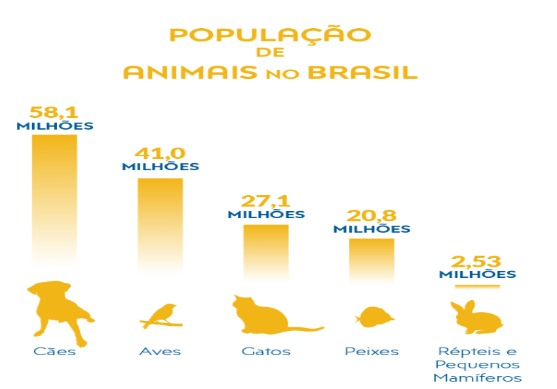
\includegraphics{exemplos/diagramas/População_Animais.jpeg}
    \caption{A população de animais no Brasil no ano de 2021.}
    \label{fig:População_Animais}
    \fonte{Instituto Pet Brasil apud IBGE}
\end{figure}
\\
Considerando o grande número de pessoas com Pets(LINK AQUI) e o carinho que possuem por eles, criou-se   um certo medo de como seus animais serão tratados. Segundo o (Graf , 2016)(LINK AQUI) os donos de animais de estimação, no momento de escolher profissionais para cuidar de seus Pets(LINK AQUI), possuem muitos receios, no que tange a qualidade do serviço e o cuidado do profissional, além disso, o preço do serviço (Gráfico 2)(LINK AQUI).
Um método muito efetivo de conhecer a qualidade de um serviço é por indicação que uma pessoa recebe de um amigo ou conhecido,  nesse âmbito, a aplicação busca disponibilizar avaliações dos parceiros feitas por outros usuários. 
\begin{figure}
    \centering
    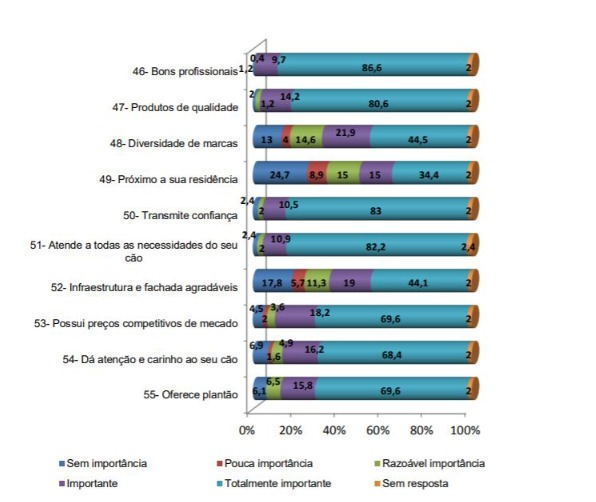
\includegraphics{exemplos/diagramas/graf_analise.jpeg}
    \caption{Principais motivos de escolha de Pet Shops. Os números indicam o número das perguntas, no questionário original da referência Graf (2016)(LINK AQUI)}
    \label{fig:graf_analise}
    \fonte{Graf (2016)(LINK AQUI)}
\end{figure}
\\

\subsection{Análise de concorrência}
Uma das ferramentas importantes no design de projetos é analisar empreendimentos similares e verificar os pontos positivos e negativos para justificar a criação de uma nova proposta. Entre os concorrentes atuais temos:
\begin{itemize}
    \item \textbf{PetDrive:}
        \begin{enumerate}
            \item \textbf{Pontos positivos:}
            Um dos aplicativos mais conhecidos pelo transporte de animais de estimação com seus donos, tendo como um de seus diferenciais o agendamento e equipamentos de transporte de animais dentro do carro disponibilizado pela empresa.
            \item \textbf{Pontos negativos:}
            Não disponibiliza a opção do cliente usar o seu próprio equipamento e não há a opção de viagens de animais desacompanhados.
    \end{enumerate}
    \item \textbf{Uber Pets}:
    \begin{enumerate}
            \item \textbf{Pontos positivos:}
            Conhecido dentro e fora do Brasil, interface intuitiva.
            \item \textbf{Pontos negativos:}
            Os carros não são adaptados para transporte de animais, não transportam o pet sozinho.
    \end{enumerate}
    \item \textbf{Mr. taxidog:}
    \begin{enumerate}
            \item \textbf{Pontos positivos:}
            Empresa antiga  no mercado, com profissionais qualificados e preparados no transporte de cachorros.
            \item \textbf{Pontos negativos:}
            Não é possível transportar outros pets como gatos e pássaros. Funciona somente no estado do Paraná.
    \end{enumerate}
    \item \textbf{Driver dog:}
    \begin{enumerate}
            \item \textbf{Pontos positivos:}
            Empresa com mais de 14 anos no mercado. Possui profissionais qualificados para lidar com cães, e transporte por longas distâncias.
            \item \textbf{Pontos negativos:}
            Não é possível transportar outros seres como gatos, coelhos,etc.
    \end{enumerate}
    \item \textbf{Dog hero:}
    \begin{enumerate}
            \item \textbf{Pontos positivos:}
            Possui profissionais qualificados na área de saúde animal, hospedagem de pets e creche. Está disponível em todo o Brasil.
            \item \textbf{Pontos negativos:}
            Aplicativo pouco intuitivo de transporte com veículo.
    \end{enumerate}
\end{itemize}

Analisando todos os concorrentes vemos que existe espaço para competitividade e crescimento de um novo produto. Portanto, o Carrara Pets busca trazer uma nova experiência para seus clientes , trazendo inovação, facilidade e mais funcionalidades para o cliente e seu pet, não se propondo a só transportar e cuidar dos pets, mas também buscar parcerias que agreguem mais valor para o negócio e satisfação ao consumidor final.

\begin{quadro}[thb]
\centering
\ABNTEXfontereduzida
\caption{Comparativo entre concorrentes}
\label{quadro-poluido-limpo-desalinhado}
\begin{tabular}{|l|l|l|l|l|l|l|}
\hline
\thead{Recursos} & \thead{Pet\\Driver} & \thead{Uber\\Pets} & \thead{Carrara\\Pets} & \thead{Mr.\\Taxidog} & \thead{Driver\\Dog} & \thead{Dog\\Hero}  \\
\hline
Transportar animais & \circlemark & \circlemark & \circlemark & \circlemark & \circlemark & \\
\hline
Corridas agendadas &\circlemark& &\circlemark& & &\circlemark\\
\hline
Serviços prestados pelo motorista & & &\circlemark& & &\\
\hline
Acompanhamento de viagem  &\circlemark&\circlemark&\circlemark& & &\circlemark\\
\hline
Hospedagem & & &\circlemark& & &\circlemark\\
\hline
Creche & & &\circlemark& & &\circlemark\\
\hline
Viagem compartilhada & & & &\circlemark& & \\
\hline
\end{tabular}
\fonte{Os autores.}
\end{quadro}

\section{Estrutura do Documento}
O presente documento está estruturado em 5 capítulos. O Capítulo 1(LINK AQUI), traz a contextualização do tema do projeto e a solução proposta, além de mostrar o objetivo geral e o objetivo específico, que deseja-se conquistar no desenvolvimento da aplicação. Ademais, possui a justificativa para a solução e uma análise de concorrência, demonstrando quais seriam os recursos disponíveis na plataforma Carrara Pets. Para finalizar, o capítulo contém esta seção para explicar a estrutura do documento. \\
No Capítulo 2(LINK AQUI), Revisão da Literatura, reúne-se as referências que forneceram embasamento para o trabalho. Neste capítulo, o leitor contará com temas referentes à aplicativo e público alvo, pontos principais da aplicação.\\
O Capítulo 3(LINK AQUI), Gerenciamento do Projeto, possui seções direcionadas a organização da equipe, falando sobre a metodologia que está sendo utilizada, links que contém algumas informações, como o canal do YouTube, blog da equipe e entre outros. \\
O Capítulo 4(LINK AQUI), Desenvolvimento do Projeto, aborda sobre as tecnologias utilizadas, viabilidade da aplicação, mostra os itens do escopo do projeto, apresenta a arquitetura da aplicação, a modelagem de dados e o diagrama de classes; explica sobre os padrões de projeto, sobre a segurança da informação e outros tópicos referentes ao desenvolvimento da aplicação.\\
Por fim, o Capítulo 5(LINK AQUI) é composto pelo resumo do projeto, explicitando as dificuldades de implementar o Carrara Pets e os obstáculos que apareceram durante o desenvolvimento e as funcionalidades futuras que poderão ser adicionadas à aplicação.\\
Além destes capítulos, o documento contém uma seção de Apêndice, com os documentos extras criados pela equipe ao decorrer do desenvolvimento, que acrescentam informações e melhoram o entendimento do projeto.


\newpage
\section{Processos}
\begin{itemize}
    \item Acompanhamento do veículo 
    \item Diagnóstico do atendimento (Veterinário)
    \item Possível cobrança em casos de compra de remédio
    \item Definição de rota para viagem
    \item Método de fidelidade (Pontos)
    \item Salvar acontecimentos da corrida em forma do tempo
    \item Fidelidade de motorista “X” pet (rotina)
    \item Compatibilidade do porte do pet com dimensões do veículo
    \item Validação do cadastro do motorista (Nome, Idade, Carro, Placa, CNH, CPF, Pré-entrevista com psicólogo(a))
    \item Cadastro de características
    \item Cadastro do pet (Tamanho, Peso, Porte, Temperamento)
    \item Cadastro do dono (Nome, CPF, Idade, Telefone, Endereço...)

\end{itemize}



% ---
% Capitulo de revisão de literatura
% ---
\chapter{Revisão da Literatura}

Na antiguidade, os seres humanos e outros animais caçavam devido a seu instinto, porém em algum momento, os seres humanos entenderão que ao domesticar esses animais poderiam ter maior efetividade no seu dia a dia. No decorrer do tempo, o ser humano descobriu que ao coexistir com animais, eles os tornavam mais fortes e felizes, foram inseridos cada vez mais em seu cotidiano até se tornarem parte da família, como seres de estimação, companheiro fiel e um apoio emocional (PESSANHA; PORTILHO, 2008)(LINK AQUI).
Olhando a sociedade moderna, onde esses animais se tornaram extremamente valorizados, de modo que chegam a substituir filhos. Muitas pessoas desistem de ter filhos para ter um animal tratado como tal (PESSANHA; PORTILHO, 2008)(LINK AQUI).

\section{Aplicativos}
Com o desenvolvimento da tecnologia o uso de aparelhos celulares e seus aplicativos têm se tornado essenciais no cotidiano das pessoas, por inúmeros motivos como facilidade para acessar contas bancárias, solicitar transporte, pedir uma refeição etc. Tudo isso de maneira rápida e extremamente acessível. Segundo pesquisas, o Brasil possui um grande potencial no âmbito de dispositivos móveis, cerca de 29\% da população utiliza aplicativos para atividades corriqueiras. Outra pesquisa mostra que as pessoas do Brasil ficam em torno de 3 horas em frente ao celular diariamente, superando países como EUA. (CARVALHO, 2003; GLOBOESPORTE.COM, 2019; SANTOS, 2020; BRITO, 2021)(LINK AQUI).\\
No projeto, a ideia de criar um aplicativo ao invés de um WebApp ou uma aplicação Web, deu-se o intuito de ter maior credibilidade e funcionalidade na aplicação, além de usar uma baixa quantidade de dados móveis para o cliente final.

\section{Público alvo}
Silva (2021) apud Graf (2016) Diz que os animais são atualmente tratados como membros da família. Segundo Silva et.al. (2021), a relação entre seres domesticados e seus donos pode ser separada em:
\begin{itemize}
    \item \underline{" Afeto: O dono usa mais serviços/produtos de alta qualidade, como enfeites, xampu\\, roupas etc.;" }
    \item \underline{"Interação: Onde o dono contrata serviços de adestramento para adequar o animal \\ao seu estilo de vida e produtos para o bem-estar dele;"}
    \item \underline{"Substituição humana: O consumidor substitui as relações humanas, como filhos ou \\amigos, pelo animal de estimação, pagando por atividades de tratamentos \\veterinários de luxo, adestramento e atividades geralmente associadas a relações humanas,\\ como funerais.”}
\end{itemize}

% ---

% ---

% ---

\chapter{Gerenciamento do Projeto}
Neste capítulo é apresentado o gerenciamento do projeto e todas as etapas seguidas, dentre estas destacam-se as reuniões e Sprint.
\\

\section{Metodologia}
A metodologia de gerenciamento do projeto utilizada é o Scrum, um Framework que tem como objetivo viabilizar o gerenciamento ágil de projetos de software, através de práticas e técnicas que garantem a comunicação efetiva dos integrantes, facilitando o aprendizado e a melhoria contínua das pessoas envolvidas no projeto. \\
Seguindo esse \textit{Framework(LINK AQUI)}, o projeto possui um conjunto de atividades que devem ser executadas em iterações semanais, as quais são chamadas de \textit{Sprint(LINK AQUI)}. De início, são criadas atividades e funcionalidades para o projeto, que são chamadas de \textit{Product Backlog}. Ao iniciar uma \textit{Sprint(LINK AQUI)}, é realizado uma reunião com a equipe para definir quais funcionalidades devem ser implementadas do \textit{Product Backlog}, essa reunião é conhecida como\textit{ Sprint Planning}, as tarefas selecionadas pela equipe são chamadas de \textit{Sprint Backlog} e as funcionalidades escolhidas são definidas como \textit{Users Stories}. Ao final da Sprint(LINK AQUI), a equipe apresenta as funcionalidades implementadas em outra reunião chamada \textit{Sprint Review}, e após isso, o ciclo se reinicia.
\\

\section{Organização da equipe}
A equipe é composta por 5 membros que foram definidos no primeiro dia de aula, onde houve a apresentação da disciplina. Com a equipe formada foi decidido o papel de cada pessoa dentro do projeto de acordo com a experiência de cada um. \\
O Quadro 2 apresenta o papel de cada pessoa no projeto. Vale ressaltar que os integrantes não farão atividades apenas voltadas ao que está no quadro, mas que darão um foco maior nas atividades descritas.
\begin{quadro}[thb]
\centering
\ABNTEXfontereduzida
\caption{Organização da equipe}
\label{quadro-poluido-limpo-desalinhado}
\begin{tabular}{|l|l|l|l|l|l|}
\hline
\thead{Atividades} & \thead{Davi} & \thead{Fabricio} & \thead{José} & \thead{Lorena} & \thead{Guilherme}\\
\hline
Arquitetura& & & \circlemark & & \circlemark \\
\hline
Banco de dados& & \circlemark & \circlemark & & \circlemark \\
\hline
Blog& \circlemark & & & \circlemark & \\
\hline
Código Latex& & \circlemark & & & \\
\hline
Desenvolvimento back-end& & \circlemark & \circlemark & & \circlemark \\
\hline
Desenvolvimento front-end& \circlemark & & & \circlemark & \\
\hline
Documentação& \circlemark & \circlemark & \circlemark & \circlemark & \circlemark \\
\hline
Gerência& & & & \circlemark & \\
\hline
Youtube& \circlemark & & & & \\
\hline
\end{tabular}
\caption{Organização da equipe}
\fonte{Os autores.}
\end{quadro}

O Davi é responsável por realizar as atualizações do blog(LINK AQUI) semanalmente e das apresentações no Youtube e também fará parte do desenvolvimento front-end do projeto.\\ 
O Fabrício é responsável pelo banco de dados e diagramas e é o líder na área de LATEX o trabalho dele será direcionar, ensinar e revisar os códigos LATEX da documentação. \\
O José está encarregado de cuidar do banco de dados juntamente com Fabrício além de ser responsável pelo design de arquitetura e preparar o ambiente de desenvolvimento na primeira etapa do projeto. No decorrer do desenvolvimento ele fará a programação back-end juntamente com o Fabrício.  \\
A Lorena é a gerente de projetos e tem como atividade liderar, organizar, estimular a equipe a sempre trabalharem juntos e compartilhar das dificuldades. Atua no desenvolvimento front-end e realiza as atualizações do blog juntamente com o Davi semanalmente. \\
O Guilherme é responsável pelo design da aplicação, paleta de cores, warframe e suporte na parte de back-end(LINK AQUI) do projeto.\\
Todos os integrantes são responsáveis pelo desenvolvimento da documentação e pela realização dos testes unitários.
\\

\section{Comunicação da equipe}
A equipe disponibiliza vários links com os recursos aqui produzidos, nesses links encontram-se informações sobre o trabalho, documentos, relatos semanais e vídeos de desenvolvimento do projeto(Reuniões e apresentações).  \\
	A \ref{QRYoutube} indica o link para o Youtube utilizado pela equipe para compartilhamento de reuniões, apresentações e etc.\\
Os links das \ref{QRTrello} é referente ao Trello, ferramenta de gerenciamento utilizado pela equipe no início do projeto, nesses sites é possível encontrar o planejamento do projeto.\\
A \ref{QRSVN} indica o link para o repositório Subversion utilizado pela equipe para compartilhamento de arquivos e entrega de documentos.\\
Como requisito da disciplina, o projeto deve ser relatado em um blog, disponível em \ref{QRBlog}.\\
Como objeto adicional para o projeto foi criado um wireframe das telas da aplicação contextualizando, disponível em \ref{QRWireframe}.\\

\newpage
\begin{figure}
    \centering
    
\includegraphics{exemplos/QRCode/QR blog.PNG}
    \caption{QR Code - Blog}
    \underline{https://carrarapets.blogspot.com/2022/04/reuniao-com-o-professor-na-terca.html?zx=8b6f737ec7e5c039}
    \label{QRBlog}
\end{figure}
    
\begin{figure}
    \centering
    
\includegraphics{exemplos/QRCode/QR SVN.PNG}
    \caption{QR Code - SVN}
    \underline{https://svn.spo.ifsp.edu.br/svn/a6pgp/S202201-PI-NOT/Grupo4/}
    \label{QRSVN}
\end{figure}

\begin{figure}
    \centering
    
\includegraphics{exemplos/QRCode/QR trello.PNG}
    \caption{QR Code - Trello}
    \underline{https://trello.com/invite/b/VwkOBdgD/8de44bebb8430adfd8af3871dabc7d4c/projeto-pi1}
    \label{QRTrello}
\end{figure}
    
\begin{figure}
    \centering
    
\includegraphics{exemplos/QRCode/QR wireframe.PNG}
    \caption{QR Code - Wireframe}
    \underline{https://whimsical.com/wireframe-tcc-Hi9cvRoYkUbDLEa8K2UHcK}
    \label{QRWireframe}
\end{figure}

\begin{figure}
    \centering
    
\includegraphics{exemplos/QRCode/QR youtube.PNG}
    \caption{QR Code - Youtube}
    \underline{https://www.youtube.com/channel/UCi0IphrbwIS3ToNnYDU0mJQ/featured}
    \label{QRYoutube}
\end{figure}

    
\chapter{Desenvolvimento do projeto}
Neste capítulo é apresentado itens relacionados ao desenvolvimento, descrevendo as tecnologias utilizadas, escopo do projeto, dividido entre Prova de Conceito (POC)(LINK AQUI), MVP(LINK AQUI) e entrega final, arquitetura da aplicação, diagramas de modelagem e entre outros. \\
\section{Técnologias utilizadas}
As tecnologias que serão utilizadas para o desenvolvimento do aplicativo tem como o principal objetivo é deixar a aplicação flexível e viável com diferentes plataformas.\\
As ferramentas escolhidas são:
\begin{itemize}
    \item \textbf{Vscode :}
    Como IDE será usado o Vscode por sua praticidade no desenvolvimento de aplicativos e programas, além de ser super compatível com Javascript e Typescript.
    \item \textbf{JavaScript/TypeScript :}
    Como linguagem complementar do React native, além de usar o typescript para melhor estruturar o projeto no desenvolvimento.
    \item \textbf{React Native :}
    Será usado para desenvolver o aplicativo, visando atender sistemas Android e IOS de forma nativa, sendo totalmente compatível com Heroku.
    \item \textbf{Expo :}
    Consiste num conjunto de ferramentas voltadas para facilitar o desenvolvimento de aplicações mobile. Fornece diversos simplificadores para desenvolvimento e testes, sendo bem simples e prático no desenvolvimento da aplicação.
    \item \textbf{Express :}
    Como framework será utilizado o express tendo em conta que será usado Node.js na aplicação desenvolvida do projeto, e  por ser um framework minimalista e flexível.
    \item \textbf{PostgreSQL :}
    Por ser um banco de dados bem completo oferecendo a possibilidade de armazenar dados não relacionais, ele também é de fácil hospedagem no Heroku, disponibilizando a plataforma para uso gratuito em desenvolvimento.
    \item \textbf{Heroku :}
    Para a hospedagem é usado a Platform as a Service (PaaS)(LINK AQUI) Heroku, que oferece gratuitamente hospedagem que oferece para contas free 550 horas mensais de atividade de ‘app type’ (métrica de processamento da plataforma).
    \item \textbf{SVN :}
    Como uma das  ferramentas de versionamento, para gerenciar a documentação do projeto, geração de vídeos como os commits e modificações  realizadas pelos integrantes do grupo.
    \item \textbf{Docker :}
    Visando ter uma ferramenta de gerenciamento da infraestrutura aplicada será utilizado o Docker, criando uma maior agilidade na manutenção e modificação da aplicação.
    \item \textbf{Google Maps API :}
    O uso da API(LINK AQUI) do \textit{Google maps}, que disponibiliza um meio de cálculo de rotas, rastreio para acompanhar rotas, para deixar a aplicação mais completa.
\end{itemize}
    O aplicativo precisa fornecer recursos de integração com outras aplicações, isto é, autenticação utilizando API(LINK AQUI) do Google, facilitando o acesso e a criação de cadastros dos usuários.

\section{Viabilidade financeira de mantimento da aplicação}
A aplicação estará alocada no serviço de hospedagem do Heroku(LINK AQUI), que em seu plano gratuito, armazenará aplicativos não comerciais, MVPs e projetos pessoais (HEROKU, 2020)(LINK AQUI). Porém, a hospedagem é limitada, e por isso, considerando que a aplicação terá fins comerciais e futuramente será necessário aumentar a demanda de usuários, de modo que a equipe migraram para o serviço Heroku(LINK AQUI) padrão, que custa por volta de cinquenta dólares (US\$ 50) correspondente a duzentos e trinta e cinco reais e doze centavos (R\$ 235,12) mensais (HEROKU, 2020)(LINK AQUI).\\
Visando o melhor banco de dados foi identificado que o PostgreSQL(LINK AQUI) é o melhor primeiramente por ser gratuito, totalmente compatível com o Heroku(LINK AQUI), porém tendo a possibilidade de fazer doações a melhoria contínua do banco. Após o término do projeto será migrado para o plano standard com o custo de cinquenta dólares (US\$50) correspondente a duzentos e trinta e cinco reais e doze centavos (R\$235,12) mensais (HEROKU, 2020)(LINK AQUI).\\
O app será disponibilizado na Play Store(LINK AQUI) possuindo um custo fixo pago somente uma vez no valor de vinte e cinco dólares (US\$25), correspondente a cento e dezessete e cinquenta e cinco centavos  (R\$117,55 cotação atual) aproximadamente (GOOGLE PLAY CONSOLE,2022)(LINK AQUI).\\
O app também será disponibilizado na Apple Store(LINK AQUI) possuindo um custo fixo pago somente uma vez no valor de noventa e nove dólares (US\$99), correspondente a quatrocentos e sessenta e cinco reais e cinquenta e um centavos (R\$465,51 cotação atual) aproximadamente (APPLE DEVELOPER PROGRAM,2022)(LINK AQUI).\\
Para ter um maior controle da infraestrutura do projeto, agilidade de criação, manutenção e modificações de serviços o Docker(LINK AQUI) é a melhor escolha no plano gratuito, pensando em levar a aplicação adiante após a finalização do projeto, alterar o plano para o pro no valor de cinco dólares (US\$5) correspondente a vinte e tres reais e cinquenta e um centavos (R\$23,51 cotação atual) aproximadamente mensal (DOCKER,2022)(LINK AQUI)\\
Para o gerenciamento de Log, será utilizado o Papertrail(LINK AQUI), que é um software adicional no Heroku, disponibilizado no plano gratuito de dez megabytes por sete dias, porém pensando e no seguimento da aplicação, após o término do projeto, será alterado para o Plano Fixo por oito dólares (US\$8) correspondente a trinta e sete reais e vinte centavos (R\$37,20 cotação atual) aproximadamente mensal.\\
Com relação aos custos, a seguir há dois quadros que informam o custo da aplicação. O primeiro quadro (Quadro 3)(LINK AQUI) , mostra os custos durante o desenvolvimento da aplicação, também foi colocado o valor da licença da Play Store(LINK AQUI) e Apple Store(LINK AQUI) somente para ilustrar, por ser somente para o projeto a aplicação não será disponibilizada no momento.\\
O segundo quadro (Quadro 4)(LINK AQUI), informa o custo da aplicação mensal após o término do projeto, onde o grupo dá seguimento no projeto com fins lucrativos.

\newpage
\begin{figure}
    \centering
    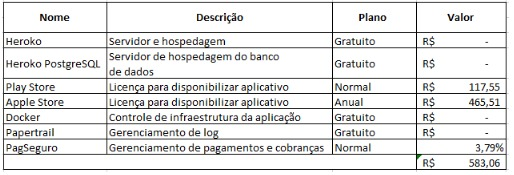
\includegraphics{exemplos/diagramas/Custo com despesas da aplicação no desenvolvimento.jpeg}
    \caption{Custo com despesas da aplicação no desenvolvimento}
    \label{fig:Custo com despesas da aplicação no desenvolvimento}
    \fonte{Os autores.}
\end{figure}\\

\begin{figure}
    \centering
    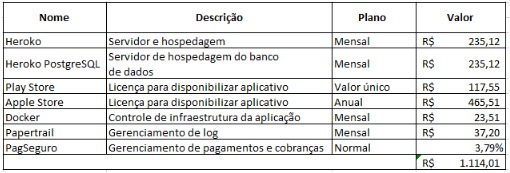
\includegraphics{exemplos/diagramas/Custo com despesas da aplicação após o término do projeto.jpeg}
    \caption{Custo com despesas da aplicação após o término do projeto}
    \label{fig:Custo com despesas da aplicação após o término do projeto}
    \fonte{Os autores.}
\end{figure}

\subsection{Captação de Receita}
Para a obtenção de fundos para a empresa e para o aplicativo, começaremos buscando parcerias, para incluir na aplicação, por esse meio, podemos fechar uma porcentagem, por indicação que pode variar de 5\% a 15\% do valor, inicialmente será variado, mas ao decorrer do tempo iremos ajustar os valores conforme o crescimento da empresa.\\
Com o tempo, prestaremos um serviço onde o parceiro poderá solicitar uma viagem em nosso aplicativo para buscar ou levar o seu animal em locais específicos, criando assim, uma parceria significativa, pois utilizaremos esse meio para ajudar a empresa terceira crescer, como também divulgaremos o nosso aplicativo para que outras empresas possam nos contratar para realizar esse tipo serviço. \\
Além das parcerias, iremos usar a opção de serviço de passeio do aplicativo para obter receita, na qual cobraremos o valor fixo de cinquenta reais (R\$50,00) a cada passeio solicitado pelo cliente. Também terá um serviço de compras dentro do aplicativo, onde forneceremos a opção do cliente disponibilizar o próprio alimento do animal ao motorista ou terá um campo específico para o cliente adicionar a compra da refeição do animal dentro do aplicativo e no final da corrida, será enviado um comprovante com os valores prestados pelo motorista. \\
E por último terá um método de viagem padrão, na qual teremos uma tarifa base de acordo com cada região, como o valor mínimo a receber, valor por minuto de viagem, valor por quilômetro rodado e o valor de serviço (do aplicativo) de 25\% que será cobrado em cada viagem ou serviço. \\
No Quadro 5(LINK AQUI) está demonstrando a cobrança da viagem padrão do passageiro e do motorista.\\

\newpage
\begin{figure}
    \centering
    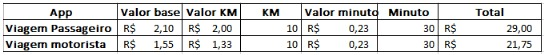
\includegraphics{exemplos/diagramas/Cálculo de viagem padrão.jpeg}
    \caption{Cálculo de viagem padrão}
    \label{fig:Cálculo de viagem padrão}
    \fonte{Os autores.}
\end{figure}\\
Para exemplificar a cobrança no quadro acima (Quadro 5)(LINK AQUI) foi realizado a fórmula: 
\mathrm{\textit{ Valor base + (Valor KM * KM) + (Valor minuto * minuto) = > Valor mínimo}}
\begin{itemize}
    \item Valor Base: é o valor fixo para se calcular a viagem;
    \item Valor KM: valor que será usado para calcular a quilometragem;
    \item KM: quilômetros percorrido na viagem;
    \item Valor Minuto: valor que será usado para calcular o minuto;
    \item Minuto: tempo de viagem em minutos;
    \item Valor Mínimo: é o valor que o motorista recebe de acordo com a região.
\end{itemize}
O cálculo acima mostrará como arrecadaremos fundos com a aplicação. \\
O Quadro 6(LINK AQUI) apresentado abaixo é o cálculo dos valores arrecadados em um dia versus a quantidade dos valores arrecadados pelo motorista em 10 horas de trabalho. \\
\newpage
\begin{figure}
    \centering
    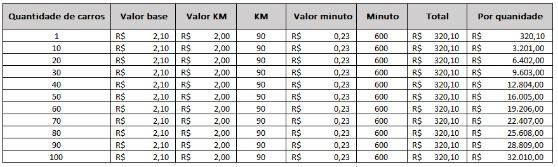
\includegraphics{exemplos/diagramas/Valor arrecadado em um dia versus quantidade de horas trabalhadas.jpeg}
    \caption{Valor arrecadado em um dia \textit{versus} quantidade de horas trabalhadas.}
    \label{fig:Valor arrecadado em um dia versus quantidade de horas trabalhadas.}
    \fonte{Os autores.}
\end{figure}\\
O Quadro 7(LINK AQUI) mostra o comparativo entre a receita mensal menos ( - ) o valor do custo mensal informado no Quadro 4(LINK AQUI).\\

\newpage
\begin{figure}
    \centering
    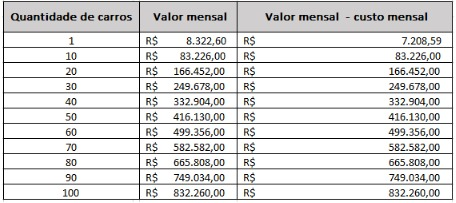
\includegraphics{exemplos/diagramas/Valor arrecadado mensal menos custo mensal.jpeg}
    \caption{Valor arrecadado mensal menos custo mensal.}
    \label{fig:Valor arrecadado mensal menos custo mensal.}
    \fonte{Os autores.}
\end{figure}\\

\section{Escopo do Projeto}
O escopo do projeto é definido para que a equipe consiga guiar as sprints e desenvolver a aplicação de maneira linear. Os itens descritos abaixo serão explicados mais adiante, na seção de requisitos funcionais, Apêndice E(LINK AQUI), requisitos não funcionais, Apêndice F(LINK AQUI) e histórias de usuários Apêndice D(LINK AQUI).

\subsection{Prova de Conceito}
A prova de conceito é utilizada para denominar um modelo prático que possa provar o conceito estabelecido neste projeto. Para a realização da POC, foi realizado o desenvolvimento do cadastro do usuário, pet e motorista e sua autenticação no sistema ao logar no Carrara Pets. 
\susection{Produto mínimo víavel (MVP)}
O MPV(LINK AQUI) define as funcionalidades essenciais para que o projeto funcione de maneira mais simples. Para isso, considera-se os itens desenvolvidos no POC(LINK AQUI) e mais alguns itens listados a seguir:
        \begin{itemize}
            \item Recuperar senha.
            \item Alterar dados cadastrados.
            \item Solicitação de transporte.
            \item Calcular tempo de viagem.
            \item Acompanhar viagem.
            \item Verificar forma de pagamento escolhida.
            \item Comparar saldo em conta com o valor da viagem.
            \item Cobrança de empresa externa para cartão.
            \item Finalizar viagem.
            \item Cancelar viagem.
            \item Avaliar viagem.
        \end{itemize}\\

\susection{Entrega Final}
Após entregar o POC(LINK AQUI) e MVP(LINK AQUI), buscamos finalizar a aplicação, seguindo o cronograma de planejamento criado no início do desenvolvimento desse projeto. Para a finalização da aplicação será necessário a inclusão de mais algumas funcionalidades, melhoria de algumas partes do desenvolvimento até o momento.
\begin{itemize}
    \item Comparar saldo em conta com o valor da viagem;
    \item Visualizar avaliações de outros usuários;
    \item Histórico de viagens;
    \item Indicação de parceiros;
    \item Catálogo de melhores motoristas por região;
    \item Personalização de fotos;
    \item Incluir valor adicional para o motorista;
    \item Criar tela de motoristas favoritos;
    \item Agendar viagens e serviços;
    \item Cobrança via cartão de crédito;
    \item Programa de pontos;
\end{itemize}\\
\section{Arquitetura da Aplicação}
Para a arquitetura do projeto foi definido a arquitetura em 3 camadas para melhor interação e controle. Por ser um método que proporciona 3 ambientes ou sistemas distintos, tornando assim o desenvolvimento mais ágil, escalabilidade mais simples e precisa, e menor possibilidade de indisponibilidade da aplicação e alto nível de segurança dos dados.\\
A arquitetura de três camadas é uma arquitetura de aplicativo de software bem estabelecida que organiza aplicativos em três camadas de computação lógica e física: a camada de apresentação ou interface do usuário; a camada do aplicativo, onde os dados são processados; e a camada de dados, em que os dados associados ao aplicativo são armazenados e gerenciados. (IBM, 2020)(LINK AQUI). Usando essa arquitetura teremos um método mais prático para escalar a aplicação, como também para trabalhar em partes específicas de modo que não prejudique a aplicação e a experiência do usuário.\\
\newpage
\begin{figure}
    \centering
    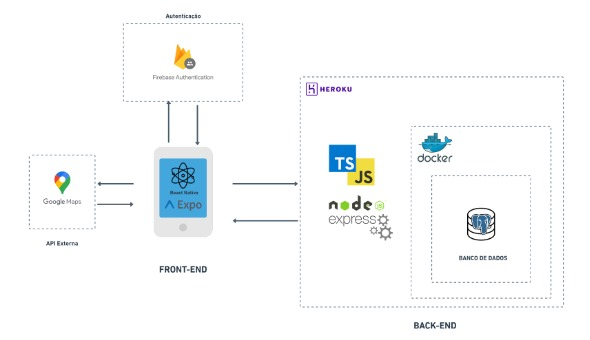
\includegraphics{exemplos/diagramas/Arquitetura Geral da Aplicação.jpeg}
    \caption{Arquitetura Geral da Aplicação}
    \label{fig:Arquitetura Geral da Aplicação}
    \fonte{Os autores.}
\end{figure}\\
Conforme o desenho da arquitetura geral, na parte do \textit{front-end(LINK AQUI)} da aplicação, teremos um sistema que rodará o \textit{Expo(LINK AQUI)} e \textit{React Native(LINK AQUI)}, desse modo, quando o cliente acessar o aplicativo abrirá a tela inicial e dará a opção de logar com a conta \textit{Google(LINK AQUI)} ou logar com a conta padrão. \\
Quando o cliente solicitar o acesso via Google, a aplicação irá acessar o \textit{Firebase(LINK AQUI)}, onde buscará junto ao \textit{Google API(LINK AQUI)} a validação da conta do cliente, e com isso, gerará um Token de validação que, devolverá o dado para o aplicativo, e por fim,  será enviado para o banco informando que o usuário estará se logando no aplicativo e salvando a informação. Diferente de quando o usuário decidir acessar com o endereço eletrônico e senha, o aplicativo levará os dados para o banco, validando a informação, e depois liberará  o acesso à conta do usuário.\\
Com o usuário dentro da aplicação, todos os dados processados do usuário serão enviados para o \textit{Docker(LINK AQUI)} avaliar, e depois será armazenado os dados no banco dentro do perfil do usuário.  \\
Como no início, a demanda será pequena, a equipe acompanhará esse processo para análise e melhoria, para diminuir o máximo possível a resposta e usabilidade da aplicação.\\

\subsection{Escalabilidade}
Escalabilidade de uma aplicação é a capacidade em que um sistema ou componente pode ser modificado para atender um ou mais problemas (GREGOL, 2011)(LINK AQUI). Atualmente, a escalabilidade deve estar sempre entre as prioridades (ENDEAVOR, 2015)(LINK AQUI), ou seja, a escalabilidade é uma característica desejada na aplicação.\\
Como um projeto é um aplicativo de transporte e tem potencial de aumento expressivo na quantidade de usuários e solicitações de acordo com seu crescimento. Por isso, é preciso da escalabilidade horizontal (GREGOL, 2011)(LINK AQUI), pois será necessário distribuir o processamento em diversas máquinas para que a aplicação responda rapidamente às requisições. Para atender essas solicitações, foi escolhido o PostgreSQL que possui a capacidade de expandir com facilidade sem perder a qualidade, de modo que agregam valor ao sistema. O Heroku(LINK AQUI), que será utilizado para escalar o sistema, limita seus recursos e serviços nos planos gratuitos, ou seja, no momento que for preciso escalar o sistema, precisará assinar planos para que possa consumir mais recursos dessas plataformas. Por isso, o Carrara Pets(LINK AQUI) usará a receita para arcar com essas despesas.\\
A necessidade de escalar o sistema provém para que a aplicação funcione de forma fluida e atenda as expectativas e satisfação dos usuários.

\section{Banco de Dados}
A aplicação tem como fonte de dados o Banco de Dados Relacional que, baseado no modelo, fornece acesso a pontos de dados relacionados entre si, possibilitando uma maneira intuitiva e direta de representar dados em tabelas. Neste modelo, cada linha na tabela é um registro com uma chave exclusiva, e suas colunas possuem atributos dos dados e cada registro. (ORACLE, 2022)(LINK AQUI). 

\section{Critérios de Segurança, Privacidade e Legislação}
    O aplicativo precisa gerenciar os dados e as informações pessoais do usuário de modo seguro, com o nível de permissão adequado(GOOGLE, 2022), visando a busca por definir medidas de manuseio e proteção dos dados dos usuários de qualquer que seja a aplicação. Será usada também a Lei Nº 13.853, implantada em 8 de julho de 2019, também chamada de Lei Geral de Proteção de Dados Pessoais (LGPD) (BRASIL, 2018).
    Como qualquer empresa séria que se preza, entende-se que os dados dos usuários e sua segurança são de extrema importância, com isso em mente, foram escolhidas as seguintes medidas de segurança:
\begin{itemize}
    \item \textbf{Senha com complexidade :} 
    O usuário na hora do cadastro no aplicativo irá solicitar que crie uma senha forte usando o padrão de no mínimo 8 dígitos com letras, números e pelo menos um caracter especial. Visando diminuir as chances de alguém adivinhar a senha, além de adicionar um limite de tentativas.
    \item \textbf{Verificação de duas etapas :} 
    Para validar e verificar a identidade do cliente, depois de se cadastrar no app é enviado um e-mail de validação para o usuário e um sms para verificar o telefone informado.
    \item \textbf{Criptografia de senha :} 
    Para a aplicação ser mais segura, será implantada a criptografia nos dados sensíveis dos clientes, como senhas, documentos dos clientes e dados bancários por meio de criptografia Hash.
\end{itemize}

\section{Critérios de LOG}
    Log é um arquivo de texto, XML e etc, que é gerado pela aplicação para descrever o seu funcionamento. Esse arquivo permite identificar problemas que podem estar ocorrendo dentro do sistema.
    Cada linha do Log contém uma informação a respeito de alguma alteração no software, ajudando a identificar falhas em requisições, respostas ou problemas nas funcionalidades do sistema.
    Para parte de logs será usado o Papertrail que é um software adicional do Heroku que analisa mensagens de log para detectar possíveis erros no sistema e disponibiliza notificações instantâneas automatizadas. 

\section{Processo de integração contínua}
    É uma prática de desenvolvimento de software em que os membros de uma equipe integram seu trabalho com frequência, geralmente cada pessoa integra pelo menos diariamente - levando a várias integrações por dia. Cada integração é verificada por uma compilação automatizada (incluindo teste) para detectar erros de integração o mais rápido possível (MARTIN , 2001).
    Para a melhoria contínua da aplicação, será utilizado o método de versionamento com o intuito de melhorar a aplicação criando melhoria de funcionalidades, correções de bugs, além de implementar novas opções e parcerias.

\section{Ferramentas para Testes automatizados e Análise Estática}
\textbf{Jest :} 
Para testes usaremos o Jest como principal framework para testes unitários e de unidade. O motivo pelo qual o escolhemos é principalmente pela sua simplicidade e facilidade de utilização e implementação.
\textbf{Testing Library :}
Também para os testes e para conseguir implementar o Jest para o mobile temos o Testing Library. Com muitas funcionalidades para facilitar a implementação e uma conversa muito boa com o Jest, esta será a nossa solução para testes.  
% Para facilitar a manutenção é sempre melhore criar um arquivo por capitulo, para exemplo isso não é necessário 

%---------------------------------------------------------------------------------------
\chapter{Modelo Teórico e Pressupostos (ou Hipóteses) da Pesquisa}




%---------------------------------------------------------------------------------------
\chapter{Métodos de Pesquisa}
\explicacao{Para trabalho da Pós Graduação}


\section{Tipo de Pesquisa}


\section{Plano Amostral (se Pesquisa Quantitativa)}


\section{Instrumento de Pesquisa e Escalas Utilizadas (Escalas se Pesquisa Quantitativa)}


\section{Coleta de Dados}


\section{Análise de Dados}



%---------------------------------------------------------------------------------------
\chapter{Resultados da Pesquisa}
\explicacao{Para trabalho da Pós Graduação}

\section{Discussão dos Resultados Observados}


%---------------------------------------------------------------------------------------





\chapter{Modelagem de dados}

\begin{sidewaysfigure}[htb]
    \caption{MER}
    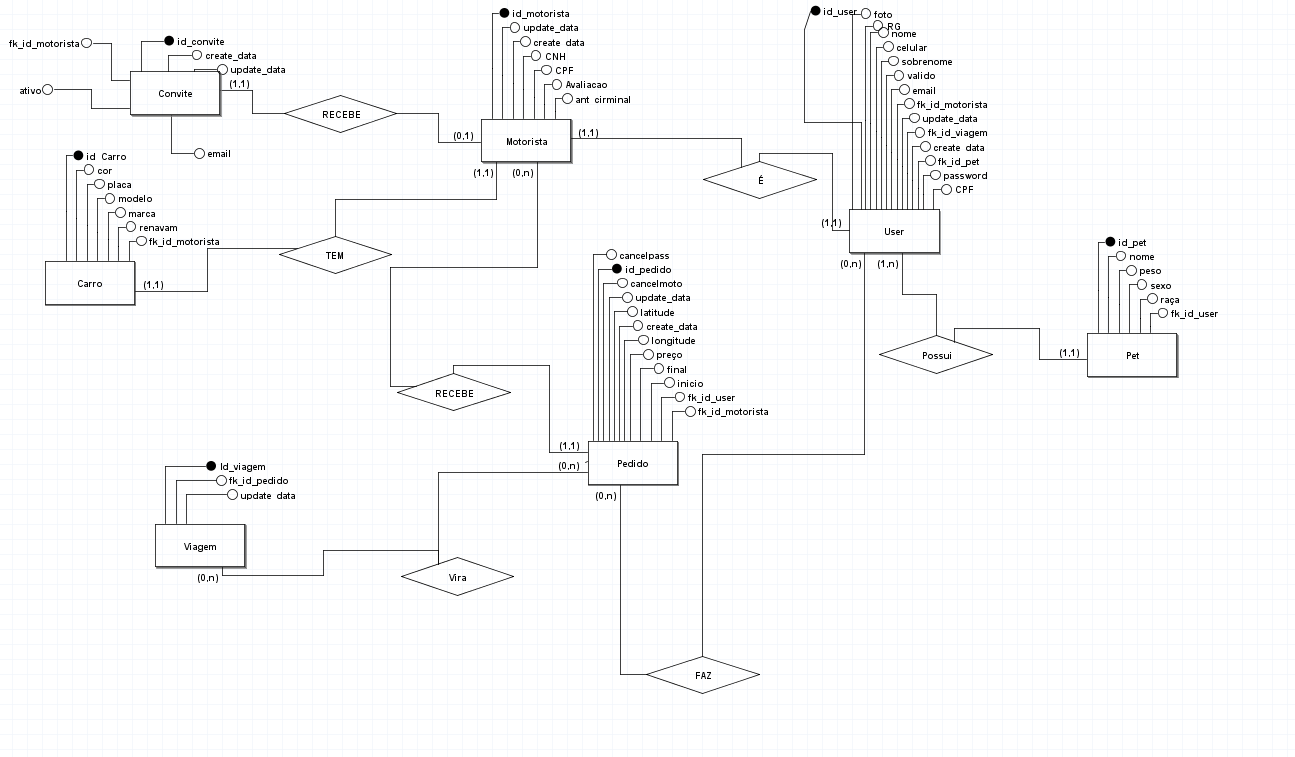
\includegraphics[width=0.9\textwidth]{exemplos/diagramas/mer.png}
    \fonte{Autores}
\end{sidewaysfigure}

\newpage
\begin{sidewaysfigure}[htb]
    \caption{DER}
    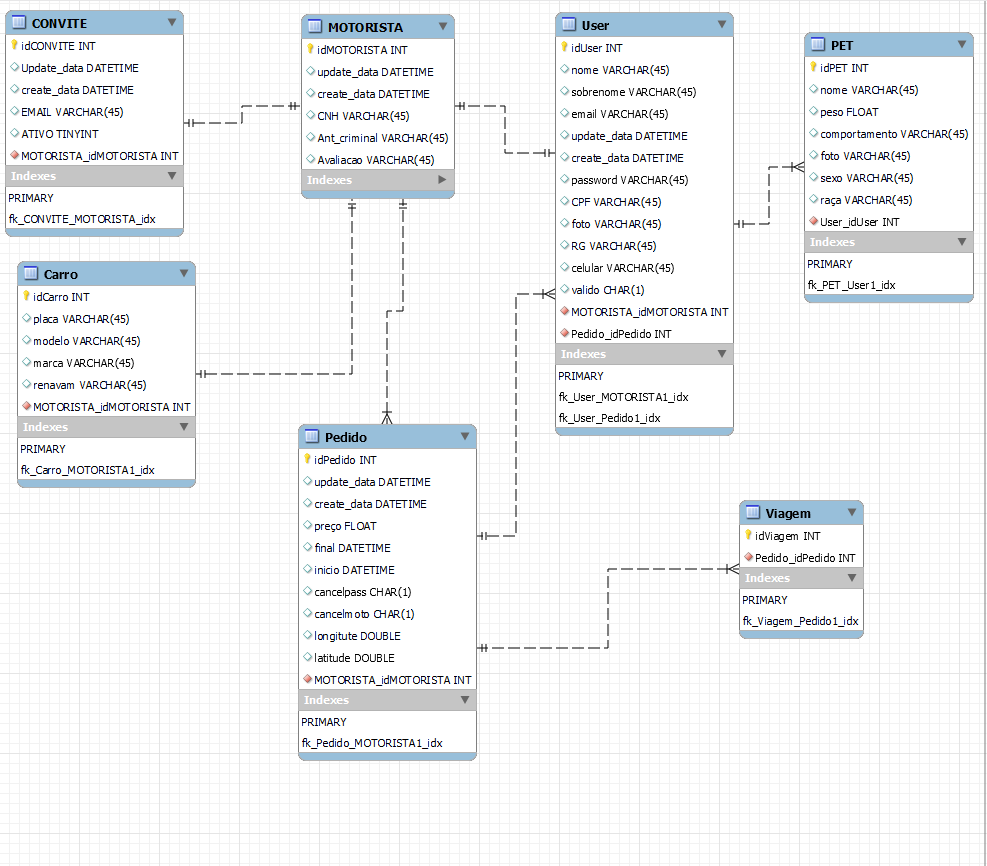
\includegraphics[width=0.7\textwidth]{exemplos/diagramas/der.png}
    \fonte{Autores}
\end{sidewaysfigure}

\newpage
%\begin{sidewaysfigure}[htb]
    \caption{Casos de uso - Cliente}
	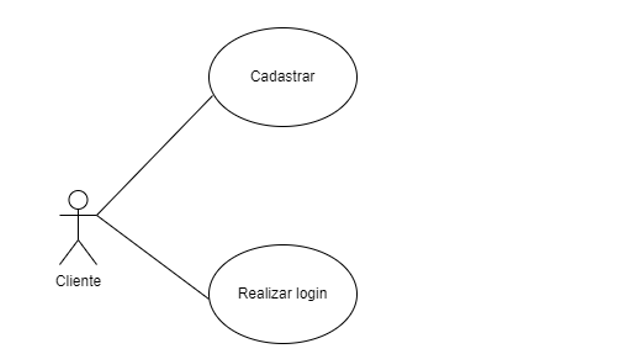
\includegraphics[width=0.9\textwidth]{exemplos/diagramas/Casos de uso_Cliente 1.PNG}
	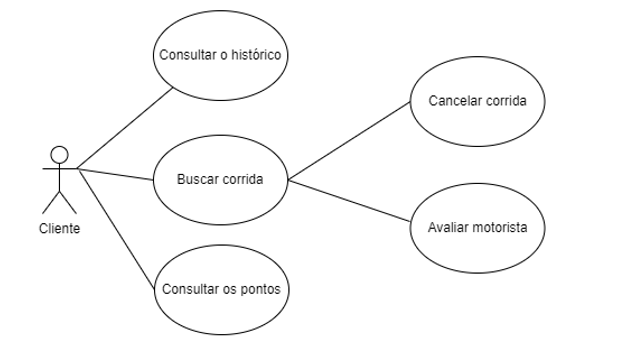
\includegraphics[width=0.9\textwidth]{exemplos/diagramas/Casos de uso_Cliente 2.PNG}
	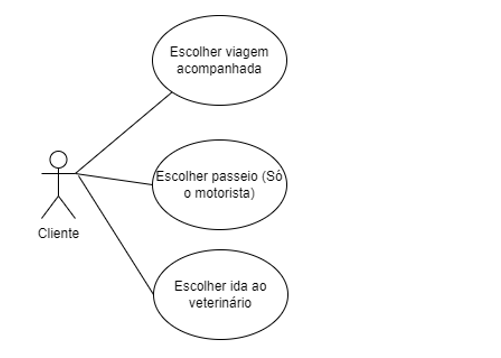
\includegraphics[width=0.9\textwidth]{exemplos/diagramas/Casos de uso_Cliente 3.PNG}
	\fonte{Autores}
%\end{sidewaysfigure}

\newpage
%\begin{sidewaysfigure}[htb]
    \caption{Casos de uso - Motorista}
	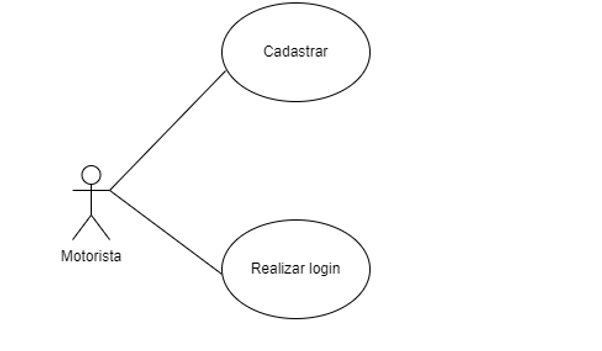
\includegraphics[width=0.8\textwidth]{exemplos/diagramas/Casos de uso_Motorista 1.PNG}
	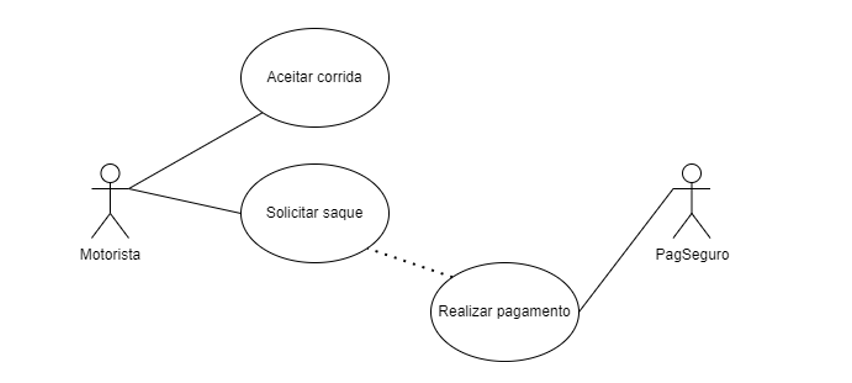
\includegraphics[width=0.8\textwidth]{exemplos/diagramas/Casos de uso_Motorista 2.PNG}
	\fonte{Autores}
%\end{sidewaysfigure}

\newpage
\begin{sidewaysfigure}[htb]
    \caption{Diagrama de classe}
    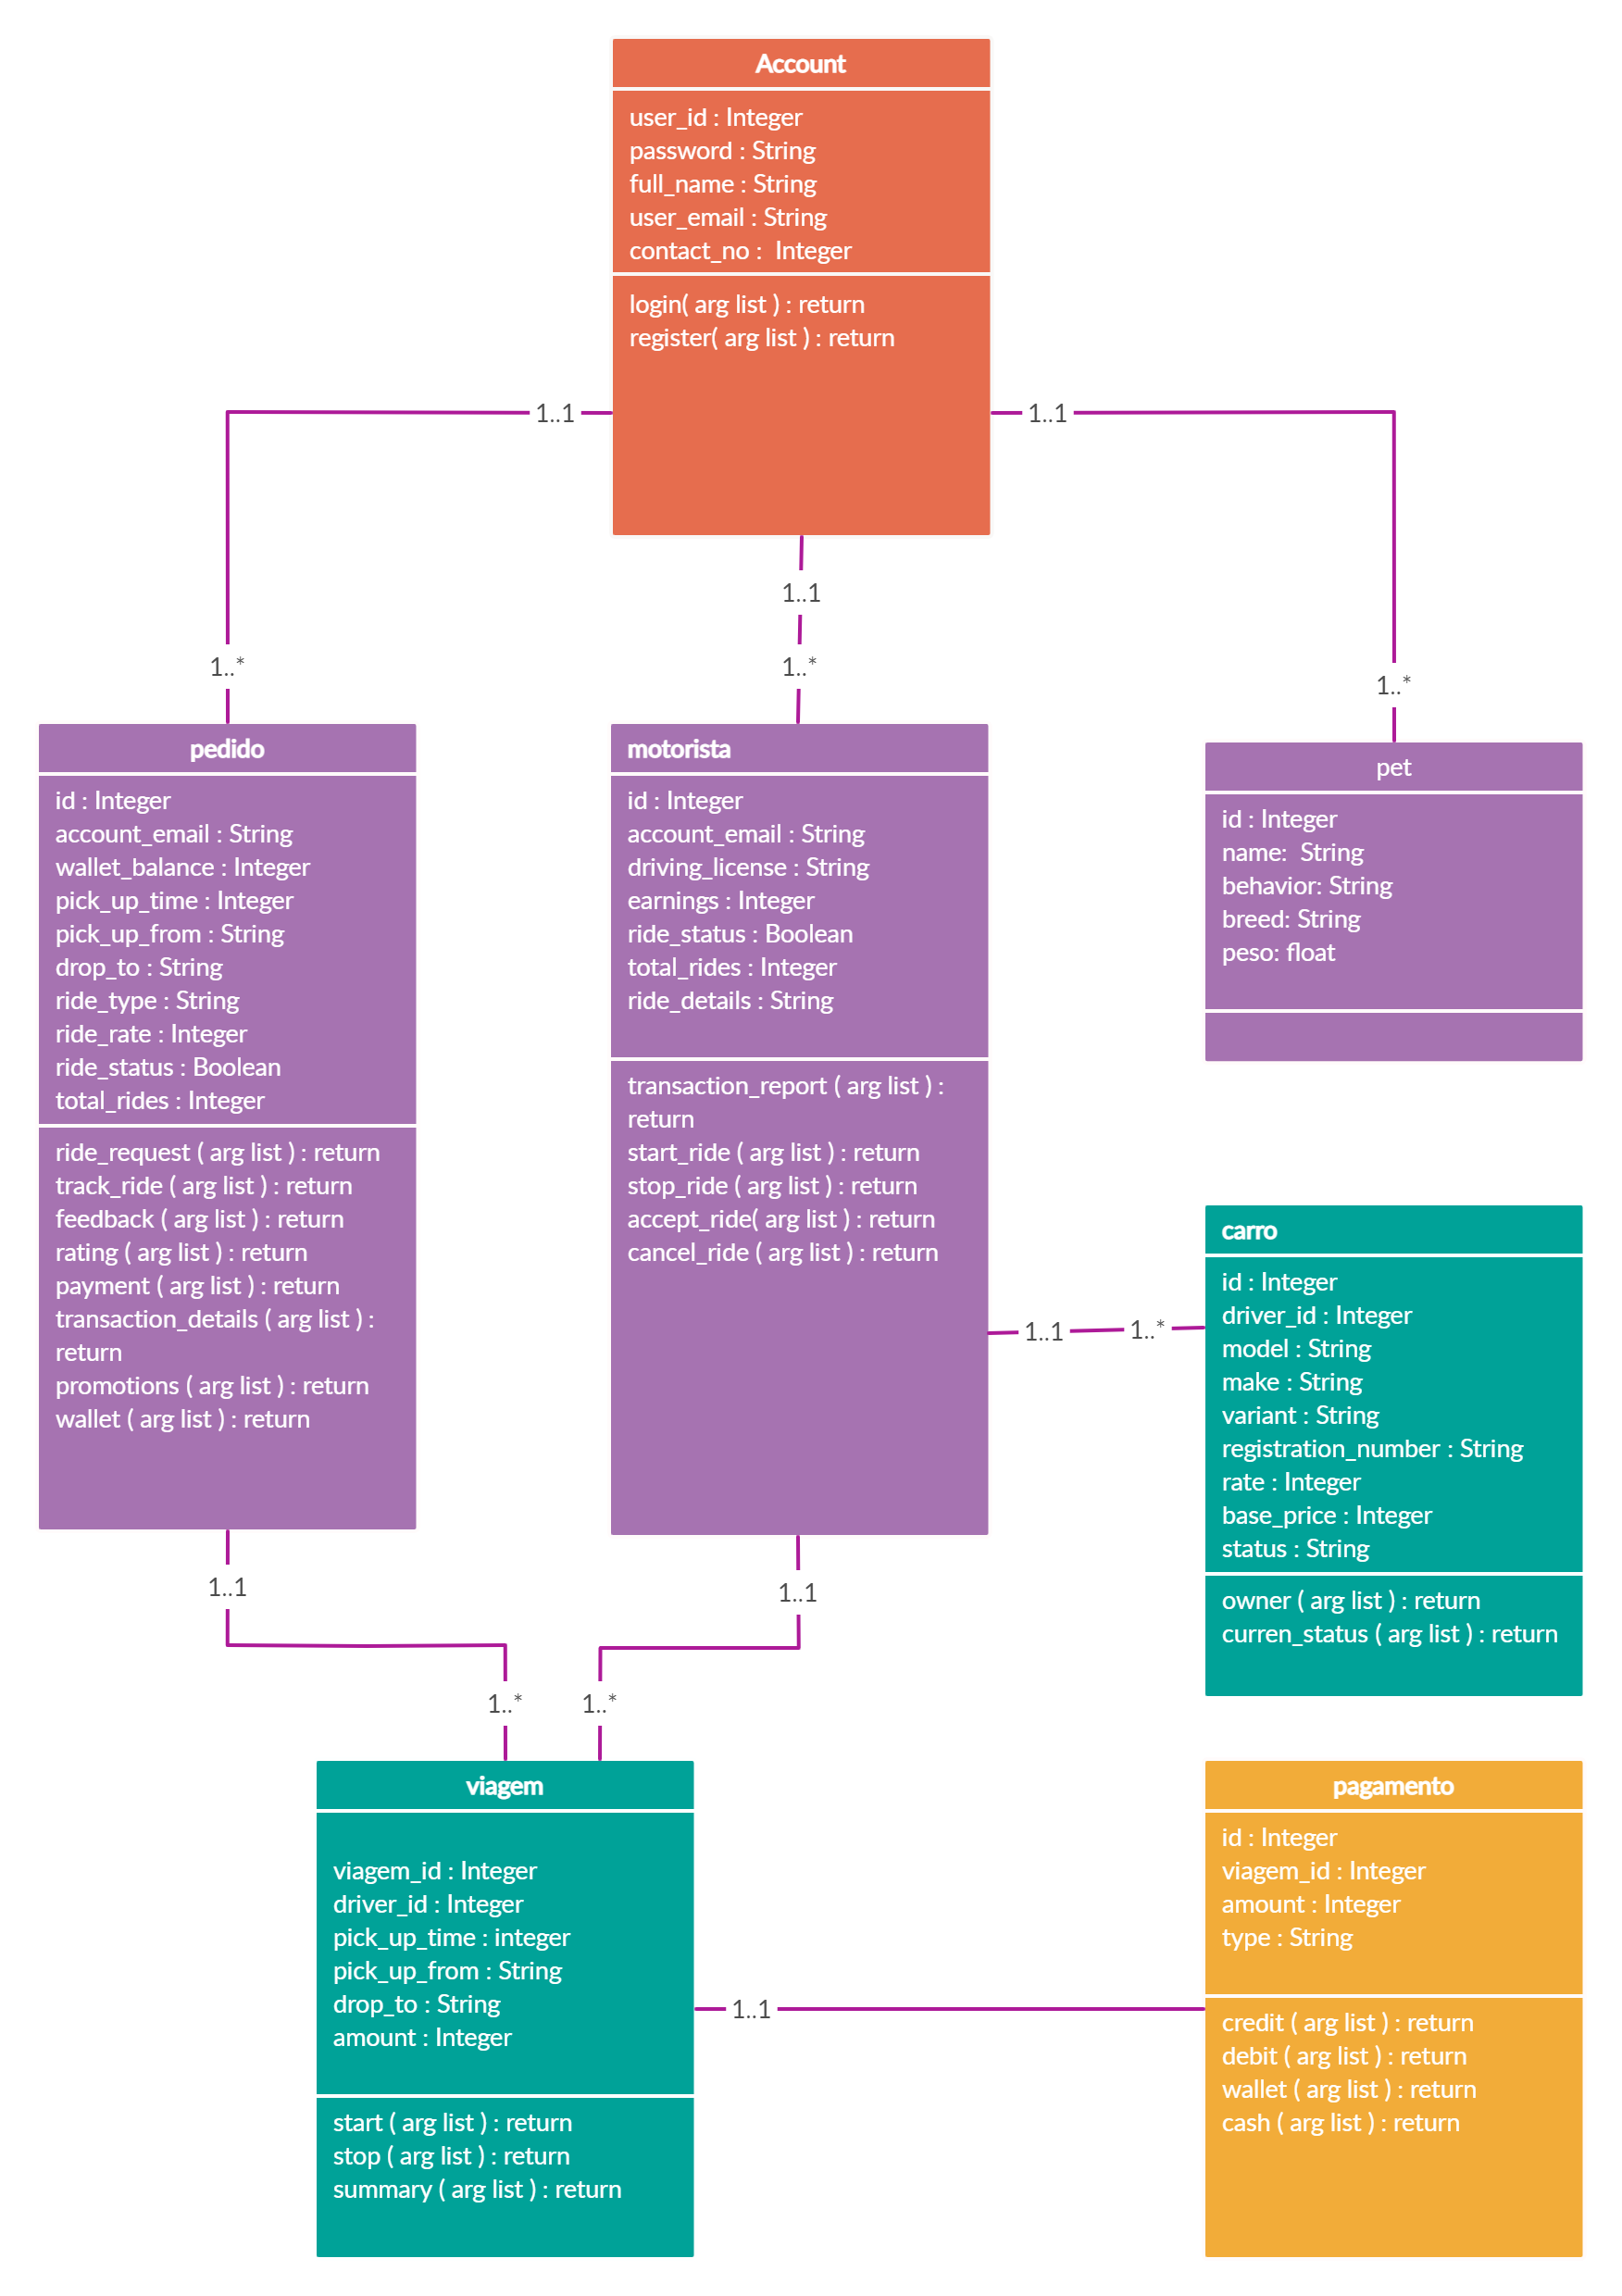
\includegraphics[width=0.5\textwidth]{exemplos/diagramas/tcc-diagram-class.png}
    \fonte{Autores}
\end{sidewaysfigure}



% Para facilitar a manutenção é sempre melhore criar um arquivo por capitulo, para exemplo isso não é necessário 



% exemplos de escrita LaTeX e erros comuns
%\chapter{Exemplos \LaTeX}
\label{cap-exemplos}

\explicacao{ATENÇÃO : Este capítulo e os seguintes demonstram como fazer no {\LaTeX} portanto devem ser lidos em conjunto com o código fonte desse documento}

% exemplo de como inserir uma referencia adicional no sumario (normalmente não utilizado em um trabalho acadêmico)
\addcontentsline{toc}{chapter}{Exemplos que devem ser lidos (mas esse tipo de indicação não vai em um trabalho acadêmico) :-)}

Esse capítulo tem exemplos de escrita utilizando o {\LaTeX}  utilizando \abnTeX, é muito simples escrever em \textbf{negrito}, \textit{itálico} \footnote{apesar de que nesse documento \mostraComandoLaTeX{textit} \mostraComandoLaTeX{emph} tem comportamento parecido é recomendável utilizar \mostraComandoLaTeX{textit} de forma genérica para itálico}, ....


Existem diversos tutoriais para uso de \LaTeX, se você está utilizando esse modelo não precisará se preocupar com muitos dos detalhes técnicos do \LaTeX \space e cuidar somente do seu texto.

Escolha seu editor : \url{https://en.wikipedia.org/wiki/Comparison\_of\_TeX\_editors}, apesar do overleaf sem bem prático, nem todas as funções estão disponíveis na versão gratuita e você pode instalar gratuitamente em seu computador um compilador \LaTeX \space e utilizar um sistema de controle de versão para gerenciar seu documento.


\section{Normas ABNT}

Esse documento modelo já resolve boa parte da padronização NBR 14.724:2011 \cite{NBR14724:2011} que deve ser seguida e inclusive alguns pontos que não são claros pelo modelo de padronização do \ac{ifsp}.

Leia os documentos do {\abnTeX} e do \ac{ifsp}:
\begin{itemize}
    \item \url{https://www.abntex.net.br/}
    
    \item \acs{faq} : \url{https://github.com/abntex/abntex2/wiki/FAQ}
    
    \item \url{http://mirror.unl.edu/ctan/macros/latex/contrib/abntex2/doc/abntex2.pdf}
    
    \item \waUrl{https://spo.ifsp.edu.br/biblioteca?id=184}
\end{itemize}

No \ac{ifsp} você pode acessar todas as normas \ac{abnt} sem custo, as informações estão disponíveis no endereço \waUrl{https://www.ifsp.edu.br/index.php/outras-noticias/52-reitoria/2329-alunos-e-servidores-do-ifsp-podem-acessar-abnt-via-web.html}.

Apesar de alguns elementos serem opcionais na \ac{abnt} eles foram definidos como obrigatórios (folha de rosto, resumo, lista de siglas, lista de ilustrações, glossário etc), nos trabalhos completos de projetos de informática do \ac{ifsp} campus São Paulo. Documentos menores como propostas de projeto, documento de \ac{poc} não necessitam desses elementos, mas alguns podem ser uteis para ajudar no estudo do {\LaTeX} em preparação para o documento final.

\begin{itemize}
    \item Logotipo da instituição, não é citado na \ac{abnt} nem no manual de normalização do \ac{ifsp}, mas aparece em uma imagem do documento de normalização, foi definido que não deve ser incluído na capa;
    
    \item Nome da instituição que é opcional na capa, deve ser utilizado;
    
\end{itemize}



\section{Detalhes textuais}

O documento é dividido em capítulos, e cada capítulo dividido em seções utilizando o \abnTeX \space você pode dividir seus documentos nos níveis de acordo com os comandos:

\begin{itemize}
    \item \mostraComandoLaTeX{chapter}  (1);
    
    \item \mostraComandoLaTeX{section} (1.1);
    
    \item \mostraComandoLaTeX{subsection} (1.1.1);
    
    \item \mostraComandoLaTeX{subsubsection} (1.1.1.1);
    
    \item \mostraComandoLaTeX{subsubsubsection} (1.1.1.1.1).
    
\end{itemize}

Tenha em mente que normalmente se utiliza no máximo o nível \mostraComandoLaTeX{subsection}.
Ao definir as divisões do seu trabalho utilizando as diretivas do \LaTeX, elas são automaticamente inseridas no sumário do documento.


\subsection{Caracteres Reservados e auxiliares}



Alguns caracteres são reservados no \LaTeX \space e por isso para utilizar esses caracteres é necessário utilizar uma forma diferenciada de escrita. É possível utilizar a macro \mostraComandoLaTeX{symbol} com o código \ac{ascii} do caracter desejado, veja no código fonte desse texto como utilizar corretamente esses itens.


\begin{itemize}
\item barra invertida : \textbackslash   \symbol{92}    $\backslash$;
\item til  :  \symbol{126} ;
\item cifrão : \$;
\item sublinhado, \textit{underscore}, \textit{underline} : \_;
\item \enquote{aspas} as macros \mostraComandoLaTeX{enquote} / \mostraComandoLaTeX{textquote} garantem o espaçamento correto, se utilizar diretamente as ASPAS o espaçamento é perdido;
% https://tex.stackexchange.com/questions/80395/no-space-after-closing-double-quote
\item marcadores : \cmark\ \xmark\ \circlemark\ \ding{100} \ - ver mais no \refanexo{pifont-quickref};
\item chaves : \} \{.
\end{itemize}

\subsection{Listas}

Em uma lista de itens cada item deve ser terminado por ponto e virgula, exceto o ultimo item que deve ter um ponto final.

\begin{itemize}
\item item 1;
\item item 2;
\item item ..;
\item item final.
\end{itemize}


\chapter{Referências}
ABINPET. Mercado Pet Brasil 2021. Disponível em: <http://www.abinpet.org.br/download/abinpet_folder_2021.pdf> Acesso em 14 de Abril de 2022.
INSTITUTO PET BRASIL.Censo Pet: 139,3 milhões de animais de estimação no Brasil.2019.Disponível em: <http://institutopetbrasil.com/imprensa/censo-pet-1393-milhoes-de-animais-de-estimacao-no-brasil/> Acesso em: 14 de Abril de 2022.
GOVERNO FEDERAL DO BRASIL. O Brasil registrou mais de 234 milhões de acessos móveis em 2020. Agência Nacional de Telecomunicações. 2021. Disponível em: <https://www.gov.br/pt-br/noticias/transito-e-transportes/2021/05/brasil-registrou-mais-de-234-milhoes-de-acessos-moveis-em-2020> Acesso em: 14 de Abril de 2022.
HEROKU. Heroku Pricing. 2020. Disponível em: <https://www.heroku.com/pricing#app-types-header>.Acesso em: 14 abr. 2022.
RIBEIRO, A. F. de A. Cães Domesticados e os benefícios da interação. Revista Brasileira de Direito Animal, Salvador, v. 6, n. 8, 2014. DOI: 10.9771/rbda.v6i8.11062. Disponível em: https://periodicos.ufba.br/index.php/RBDA/article/view/11062. Acesso em: 14 abr. 2022.
SILVA, N. A.; MARISCO, G. A RELAÇÃO DE ANIMAIS DOMÉSTICOS NA EDUCAÇÃO E SAÚDE. Interfaces Científicas - Saúde e Ambiente, [S. l.], v. 7, n. 1, p. 71–78, 2018. DOI: 10.17564/2316-3798.2018v7n1p71-78. Disponível em: https://periodicos.set.edu.br/saude/article/view/5491. Acesso em: 14 abr. 2022.
SOUZA, A. S. de. Direitos dos animais domésticos: análise comparativa dos estatutos de proteção. Revista de Direito Econômico e Socioambiental. v. 5, n. 1, p. 110–132, 2014. Disponível em: <https://periodicos.pucpr.br/direitoeconomico/article/view/6242>. Acesso em: 14 abr. 2022.
GOOGLE PLAY CONSOLE. Disponível em: <https://play.google.com/console/u/0/signup>.Acesso em: 16 abr. 2022.
APPLE DEVELOPER PROGRAM.Isenção da taxa de assinatura no Apple Developer Program
. Disponível em: <https://play.google.com/console/u/0/signup>.Acesso em: 16 abr. 2022.
Docker. Docker Pricing. 2022. Disponível em: <https://www.docker.com/pricing/>.Acesso em: 16 abr. 2022.
GREGOL, R. E. W. Recursos de escalabilidade e alta disponibilidade para aplicações web.Repositório de Outras Coleções Abertas, p. 17–18, 2011.
ENDEAVOR. Quão longe sua ideia pode ir? Descubra avaliando a escalabilidade dela. 2015. Disponível em: <https://endeavor.org.br/estrategia-e-gestao/escalabilidade/>.Acesso em: 17 abr. 2022.
GOOGLE DEVELOPERS. Disponível em: <https://developer.android.com/docs/quality-guidelines/core-app-quality?hl=pt-br#sc>.Acesso em: 18 abr. 2022.
BRASIL. Lei Geral de Proteção de Dados (2018). 2018. Disponível em: <http://web.archive.org/web/20200915225322/http://www.planalto.gov.br/ccivil_03/_ato2015-2018/2018/lei/L13709.htm>. Acesso em: 18 abr. 2022.
 MARTIN FOWLER.Continuous Integration. 2001.Disponível em: <https://martinfowler.com/articles/continuousIntegration.html>.Acesso em: 18 abr. 2022.
PESSANHA, L.; PORTILHO, F. Comportamentos e padrões de consumo familiar em torno dos “pets”. IV ENEC - Encontro Nacional de Estudos do Consumo, 2008.
GRAF, C. T. O comportamento do consumidor no mercado pet e a relação entre os cães e as pessoas. Universidade Regional do Noroeste do Estado do Rio Grande do Sul, 2016.
CHEN, A.; HUNG, K.; PENG, N. A cluster analysis examination of pet owners ’consumption values and behavior –segmenting owners strategically. Journal of Targeting, Measurement and Analysis for Marketing, v. 20, n. 2, p. 117–132, 2012.
Silvaet.al.Petshow.2021.Disponível em:<https://svn.spo.ifsp.edu.br/svn/a6pgp/S202001-PI/HYVE/Documentos/5-EntregaFina>.Acesso em: 01 mai. 2022.
PRODEST.O uso de aplicativos na sociedade.Disponível em:
<https://prodest.es.gov.br/o-uso-de-aplicativos-na-sociedade#:~:text=Os\%20aplicativos\%20fazem\%20cada\%20vez,op\%C3\%A7\%C3\%B5es\%20de\%20lazer\%20com\%20facilidade.> Acesso em: 03 mai. 2022.
CARVALHO, J. O. F. D. O papel da interação humano-computador na inclusão digital. Transformação, V. 15, n. spe, p. 75-89. Campinas, Dezembro, 2003 .Disponível em: <http://www.scielo.br/scielo.php?script=sci_arttext&pid=S0103-37862003000500004&lng=en&nrm=iso>. Acesso em: 03 mai. 2022.
GLOBOESPORTE.COM. Uso de aplicativos de saúde deve aumentar nos
próximos anos, segundo pesquisa. Grupo Globo. Rio de Janeiro.2019. Disponível
em:<https://globoesporte.globo.com/eu-atleta/noticia/uso-de-aplicativos-de-saude-deve-aumentar-nos-proximos-anos-segundo-pesquisa.ghtml> .  Acesso em: 03 mai. 2022
BRITO, S. Quem usa mais o smartphone: Brasil ou Estados Unidos? Revista Veja digital. Editora Abril. Janeiro de 2021. Disponível em: 
<https://veja.abril.com.br/tecnologia/quem-usa-mais-o-smartphone-brasil-ou-estados-unidos/> . Acesso em: 03 mai. 2022.
SANTOS, A. Brasil, segundo país onde o mercado de aplicativos mais cresce.Terra.2020. Disponível em:<https://www.terra.com.br/noticias/dino/brasil-segundo-pais-onde-o-mercado-de-aplicativos-mais-cresce,1fd9d38aa995ad8ca1243f6c58080f79u2ee8tfj.html#:~:text=Os\%\%20realizados\%20pela\%20empresa,m\%C3\%A9dio\%20real\%20de\%2030\%20apps.&text=Houve\%20um\%20aumento\%20de\%2030,aplicativos\%20do\%20Google\%2C\%20em\%202020> .  Acesso em: 03 mai. 2022.
INSTITUTO PET BRASIL. Censo Pet: 139,3 milhões de animais de estimação no Brasil. 2019. Disponível em: <http://institutopetbrasil.com/imprensa/censo-pet-1393-milhoes-de-animais-de-estimacao-no-brasil/>. Acesso em: 19 mai. 2022.
PUGA, E. F. e. M. G. S. Banco de dados: Implementação em SQL, PL/SQL e Oracle 11g. 1. ed. São Paulo: Pearson Universidades, 2013. Acesso em: 21 mai. 2022.
IBM. Arquitetura de três camadas. 2020. Disponível em: 
<https://www.ibm.com/br-pt/cloud/learn/three-tier-architecture#toc-benefcios--jxGrdA7u>. Acesso em: 22 mai. 2022.
https://www.w3schools.com/js/js_conventions.asp




\subsection{Elementos não textuais / Ilustrações}
\label{elementos-nao-textuais}

Elementos não textuais são aqueles que auxiliam o entendimento, não podem ficar \enquote{jogados} no texto, devem ser citados, cada elemento deve ser identificado por um \mostraComandoLaTeX{label} único que permite a sua referencia, no texto utilizando \mostraComandoLaTeX{ref} ou \mostraComandoLaTeX{autoref}, esses elementos quando definidos corretamente também são inseridos nas listas presentes antes do sumário.

Cuidado com o artigo \textbf{O/A} antes da Figura, Tabela ou Quadro referenciado, deve ser compatível com o tipo da ilustração.

Lembre que o \LaTeX \  vai posicionar os elementos  da melhor maneira possível dentro do documento, sempre faça as referencias utilizando os comandos específicos, nunca utiliza \enquote{acima}, \enquote{"baixo}, \enquote{a seguir}, etc... 

O posicionamento desses elementos é feito pelas rotinas do pacote float, leia a documentação em  \url{http://linorg.usp.br/CTAN/macros/latex/contrib/float/float.pdf}. É recomendável utilizar as opções de posicionamento \textbf{htb}, a opção \textbf{H} deverá ser utilizada somente como ultima alternativa de posicionamento e em alguns casos a utilização de \mostraComandoLaTeX{FloatBarrier} pode também melhorar o resultado se utilizada com cuidado.

Lembre que se houver uma grande distancia entre a ilustração no documento \ac{pdf} e sua definição original no documento isso significa que existe muito pouco texto em seu documento e isso não oferece muitas opções para o {\LaTeX} organizar as ilustrações. Você precisa nesse caso melhorar a descrição textual das ilustrações.


Para casos onde existe uma grande distancia entre a ilustração e o ponto de referencia no texto esse modelo possui macros \mostraComandoLaTeX{autorefwithpage} e \mostraComandoLaTeX{autorefwithpagedistance} a primeira sempre indica página onde a ilustração foi colocada e a segunda somente se a ilustração estiver mais distante que o número de páginas indicado como parâmetro, Ex. \autorefwithpage{fig_logo_A3}. Isso deve ser utilizado somente quando existe mais de uma referencia para mesma ilustração e não para deixar a ilustração distante de uma única referencia.

O titulo da ilustração deve ser apresentado sempre no topo (conforme \citetitle{NBR14724:2011}, era na parte inferior na  \citetitle{NBR14724:2005}), e a fonte deve ficar na parte inferior \cite{NBR14724:2011}. A norma não possui um exemplo direto do uso das fontes e é possível encontrar exemplos com e sem ponto final nas fontes das ilustrações. Considerando a utilização de ponto no manual do \ac{ibge} nesse modelo foi escolhido utilizar o ponto final na fonte das ilustrações.





% ---
\subsection{QR-Code}
% ---
\index{qr-code}
\explicacao{Entendam que faz sentido colocar aqui nesse MODELO uma seção chamada QR-Code pois está sendo explicada a forma de utilização, mas em um documento normal onde o QR-Code é utilizado para apresentar uma URL não faz sentido, já que ele é somente uma ferramenta como um gráfico de pizza}


A utilização de códigos \ac{qr} facilita o acesso de endereços da internet a partir de dispositivos móveis com câmera.
As Figuras \ref{qr-url-1} e \ref{qr-url-2} demonstram dois exemplos de endereços apresentados com essa tecnologia.


Para facilitar a utilização dos códigos \ac{qr}, deve-se tomar cuidado para não deixa-los alinhados na vertical se houverem vários seguidos, pois dificulta a seleção a partir da câmera no dispositivo móvel.

Os endereços também devem ter seu \ac{url} apresentada de forma que mesmo um usuário que esteja fazendo a leitura do documento eletrônico também vai conseguir acessar o endereço indicado. Observe que as figuras de demonstração possuem tanto o código \ac{qr} como o \ac{url}.

Um exemplo para utilização de mais códigos de barra pode ser visto em : \urlmodelo.

Atenção, alguns compiladores podem ter problemas em utilizar a biblioteca \textbf{pstricks} necessária para gerar QR-Codes, no sharelatex em 2017-05 a compilação ocorre perfeitamente utilizando a opção de compilador "XeLatex", ele é mais lento que outras opções.


\begin{figure}[htb]
\caption{\label{qr-url-1}URL para acesso ao documento exemplo}
\begin{pspicture}(25mm,25mm)
\psbarcode{\urlmodelosimples}{eclevel=H width=1.0 height=1.0}{qrcode}
\end{pspicture}
\legend{\urlmodelo}
\fonte{Os Autores.}
\end{figure}


\explicacao{o repositório indicado pela \autoref{qr-url-2} não está sendo atualizado, utilize a versão disponível no overleaf}

% colocando figura qrcode na direita para facilitar o uso da camera deixando cada qrcode em um alinhamento diferente
% se deixar os dois qrcodes um em cima do outro dificulta acessar o desejado
\begin{figure}[htb]
\caption{\label{qr-url-2}Repositório original de classes IFSP \LaTeX}
\begin{flushright}
\begin{pspicture}(25mm,25mm)
\psbarcode{https://github.com/ivanfmartinez/latexlib/tree/master/ifsp}{eclevel=H width=1.0 height=1.0}{qrcode}
\end{pspicture}
\legend{\url{https://github.com/ivanfmartinez/latexlib/tree/master/ifsp}}
\fonte{Os Autores.}
\end{flushright}

\end{figure}


\subsection{Organizando pendências}

Durante o desenvolvimento de um trabalho escrito é normal que alguns elementos sejam gerados posteriormente, mas é importante se organizar para não esquecer de fazer os ajustes necessários. Para isso recomendo a utilização do pacote \textbf{todonotes} que oferece diversos recursos para gerar lembretes das pendencias. O manual do \textbf{todonotes} está disponível no \autoref{manual-todonotes}\footnote{observe que existe um erro nesse documento, já que a referencia deveria ser Anexo e aparece como Apêndice,  existe um \textit{bug} no abntex2 ao referenciar anexos, para fazer corretamente veja \url{https://github.com/abntex/abntex2/issues/76} e utilize \mostraComandoLaTeX{refanexo} que está disponível nesse modelo.}.

É possível fazer anotações de pendencias inclusive indicando as pessoas responsáveis por elas, % nao mover o todo pois foi feito no meio do paragrafo exatamente para demonstrar um possível problema de formato
\todo[inline,author=Pessoa1]{fazer revisão das imagens do texto} e para facilitar a visualização criar imagens que funcionam como marcadores para figuras que serão incluídas posteriormente.

Cuidado ao utilizar as anotações \textit{inline} pois o texto ficara quebrado, como no paragrafo anterior.


\begin{figure}[htb]
    \centering
	\caption{\label{fig_todo1}Imagem que ainda não foi gerada}
	\missingfigure[figwidth=10cm]{você está atrasado pois ainda não criou esta figura}
	\fonte{dados do Projeto.}
\end{figure}



\subsection{Tabelas e Quadros}
\label{tabelas-e-quadros}
Quadros e Tabelas são informações tabulares, mas Tabelas tem como objetivo apresentar números. A ‘norma’ 14724 \cite[3.32]{NBR14724:2011} define a Tabela como sendo uma \enquote{forma não discursiva de apresentar informações das quais o dado numérico se destaca como informação central} e que devem seguir padronização do \ac{ibge}  \cite[5.9]{NBR14724:2011}. O \ac{ibge} padronizou a apresentações de dados tabulares em 1993 \cite{tabular-ibge}.

Informações adicionais sobre o de tabelas no {\LaTeX} podem ser obtidas em  \url{https://en.wikibooks.org/wiki/LaTeX/Tables}.

Antes de utilizar \index{longtable}\textbf{longtable} procure reorganizar o seu layout ou quebrar manualmente em múltiplos quadros / tabelas, pois isso ainda facilita a compreensão pelo leitor.

% https://biblioteca.ibge.gov.br/visualizacao/livros/liv23907.pdf

\index{quadros}O \autoref{quadro-exemplo} é um exemplo de dados tabulares gerados em 
\LaTeX.



\begin{quadro}[htb]
\centering
\ABNTEXfontereduzida
\caption[Níveis de investigação]{Níveis de investigação}
\label{quadro-exemplo}
\begin{tabular}{|p{2.6cm}|p{6.0cm}|p{2.25cm}|p{3.40cm}|}
  \hline
   \thead{Nível de\\Investigação} & \thead{Insumos}  & \thead{Sistemas de\\ Investigação}  & \thead{Produtos}  \\
    \hline
    Meta-nível & Filosofia\index{filosofia} da Ciência  & Epistemologia &
    Paradigma  \\
    \hline
    Nível do objeto & Paradigmas do metanível e evidências do nível inferior &
    Ciência  & Teorias e modelos \\
    \hline
    Nível inferior & Modelos e métodos do nível do objeto e problemas do nível inferior & Prática & Solução de problemas  \\
   \hline
\end{tabular}
\fonte{O Autor.}
\end{quadro}



\index{tabelas}Já a \autoref{tab-exemplo} foi criada conforme o padrão \citeonline{tabular-ibge} requerido pelas normas da \ac{abnt} para documentos técnicos e acadêmicos. Observe que não existem bordas laterais e nem linhas separadoras em uma Tabela e as colunas numéricas tem alinhamento à direita. 

\begin{table}[htb]
\centering
\caption{Métricas de desenvolvimento}
\label{tab-exemplo}
\begin{tabular}{p{2.6cm}rrr}
    \hline
   \thead{Item} & \thead{Janeiro}  & \thead{Fevereiro}  & \thead{Março}  \\
    \hline
    Classes & 2  & 10 & 20  \\
    Linhas & 100  & 250 & 543 \\
    \hline
\end{tabular}
\fonte{Os autores.}
\end{table}

\def\equationautorefname~#1\null{%
  Equação~(#1)\null
}


Para facilitar a criação de tabelas e quadros existem algumas ferramentas como o Tables Generator \url{http://www.tablesgenerator.com/latex_tables} que permite a criação de forma visual gerando o código \LaTeX\ correspondente. E o site \url{https://www.latex-tables.com/} permite converter planilhas em código \LaTeX.


\index{equação}\index{Pitágoras}A \autoref{eq-pythagoras} demonstra que também é possível escrever equações diretamente em \LaTeX

\begin{equation}\label{eq-pythagoras}
a^2+b^2=c^2\,.
\end{equation}






% ---
\subsection{Figuras}
\label{sec_figuras}
% ---

\index{figuras}Figuras podem ser criadas diretamente em \LaTeX,
como o exemplo da \autoref{fig_circulo}, ou inseridas a partir de arquivos externos como a \autoref{fig_logo}, que é o Logotipo do \ac{ifsp}. \index{logotipo}

% Aqui foi utilizada uma figura unica para demostrar a diferença de qualidade entr e vetorizado e não vetorizado pois fica mais simples, já que cada leitor pode ver esse documento em monitores com diferentes qualidades...
As figuras externas devem possuir boa qualidade e preferencialmente serem vetorizadas para se obter o melhor resultado. A \autoref{fig:nao_vetorizado_e_vetorizado} apresenta duas versões de uma mesma imagem demonstrando a variação de qualidade que pode acontecer quando não for utilizada a versão vetorizada, quando a figura possui elementos textuais pode até inviabilizar a leitura. As Figuras \ref{fig:uml_dia_nao_vetorizado_jpeg}, \ref{fig:uml_dia_vetorizado_eps} e \ref{fig:uml_dia_vetorizado_svg} foram reduzidas propositalmente no documento para demonstrar a diferença entre os formatos de arquivo. A diferença fica mais perceptível quando o documento é impresso ou quando existem textos pequenos e é necessário fazer zoom para visualização.

Procure criar suas imagens e diagramas pensando em utilizar impressão em preto-e-branco ou escala de cinza. Isto é importante, principalmente quando se pretende publicar o trabalho, uma vez que a maioria das publicações são somente em preto-e-branco. Outro benefício é o custo de impressão, normalmente menor para páginas preto-e-branco em relação a páginas coloridas.

Para diagramas em \ac{uml} o PlantUML pode ser utilizado para gerar código {\LaTeX} como exemplo na  \autoref{diagramauml}.


Se não houver a possibilidade de utilização de uma imagem vetorizada e existem diversos detalhes utilize \ac{png} em vez de \gls{jpg} ou outros formatos de menor qualidade, observe as diferenças nos exemplos apresentados em :  \waUrlTitle{https://tex.stackexchange.com/questions/136087/selecting-best-file-extension-for-graphics-figures-pictures}{Selecting best file extension for graphics figures pictures}.


\begin{figure}[htb]
	\caption{\label{fig_circulo}A delimitação do espaço}
	\begin{center}
	    \setlength{\unitlength}{5cm}
		\begin{picture}(1,1)
		\put(0,0){\line(0,1){1}}
		\put(0,0){\line(1,0){1}}
		\put(0,0){\line(1,1){1}}
		\put(0,0){\line(1,2){.5}}
		\put(0,0){\line(1,3){.3333}}
		\put(0,0){\line(1,4){.25}}
		\put(0,0){\line(1,5){.2}}
		\put(0,0){\line(1,6){.1667}}
		\put(0,0){\line(2,1){1}}
		\put(0,0){\line(2,3){.6667}}
		\put(0,0){\line(2,5){.4}}
		\put(0,0){\line(3,1){1}}
		\put(0,0){\line(3,2){1}}
		\put(0,0){\line(3,4){.75}}
		\put(0,0){\line(3,5){.6}}
		\put(0,0){\line(4,1){1}}
		\put(0,0){\line(4,3){1}}
		\put(0,0){\line(4,5){.8}}
		\put(0,0){\line(5,1){1}}
		\put(0,0){\line(5,2){1}}
		\put(0,0){\line(5,3){1}}
		\put(0,0){\line(5,4){1}}
		\put(0,0){\line(5,6){.8333}}
		\put(0,0){\line(6,1){1}}
		\put(0,0){\line(6,5){1}}
		\end{picture}
	\end{center}
	\fonte{Modelo Canônico ABNTeX2.}
\end{figure}


\begin{figure}[htb]
    \centering
	\caption{\label{fig_logo}Logotipo \ac{ifsp}}
	
\includegraphics{\ifspprefixo/logo-02.jpg}
	\fonte{\ac{ifsp}.}
\end{figure}

\begin{figure}
    \centering
    \caption{Exemplo de imagem não vetorizada e vetorizada}
    \label{fig:nao_vetorizado_e_vetorizado}
	
\includegraphics[width=0.95\textwidth]{erros/exemploVetorizacao.png}
    \fonte{\citeonline{vetorizacao}.}
\end{figure}
    

% Essas imagens foram reduzidas na apresentação para demonstrar o efeito da alteração de escala em imagens não vetorizadas
\begin{figure}
    \centering
    \caption{Exemplo de diagrama - salvo em imagem não vetorizada - JPEG}
    \label{fig:uml_dia_nao_vetorizado_jpeg}
	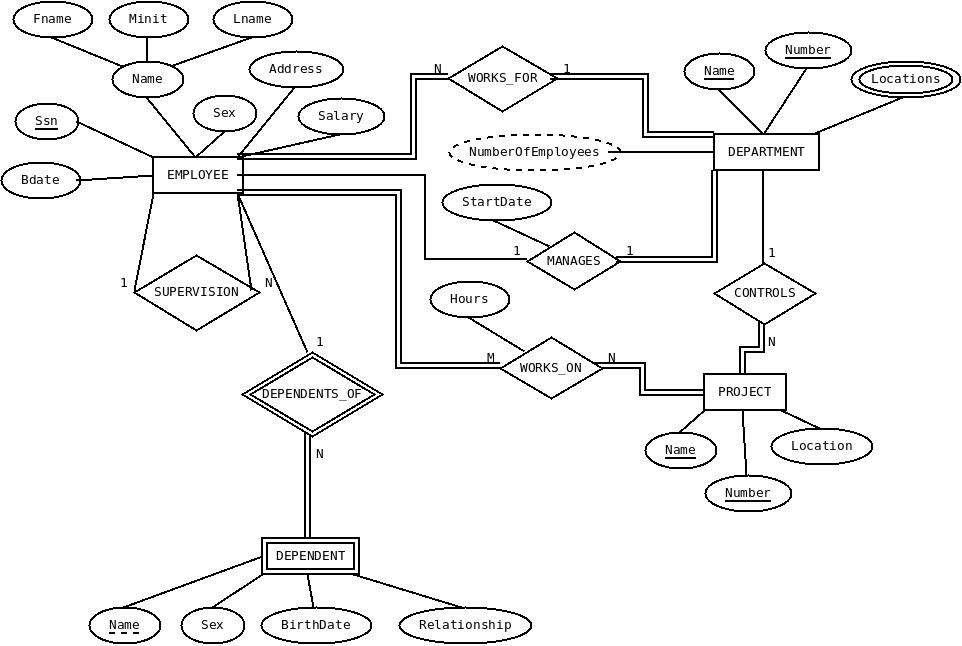
\includegraphics[width=0.6\textwidth]{exemplos/diagramas/ER.jpeg}
    \fonte{Indicar autor original.}
\end{figure}


\begin{figure}
    \centering
    \caption{Exemplo de diagrama - salvo imagem vetorizada - EPS}
    \label{fig:uml_dia_vetorizado_eps}
	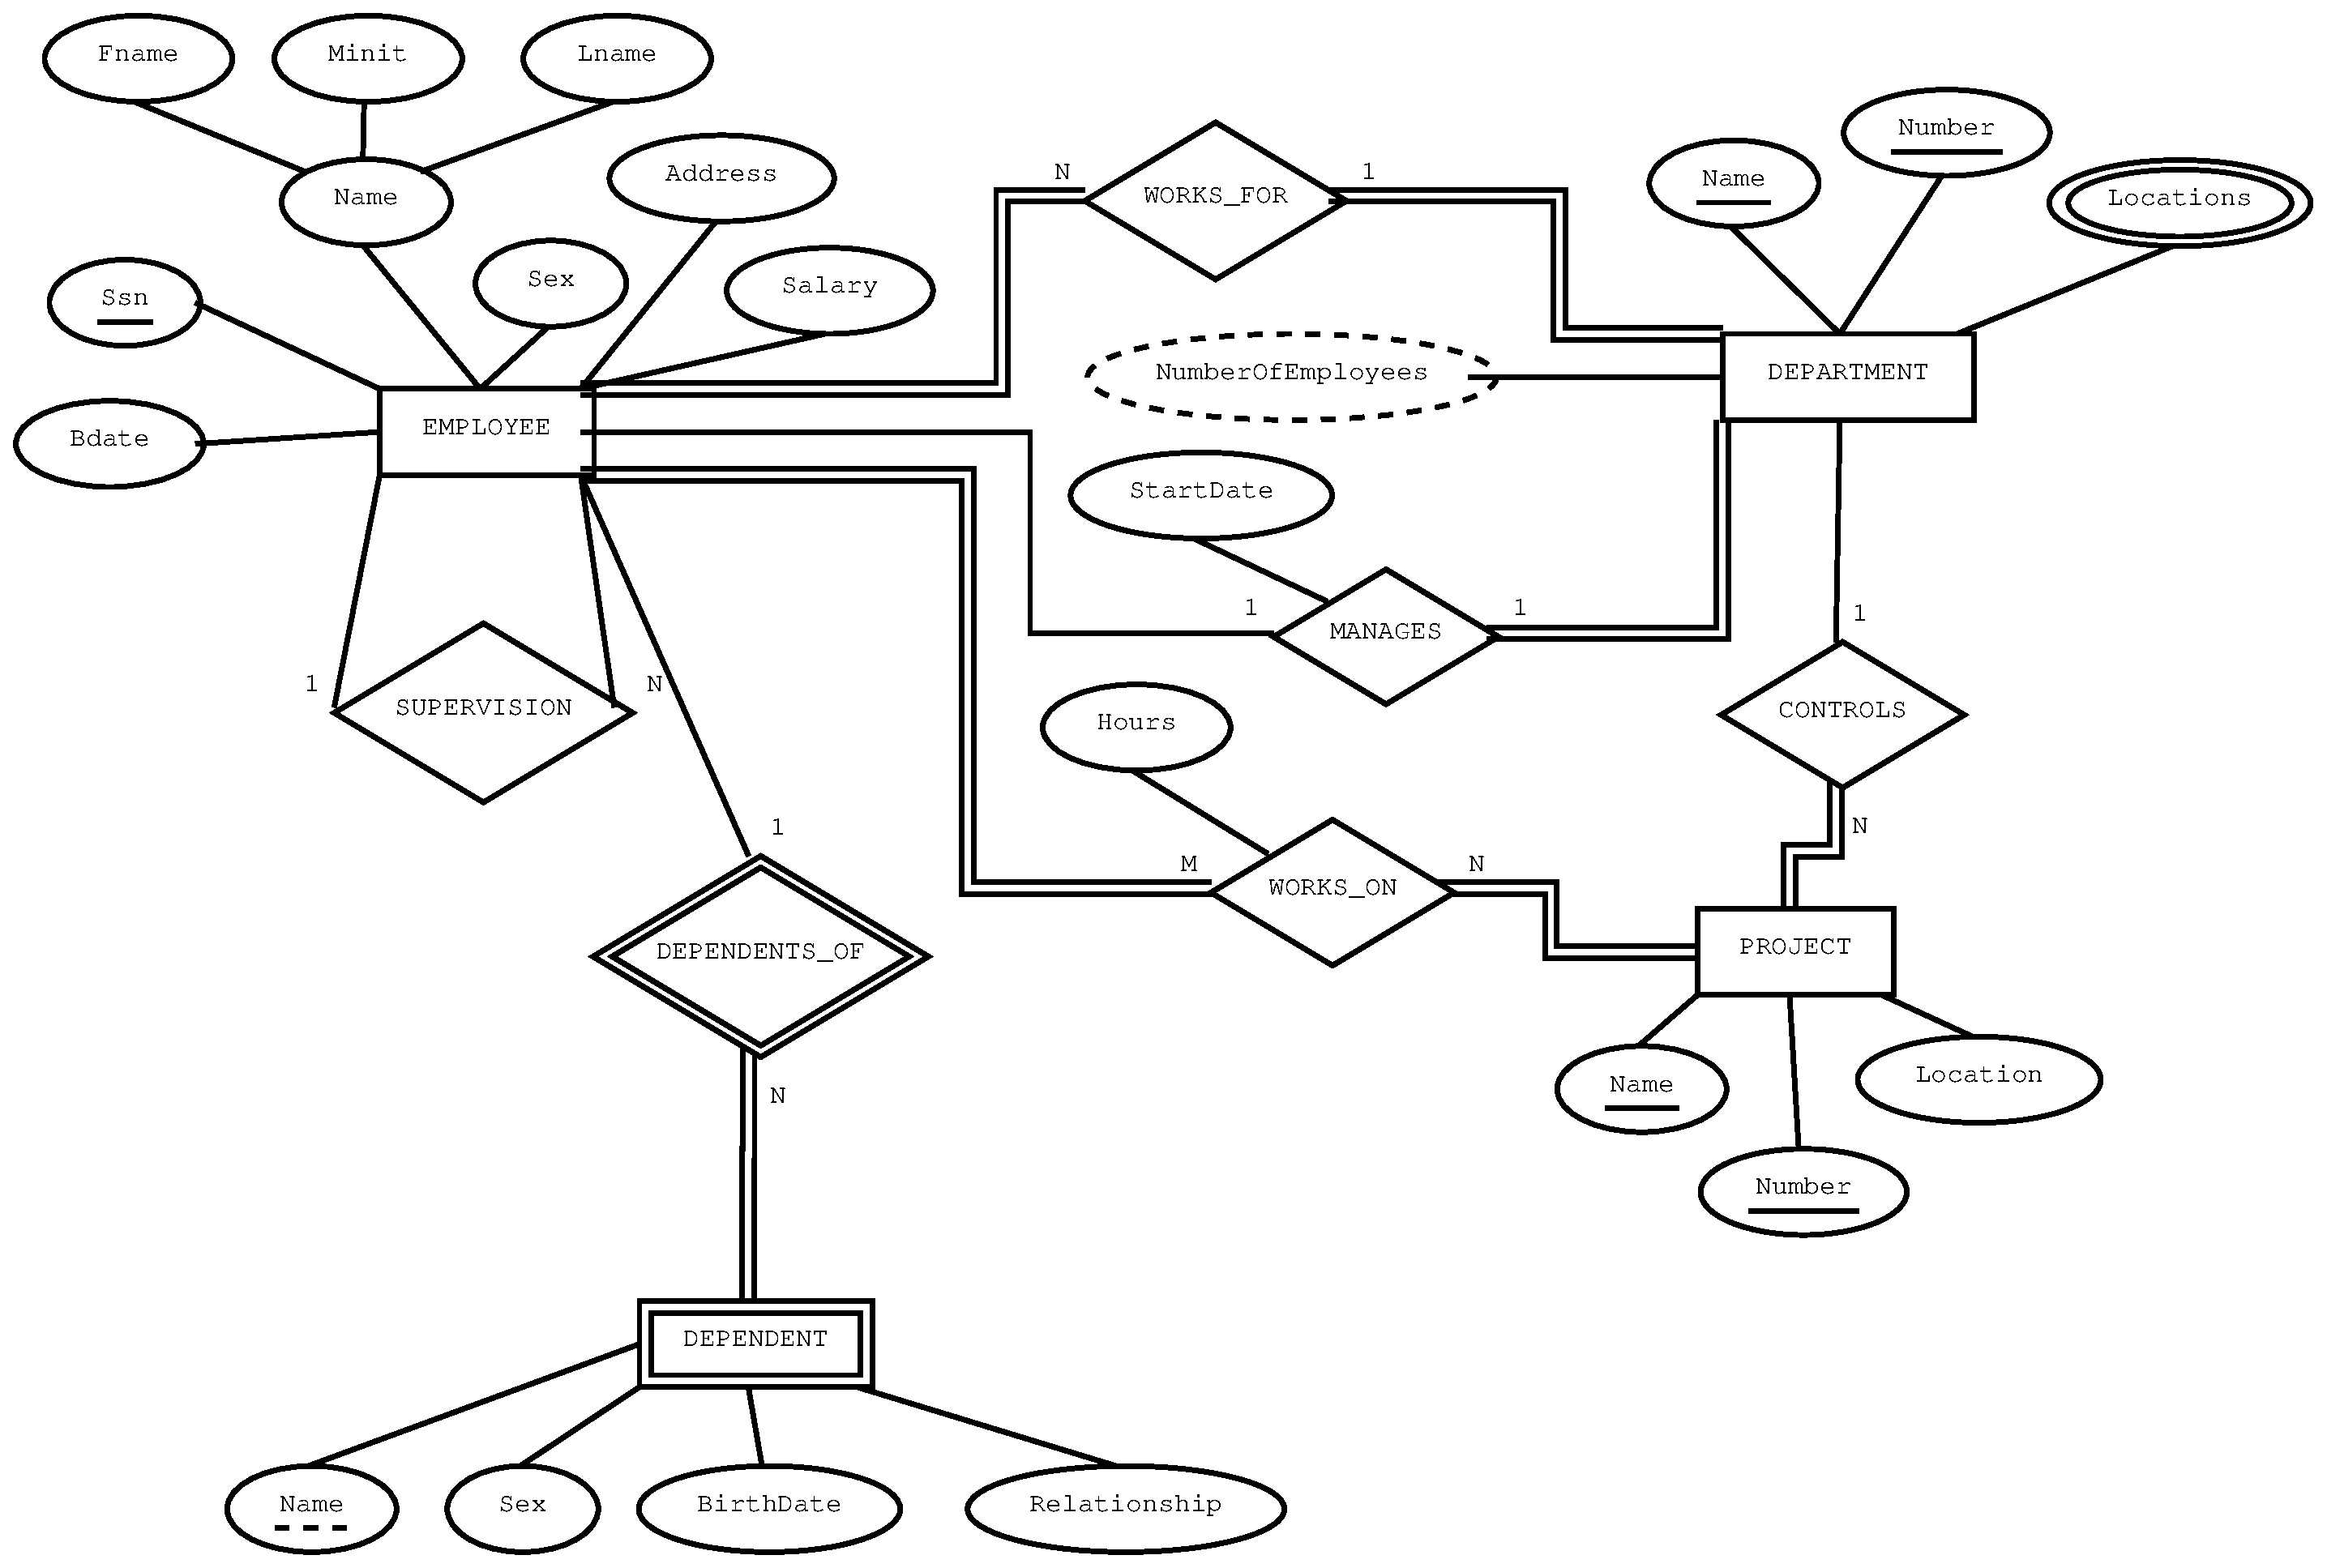
\includegraphics[width=0.6\textwidth]{exemplos/diagramas/ER.eps}
    \fonte{Indicar autor original.}
\end{figure}

\begin{figure}
    \centering
    \caption{Exemplo de diagrama - salvo imagem vetorizada - SVG}
    \label{fig:uml_dia_vetorizado_svg}
    \includesvg[inkscapelatex=false,width=0.6\textwidth]{exemplos/diagramas/ER.svg}
    \fonte{Indicar autor original.}
\end{figure}



% generated by Plantuml 7997beta
\definecolor{plantucolor0000}{RGB}{254,254,206}
\definecolor{plantucolor0001}{RGB}{168,0,54}
\definecolor{plantucolor0002}{RGB}{173,209,178}
\definecolor{plantucolor0003}{RGB}{0,0,0}
\definecolor{plantucolor0004}{RGB}{0,0,255}

\begin{figure}[htb]
    \centering
    \caption{\label{diagramauml}Exemplo de Diagrama UML gerado a partir do PlantUML}
\begin{tikzpicture}[yscale=-1]
\draw[color=plantucolor0001,fill=plantucolor0000,line width=1.5pt] (131pt,29pt) rectangle (223pt,90.8359pt);
\draw[color=plantucolor0001,fill=plantucolor0002,line width=1.0pt] (146pt,45pt) ellipse (11pt and 11pt);
\draw[color=black,fill=black] (148.7656pt,40.875pt) ..controls (148.9219pt,40.6563pt) .. (149.1094pt,40.5469pt) ..controls (149.2969pt,40.4375pt) .. (149.5156pt,40.4375pt) ..controls (149.8906pt,40.4375pt) .. (150.125pt,40.6953pt) ..controls (150.3594pt,40.9531pt) .. (150.3594pt,41.5625pt) -- (150.3594pt,43.0156pt) ..controls (150.3594pt,43.625pt) .. (150.125pt,43.8906pt) ..controls (149.8906pt,44.1563pt) .. (149.5156pt,44.1563pt) ..controls (149.1719pt,44.1563pt) .. (148.9688pt,43.9531pt) ..controls (148.7656pt,43.7656pt) .. (148.6563pt,43.25pt) ..controls (148.6094pt,42.8906pt) .. (148.4219pt,42.7031pt) ..controls (148.0938pt,42.3281pt) .. (147.4844pt,42.1094pt) ..controls (146.875pt,41.8906pt) .. (146.25pt,41.8906pt) ..controls (145.4844pt,41.8906pt) .. (144.8516pt,42.2188pt) ..controls (144.2188pt,42.5469pt) .. (143.7266pt,43.2969pt) ..controls (143.2344pt,44.0469pt) .. (143.2344pt,45.0781pt) -- (143.2344pt,46.1719pt) ..controls (143.2344pt,47.4063pt) .. (144.125pt,48.2266pt) ..controls (145.0156pt,49.0469pt) .. (146.6094pt,49.0469pt) ..controls (147.5469pt,49.0469pt) .. (148.2031pt,48.7969pt) ..controls (148.5938pt,48.6406pt) .. (149.0156pt,48.2031pt) ..controls (149.2813pt,47.9375pt) .. (149.4297pt,47.8594pt) ..controls (149.5781pt,47.7813pt) .. (149.7813pt,47.7813pt) ..controls (150.1094pt,47.7813pt) .. (150.3672pt,48.0391pt) ..controls (150.625pt,48.2969pt) .. (150.625pt,48.6406pt) ..controls (150.625pt,48.9844pt) .. (150.2813pt,49.3906pt) ..controls (149.7813pt,49.9688pt) .. (148.9844pt,50.2969pt) ..controls (147.9063pt,50.75pt) .. (146.6094pt,50.75pt) ..controls (145.0938pt,50.75pt) .. (143.8906pt,50.125pt) ..controls (142.9063pt,49.625pt) .. (142.2188pt,48.5547pt) ..controls (141.5313pt,47.4844pt) .. (141.5313pt,46.2031pt) -- (141.5313pt,45.0469pt) ..controls (141.5313pt,43.7188pt) .. (142.1484pt,42.5703pt) ..controls (142.7656pt,41.4219pt) .. (143.8594pt,40.8047pt) ..controls (144.9531pt,40.1875pt) .. (146.1875pt,40.1875pt) ..controls (146.9219pt,40.1875pt) .. (147.5703pt,40.3516pt) ..controls (148.2188pt,40.5156pt) .. (148.7656pt,40.875pt);
\node at (160pt,37.4531pt)[below right]{Subscriber};
\draw[color=plantucolor0001,line width=1.5pt] (132pt,61pt) -- (222pt,61pt);
\node at (137pt,65pt)[below right]{subscriberId};
\draw[color=plantucolor0001,line width=1.5pt] (132pt,82.8359pt) -- (222pt,82.8359pt);
\draw[color=plantucolor0001,fill=plantucolor0000,line width=1.5pt] (31pt,212pt) rectangle (137pt,273.8359pt);
\draw[color=plantucolor0001,fill=plantucolor0002,line width=1.0pt] (46pt,228pt) ellipse (11pt and 11pt);
\draw[color=black,fill=black] (48.7656pt,223.875pt) ..controls (48.9219pt,223.6563pt) .. (49.1094pt,223.5469pt) ..controls (49.2969pt,223.4375pt) .. (49.5156pt,223.4375pt) ..controls (49.8906pt,223.4375pt) .. (50.125pt,223.6953pt) ..controls (50.3594pt,223.9531pt) .. (50.3594pt,224.5625pt) -- (50.3594pt,226.0156pt) ..controls (50.3594pt,226.625pt) .. (50.125pt,226.8906pt) ..controls (49.8906pt,227.1563pt) .. (49.5156pt,227.1563pt) ..controls (49.1719pt,227.1563pt) .. (48.9688pt,226.9531pt) ..controls (48.7656pt,226.7656pt) .. (48.6563pt,226.25pt) ..controls (48.6094pt,225.8906pt) .. (48.4219pt,225.7031pt) ..controls (48.0938pt,225.3281pt) .. (47.4844pt,225.1094pt) ..controls (46.875pt,224.8906pt) .. (46.25pt,224.8906pt) ..controls (45.4844pt,224.8906pt) .. (44.8516pt,225.2188pt) ..controls (44.2188pt,225.5469pt) .. (43.7266pt,226.2969pt) ..controls (43.2344pt,227.0469pt) .. (43.2344pt,228.0781pt) -- (43.2344pt,229.1719pt) ..controls (43.2344pt,230.4063pt) .. (44.125pt,231.2266pt) ..controls (45.0156pt,232.0469pt) .. (46.6094pt,232.0469pt) ..controls (47.5469pt,232.0469pt) .. (48.2031pt,231.7969pt) ..controls (48.5938pt,231.6406pt) .. (49.0156pt,231.2031pt) ..controls (49.2813pt,230.9375pt) .. (49.4297pt,230.8594pt) ..controls (49.5781pt,230.7813pt) .. (49.7813pt,230.7813pt) ..controls (50.1094pt,230.7813pt) .. (50.3672pt,231.0391pt) ..controls (50.625pt,231.2969pt) .. (50.625pt,231.6406pt) ..controls (50.625pt,231.9844pt) .. (50.2813pt,232.3906pt) ..controls (49.7813pt,232.9688pt) .. (48.9844pt,233.2969pt) ..controls (47.9063pt,233.75pt) .. (46.6094pt,233.75pt) ..controls (45.0938pt,233.75pt) .. (43.8906pt,233.125pt) ..controls (42.9063pt,232.625pt) .. (42.2188pt,231.5547pt) ..controls (41.5313pt,230.4844pt) .. (41.5313pt,229.2031pt) -- (41.5313pt,228.0469pt) ..controls (41.5313pt,226.7188pt) .. (42.1484pt,225.5703pt) ..controls (42.7656pt,224.4219pt) .. (43.8594pt,223.8047pt) ..controls (44.9531pt,223.1875pt) .. (46.1875pt,223.1875pt) ..controls (46.9219pt,223.1875pt) .. (47.5703pt,223.3516pt) ..controls (48.2188pt,223.5156pt) .. (48.7656pt,223.875pt);
\node at (60pt,220.4531pt)[below right]{AccumUsage};
\draw[color=plantucolor0001,line width=1.5pt] (32pt,244pt) -- (136pt,244pt);
\node at (37pt,248pt)[below right]{subscriberId};
\draw[color=plantucolor0001,line width=1.5pt] (32pt,265.8359pt) -- (136pt,265.8359pt);
\draw[color=plantucolor0001,fill=plantucolor0000,line width=1.5pt] (221pt,191pt) rectangle (318pt,294.3438pt);
\draw[color=plantucolor0001,fill=plantucolor0002,line width=1.0pt] (240.05pt,207pt) ellipse (11pt and 11pt);
\draw[color=black,fill=black] (242.8156pt,202.875pt) ..controls (242.9719pt,202.6563pt) .. (243.1594pt,202.5469pt) ..controls (243.3469pt,202.4375pt) .. (243.5656pt,202.4375pt) ..controls (243.9406pt,202.4375pt) .. (244.175pt,202.6953pt) ..controls (244.4094pt,202.9531pt) .. (244.4094pt,203.5625pt) -- (244.4094pt,205.0156pt) ..controls (244.4094pt,205.625pt) .. (244.175pt,205.8906pt) ..controls (243.9406pt,206.1563pt) .. (243.5656pt,206.1563pt) ..controls (243.2219pt,206.1563pt) .. (243.0188pt,205.9531pt) ..controls (242.8156pt,205.7656pt) .. (242.7063pt,205.25pt) ..controls (242.6594pt,204.8906pt) .. (242.4719pt,204.7031pt) ..controls (242.1438pt,204.3281pt) .. (241.5344pt,204.1094pt) ..controls (240.925pt,203.8906pt) .. (240.3pt,203.8906pt) ..controls (239.5344pt,203.8906pt) .. (238.9016pt,204.2188pt) ..controls (238.2688pt,204.5469pt) .. (237.7766pt,205.2969pt) ..controls (237.2844pt,206.0469pt) .. (237.2844pt,207.0781pt) -- (237.2844pt,208.1719pt) ..controls (237.2844pt,209.4063pt) .. (238.175pt,210.2266pt) ..controls (239.0656pt,211.0469pt) .. (240.6594pt,211.0469pt) ..controls (241.5969pt,211.0469pt) .. (242.2531pt,210.7969pt) ..controls (242.6438pt,210.6406pt) .. (243.0656pt,210.2031pt) ..controls (243.3313pt,209.9375pt) .. (243.4797pt,209.8594pt) ..controls (243.6281pt,209.7813pt) .. (243.8313pt,209.7813pt) ..controls (244.1594pt,209.7813pt) .. (244.4172pt,210.0391pt) ..controls (244.675pt,210.2969pt) .. (244.675pt,210.6406pt) ..controls (244.675pt,210.9844pt) .. (244.3313pt,211.3906pt) ..controls (243.8313pt,211.9688pt) .. (243.0344pt,212.2969pt) ..controls (241.9563pt,212.75pt) .. (240.6594pt,212.75pt) ..controls (239.1438pt,212.75pt) .. (237.9406pt,212.125pt) ..controls (236.9563pt,211.625pt) .. (236.2688pt,210.5547pt) ..controls (235.5813pt,209.4844pt) .. (235.5813pt,208.2031pt) -- (235.5813pt,207.0469pt) ..controls (235.5813pt,205.7188pt) .. (236.1984pt,204.5703pt) ..controls (236.8156pt,203.4219pt) .. (237.9094pt,202.8047pt) ..controls (239.0031pt,202.1875pt) .. (240.2375pt,202.1875pt) ..controls (240.9719pt,202.1875pt) .. (241.6203pt,202.3516pt) ..controls (242.2688pt,202.5156pt) .. (242.8156pt,202.875pt);
\node at (254.95pt,199.4531pt)[below right]{IpSession};
\draw[color=plantucolor0001,line width=1.5pt] (222pt,223pt) -- (317pt,223pt);
\node at (227pt,227pt)[below right]{ipAddress};
\node at (227pt,240.8359pt)[below right]{specificData};
\node at (227pt,254.6719pt)[below right]{sapcOriginStateId};
\node at (227pt,268.5078pt)[below right]{apnId};
\draw[color=plantucolor0001,line width=1.5pt] (222pt,286.3438pt) -- (317pt,286.3438pt);
\draw[color=plantucolor0004] (191.942pt,90.081pt) ..controls (205.204pt,115.893pt) and (224.952pt,154.325pt) .. (241.265pt,186.076pt);
\draw[color=plantucolor0004,fill=plantucolor0004] (243.646pt,190.709pt) -- (243.0894pt,180.8759pt) -- (241.3604pt,186.262pt) -- (235.9742pt,184.5329pt) -- (243.646pt,190.709pt) -- cycle;
\node at (191.0584pt,98.9168pt)[below right]{1};
\node at (230.3817pt,166.6703pt)[below right]{1..*};
\draw[color=plantucolor0001] (162.058pt,90.081pt) ..controls (145.645pt,122.023pt) and (119.302pt,173.295pt) .. (101.824pt,207.31pt);
\draw[color=plantucolor0001,fill=plantucolor0001] (99.5252pt,211.784pt) -- (107.1969pt,205.6078pt) -- (101.8108pt,207.337pt) -- (100.0816pt,201.9509pt) -- (99.5252pt,211.784pt) -- cycle;
\node at (143.0082pt,98.7264pt)[below right]{1};
\node at (101.801pt,187.522pt)[below right]{0..1};
\end{tikzpicture}
	\legend{Fonte: Exemplos PlantUML.}
\end{figure}

A \autoref{fig_diag_virado} exemplifica como utilizar uma imagem em formato paisagem (página inteira). Obs: Utilizamos propositalmente uma imagem não vetorizada de forma a ilustrar o procedimento e também para apresentar que a qualidade não fica boa o suficiente para leitura. Uma versão vetorizada dessa figura teria qualidade melhor.


% observe que a imagem a seguir teve que ser ajustada para caber corretamente na página
% por não ser uma imagem vetorizada a qualidade não é a melhor possivel
\begin{sidewaysfigure}[htb]
    \centering
	\caption{\label{fig_diag_virado}Diagrama Virado - Exemplo}
	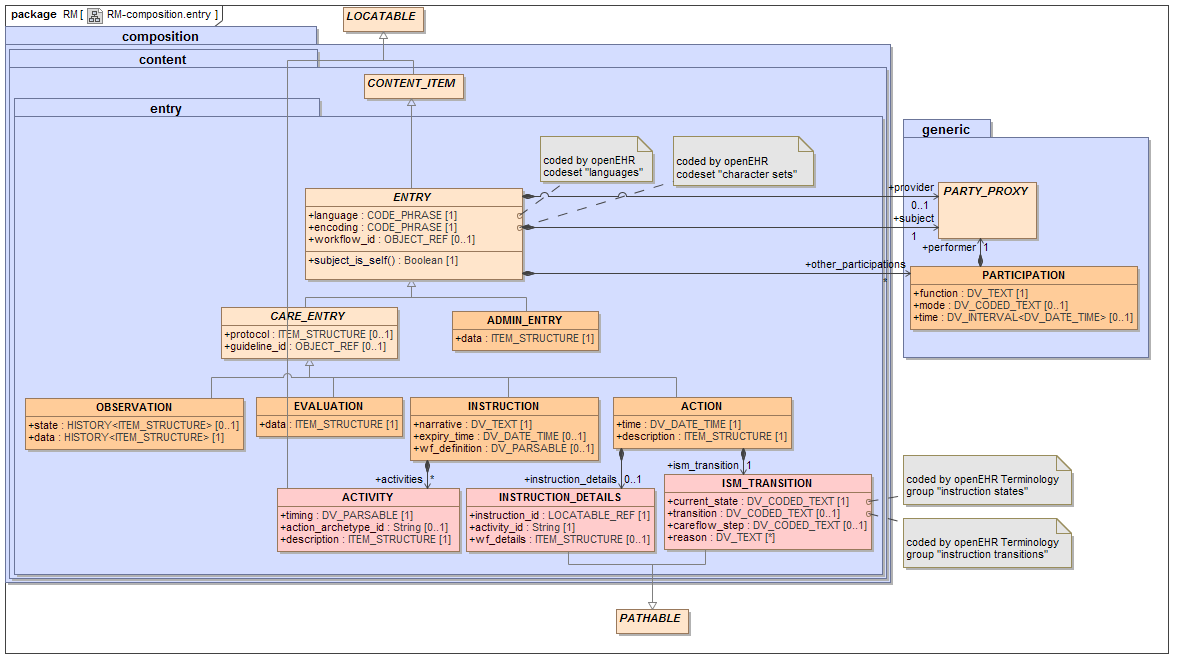
\includegraphics[width=0.9\textwidth]{exemplos/exemplo_diag_horizontal.png}
	\fonte{\citeonline{openehrCompositionEntry}.}
\end{sidewaysfigure}


\subsection{Impressão em folhas formato A3}

A página seguinte em A3 permite a impressão de diagramas grandes que não podem ser visualizados facilmente em folha padrão A4. Lembre que algumas impressoras podem ter problemas com isso, então selecione somente as páginas A4 ao imprimir e depois imprima separadamente a página A3.

A \autoref{fig_logo_A3} utiliza a mesma imagem da \autoref{fig_logo} e foi ampliada para demonstrar a essa possibilidade de impressão de grandes imagens em A3.

Observe que o código de exemplo vai gerar uma quebra de página no local onde for definida a página A3, por isso não deve ser utilizado entre textos para evitar grandes espaços em branco.

Folhas impressas em A3 ou tamanhos maiores devem ser dobradas seguindo o padrão definido pela \ac{abnt}. 


Cuidado ao utilizar folhas A3 em um documento impresso em frente e verso pois a numeração das páginas seguintes pode ser impressa de forma incorreta (posição do número na página). Uma alternativa para esta situação é manter todas páginas impressas em A3 no último apêndice, fazendo as referencias corretas durante o texto.



 \afterpage{%
 \begin{PAGINA-A3}

 \begin{figure}[p]
     \centering%
 	\caption{\label{fig_logo_A3}Logotipo \acs{ifsp} em página A3}
     \fcolorbox{red}{yellow}{ 
\includegraphics[height=\textheight,width=\textwidth,keepaspectratio]{\ifspprefixo/logo-02.jpg}}%
 	\legend{Com borda para demonstrar os limites}
   \fonte{citar o autor da Figura(xxx).}
 \end{figure}

 \end{PAGINA-A3}
 }


%%
% Macros para simplificar a demonstração dos erros
%

\newcommand{\errado}[1]{\textbf{\textcolor{red}{#1}}}
\newcommand{\certo}[1]{\textbf{\textcolor{ForestGreen}{#1}}}
% Para não confundir com os exemplos de certo e errado não são colocados os pontos e ponto e virgula dos itens
\newcommand{\erradocerto}[3]{\item #1:\begin{itemize}
    \item \errado{#2}
    \item \certo{#3}
\end{itemize}}
\newcommand{\erradoerradocerto}[4]{\item #1:\begin{itemize}
    \item \errado{#2}
    \item \errado{#3}
    \item \certo{#4}
\end{itemize}}
\newcommand{\erradocertocerto}[4]{\item #1:\begin{itemize}
    \item \errado{#2}
    \item \certo{#3}
    \item \certo{#4}
\end{itemize}}



% Para demonstrar o erro nome deve ser igual entre o capitulo e a seção, então fica em um comando para facilitar
\newcommand{\nomeDoCapitulo}{Erros comuns em documentos}
\chapter{\nomeDoCapitulo}
\label{erros-comuns-capitulo}

% Não colocar nada aqui pois é uma demonstração de erro comum
\explicacaoErro{Passando de capítulo para seção sem texto}
\explicacaoErro{Seção com mesmo nome do capítulo}

\section{\nomeDoCapitulo}
\label{erros-comuns}

% Não colocar nada aqui pois é uma demonstração de erro comum
\explicacaoErro{Passando de seção para subseção sem texto}

\subsection{Subseção sem texto entre o item anterior}
\label{erros-comuns-sub1}


% Tem um erro proposital aqui duplicando "seção" que é escrita também pelo autoref, esse erro é citado em um paragrafo na sequencia....
Essa seção \autoref{erros-comuns} demonstra alguns dos erros mais comuns que percebemos em trabalhos de alunos. Alguns itens errados são apresentados em \errado{vermelho} e corretos em \certo{verde}, mas devido a formatação dos links pode haver uma variação. Lembre que a utilização de cores não é recomendada no documento acadêmico, elas foram utilizadas nesse documento para facilitar a demonstração dos erros.

Além desses erros é comum encontrar a falta de correção ortográfica e utilização errada de palavras. É importante sempre utilizar a correção ortográfica e ainda fazer a revisão por diversas pessoas para evitar erros de português, a língua portuguesa tem palavras parecidas com sentidos diferente, cuidado com a utilização dos acentos e pontuação como pode ser visto claramente em  \autoref{fig_portugues_amador}.

No \autoref{revisao-de-textos} é apresentado um processo simples para revisão de documentos que detecta a maior parte dos erros descritos neste documento.

% erro proposital que esta no inicio da seção
Você percebeu que essa seção iniciou com um erro e que esse erro não está indicado em vermelho ?


\begin{figure}[htb]
    \centering
	\caption{\label{fig_portugues_amador}Português não é para amador}
	\frame{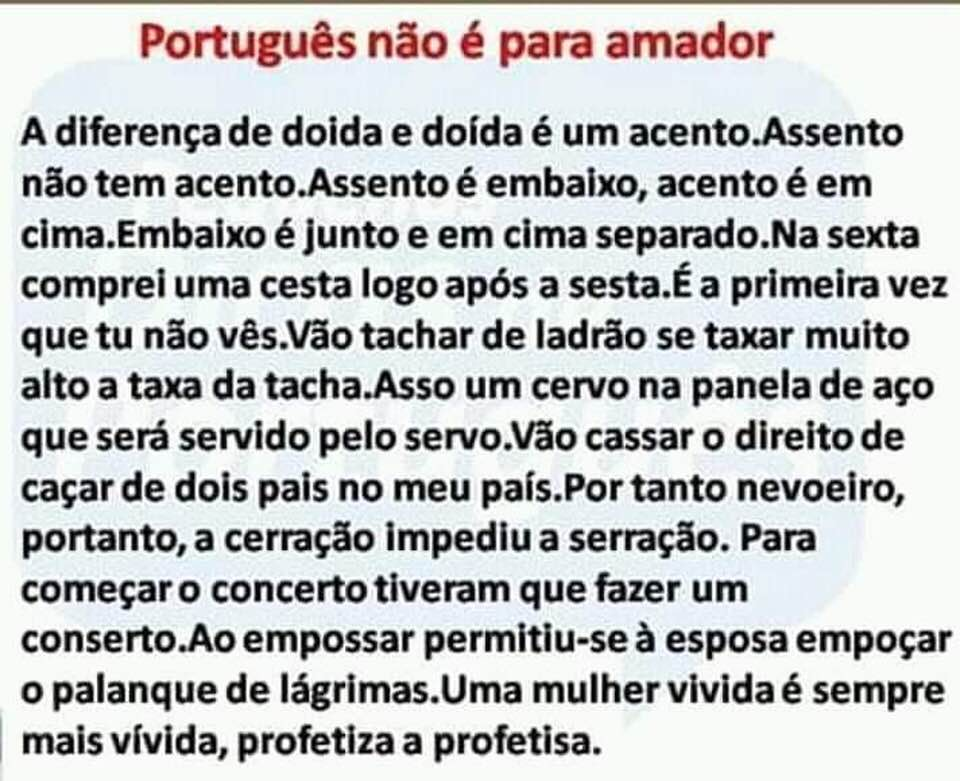
\includegraphics[width=0.9\textwidth]{erros/portugues_nao_eh_para_amador.jpg}}
	\fonte{Autor Desconhecido.}
\end{figure}


Exemplos de erros encontrados em documentos das disciplinas de projetos são apresentados nas seções seguintes. E existem dicas adicionais sobre textos disponíveis em \url{https://dicas.ivanfm.com/aulas/textos/}.


\todo[inline]{Separar esses itens em grupos mais específicos}

\subsection{Subseção com titulo que tenta ser introdução:}
\label{erros-titulo-dois-pontos}
\errado{Colocar um título de seção/seção com dois pontos no final tentando indicar uma introdução para o texto da seção.}
\explicacaoErro{Além disso essa seção tem somente um pequeno parágrafo, ver \autoref{erros-formatacao-docto}}

\subsection{Erros comuns de texto}
    
\begin{itemize}
    \erradocerto{Abreviação ou nomes incompletos dos participantes do trabalho e/ou professores na capa do documento}{Cebolácio Silva}{Cebolácio Júnior Menezes da Silva}

    \erradocerto{Falta de prontuário completo do estudante na capa do documento }{Magali Fernandes de Lima   123456}{Magali Fernandes de Lima    SP123456}

    \item cada parágrafo deve descrever uma ideia então cuidado ao escrever um parágrafo grande demais com diversas ideias envolvidas ou escrever diversos parágrafos pequenos para a mesma ideia; 
        
    \erradocerto{não utilizar palavras em português onde for possível}{o dispositivo mobile}{o dispositivo móvel}

    \erradocerto{não utilizar melhores palavras, algumas palavras chegaram a ser incorporadas a língua portuguesa mas existem palavras melhores e que podem ser utilizadas e as vezes com resultado mais claro}{postagem / deletar / customizar}{publicação / excluir / personalizar}

    \erradocerto{Utilização do tempo verbal incorreto, a escrita do documento muitas vezes inicia antes da finalização, mas o leitor recebe o documento depois do trabalho finalizado}{será desenvolvido - será apresentado}{foi desenvolvido - é apresentado}

    \erradoerradocerto{Referenciar elementos indicando posição, acima, abaixo, a seguir }{... como poder ser visto na Figura abaixo ...}{... como pode ser visto no quadro a seguir ....}{... como pode ser visto na \autoref{fig_portugues_amador} ...}

    \erradocerto{não representar as unidades de forma correta}{3,20 ghz}{3,20 GHz}

    \erradocerto{não ser consistente com os formatos e precisões}{o primeiro tem \textit{clock} de 3,20 GHz e o segundo de 1,8 GHz}{o primeiro tem \textit{clock} de 3,20 GHz e o segundo de 1,80 GHz}
        
    \erradocerto{Escrever as mesmas palavras, com o mesmo sentido de diversas formas diferentes. Um exemplo é o nome de uma empresa famosa em alguns desenhos: ACME}{ACME Corporation é uma sociedade fictícia que existe no universo dos filmes e animações \newline ... \newline A companhia acme reapareceu num desenho animado do Hortelino Troca-Letras com um kit para aprender boxe por correspondência \newline ... \newline Os produtos Acme podem ser encomendados somente pelo correio}{ACME Corporation é uma sociedade fictícia que existe no universo dos filmes e animações \newline ... \newline A companhia ACME reapareceu num desenho animado do Hortelino Troca-Letras com um kit para aprender boxe por correspondência \newline ... \newline Os produtos ACME podem ser encomendados somente pelo correio}
    
\end{itemize}

\subsection{Erros comuns relacionados a formatação do texto e do documento}
\label{erros-formatacao-docto}

\begin{itemize}
    \item \errado{passagem de um item para outro sem texto} como é possível observar entre  \autoref{erros-comuns-capitulo} e \autoref{erros-comuns} e também entre \autoref{erros-comuns} e \autoref{erros-comuns-sub1};
    
    \item \errado{itens com pouco texto} observe que as seções 
    \ref{erros-titulo-dois-pontos}, \ref{erros-comuns-sub-pequena1} e a \ref{erros-comuns-sub-pequena2} possuem pouco texto, cada item deve ter um volume de texto que justifique sua existência, caso o volume de texto seja pequeno agrupe as seções em uma única seção com mais parágrafos;
        
    \item \errado{utilizar o mesmo nome para seções / capítulos como \autoref{erros-comuns-capitulo} e \autoref{erros-comuns}};
        
    \item definições de referências incompletas, a referência \citeonline{ETAL4} está definida faltando cidade, observe que na lista de referencias aparece \errado{[S.l.]} que indica Sem Local, pois a \ac{abnt} exige a indicação de local para livros;

    \erradocerto{incluir dentro do seu texto um documento ou manual que pode ser referenciado e facilmente acessado pelo leitor, faça a citação correta referenciando o documento original}{segundo a \ac{ldb}, a educação brasileira é dividida em dois níveis: a educação básica e o ensino superior}{segundo a \ac{ldb} 9394/96 \cite{ldb}, a educação brasileira é dividida em dois níveis: a educação básica e o ensino superior}
    
    \erradocerto{citação de elementos errados}{Segundo o anexo com o manual pdfpages (\autoref{manual-todonotes}), o comando \mostraComandoLaTeX{includepdf} permite que você faça a inclusão de páginas de documentos externos no seu documento}{Segundo o anexo com o manual pdfpages (\autoref{manual-pdfpages}), o comando \mostraComandoLaTeX{includepdf} permite que você faça a inclusão de páginas de documentos externos no seu documento}
    
    \item \errado{forçar manualmente quebra de página}, o texto deve seguir utilizando todo o espaço disponível nas páginas, o {\LaTeX} faz isso automaticamente, não é necessário forçar uma quebra de página;
    
    \item \errado{não seguir as dicas de revisão} - ver \autoref{revisao-de-textos};
    
    \item \errado{não formatar corretamente tabelas} como indicado na \autoref{sub-erros-tabelas}.

    
\end{itemize}





\subsection{Erros comuns no uso do \LaTeX}

O \LaTeX\ é uma linguagem onde você define o texto e comandos e o resultado da compilação é um arquivo formatado normalmente no formato \ac{pdf}. Com isso algumas características dessa linguagem devem ser consideradas ao escrever seu texto para não cair em alguns problemas já conhecidos:

\begin{itemize}
    \erradocerto{ignorar que após uma macro pode ser necessário incluir um espaço forçado (observe pelo código fonte as diversas maneiras utilizadas para fazer corretamente)}{o \LaTeX permite...}{o \LaTeX\ permite...\newline o {\LaTeX} permite...\newline o \LaTeX \space permite...}

    \erradocertocerto{erro ao definir elementos com aspas, observe que dependendo da forma utilizada o texto fica \enquote{grudado} (observe no código fonte as diferenças)}{"entre aspas" após as aspas}{"entre aspas" \space após as aspas}{\enquote{entre aspas} após as aspas}

    \erradocerto{não utilizar o sistema de siglas / glossário para definições especificas (as definições corretas ficam como links no arquivo final \acs{pdf}), ver \autoref{siglas-glossario}}{IFSP}{\acs{ifsp}}
    
    \erradocerto{Não utilizar a definição de plural do glossário e fazer um plural manualmente}{\gls{crud}s - utilizando a sigla seguida do s para plural}{\glspl{crud} utilizando a definição de plural do glossário}
    
\end{itemize}


\subsection{Subseção com texto pequeno 1}
\label{erros-comuns-sub-pequena1}
\errado{Uma frase única indicando basicamente o que o título da seção é}.

\subsection{Subseção com texto pequeno 2}
\label{erros-comuns-sub-pequena2}
\errado{Mais um paragrafo único indicando basicamente o que o título da seção é, provavelmente isso poderia ir para o glossário, ver \autoref{siglas-glossario}}, uma regra simples para seguir é \certo{se uma seção não tiver pelo menos 3 (três) parágrafos, provavelmente essa informação não precisa de uma seção especifica e pode fazer parte de outra seção}

\subsection{Erros no uso de Ilustrações}
\label{sub-erros-ilustrações}

Ilustrações são elementos não textuais que ajudam na apresentação de informação como Figuras, Quadros e Tabelas.


\begin{itemize}

    \item \errado{utilização de páginas em formato paisagem ou em formato A3 sem necessidade}, antes de fazer isso tente reorganizar as ilustrações para caberem na página no formato padrão (ex um quadro que tem muitas colunas, pode ser alterado para que as colunas virem linhas e dessa forma caber na página em formato padrão);
    
    \erradocerto{não referenciar uma ilustração no texto, toda ilustração deve ser referenciada no texto}{(...)parecidas com sentidos diferente, cuidado com a utilização dos acentos e pontuação como pode ser visto abaixo.}{(...)parecidas com sentidos diferente, cuidado com a utilização dos acentos e pontuação como pode ser visto claramente em \autoref{fig_portugues_amador}}
    
    \erradocerto{não referenciar ilustrações da forma correta, observe que não é somente a questão de maiúscula/minúscula mas também o link que inclui o tipo de ilustração}{a tabela \ref{tabela-correta-equipamento} ...}{a \autoref{tabela-correta-equipamento} ...}
    
    \erradoerradocerto{não referenciar corretamente sequencias de ilustrações, esse caso pode até dar a impressão de inconsistência com o caso anterior}{nas \autoref{tab-exemplo} até \autoref{tabela-correta-servicos}}{nas Tabelas de  \autoref{tab-exemplo} até \autoref{tabela-correta-servicos}}{nas Tabelas de \ref{tab-exemplo} até \ref{tabela-correta-servicos} \newline a partir da \autoref{tab-exemplo} até a \autoref{tabela-correta-servicos}}

    \erradocerto{deixar referencia jogada sem fazer parte do texto}{durante o projeto foram registradas as métricas. \autoref{tabela-correta-servicos}}{a \autoref{tabela-correta-servicos} apresenta os valores das métricas levantadas durante o projeto.}

    \item \errado{\enquote{estourar} a margem do documento, como na \autoref{tabela-errada}};
    
    \erradoerradocerto{indicar a ferramenta utilizada como fonte de ilustração}{Fonte: Trello}{Fonte: Excel}{Fonte: Os Autores}
    
    \item \errado{repetir a mesma ilustração em dois locais no documento, a figura não deve ser repetida, mas referenciada novamente};

    \item \errado{não utilizar imagens vetorizadas} para obter a melhor qualidade, ver \autoref{sec_figuras};

    \item \errado{utilização de cores em um documento que vai ser impresso em preto e branco};

    \item \errado{tentar posicionar ilustrações em locais específicos} (ex abaixo do texto), o correto é referenciar a ilustração no texto e deixar o \LaTeX\ posicionar de acordo com a disponibilidade de espaço no documento, mas você deve recomendar que o local da definição seja prioritário, ver \autoref{elementos-nao-textuais}. Se as suas imagens ficam distantes do texto onde foram referenciadas provavelmente você não descreveu de forma suficiente as ilustrações ou você precisa de mais texto condizente no seu documento;
    
    \item \errado{ilustrações muito distantes do local onde foram citadas}, o {\LaTeX} ajusta o posicionamento das ilustrações automaticamente, você deve colocar a definição próximo do local da citação e não ficar forçando quebras de páginas. Se suas ilustrações estão ficando longe da referencia significa que você tem pouco texto e com isso as ilustrações ficam distantes. Em alguns casos uma opção pode ser utilizar os apêndices para conjuntos grandes de ilustrações deixando o texto principal mais organizado, além disso esse modelo possui um comando \mostraComandoLaTeX{autorefWithPage} que pode auxiliar em alguns casos onde for necessário referenciar uma ilustração que fique posicionada distante do local de citação.
\end{itemize}

Os nomes que definimos para as ilustrações devem ser claros o bastante para permitir que o leitor os identifique nas listas no inicio do documento. A \autoref{fig_erros_lista_quadros} apresenta um trecho de uma lista de quadros com dois problemas encontrados em trabalhos :

\begin{itemize}
    \erradocerto{Repetição de nomes em elementos diferentes}{é possível observar que existem dois quadros com nome \textbf{Caso de Uso 10} na \autoref{fig_erros_lista_quadros}}{Cada elemento deve ter um nome próprio}

    \erradocerto{Utilização de nomes que não são claros para cada elemento}{Caso de Uso 07}{Caso de Uso 07 - Recuperação de senha}.
    
    \erradocerto{Nomes que não indicam claramente o conteúdo da ilustração como é possível observar na \autoref{fig_erros_lista_quadros_2}}{Quadro X - Usuário}{Quadro X - Dicionário de dados - Entidade Usuário}
\end{itemize}


\begin{figure}[htb]
    \centering
	\caption{\label{fig_erros_lista_quadros}Exemplo de Lista de quadros com erros comuns (Casos de uso)}
	\frame{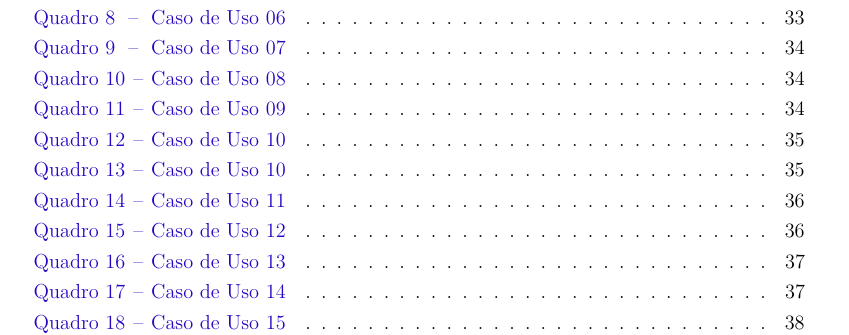
\includegraphics[width=0.9\textwidth]{erros/erros_lista_quadros.png}}
    \fonte{Trecho de um trabalho com o erro (omitida autoria propositadamente).}
\end{figure}

\begin{figure}[htb]
    \centering
	\caption{\label{fig_erros_lista_quadros_2}Exemplo de Lista de quadros com erro nos títulos}
	\frame{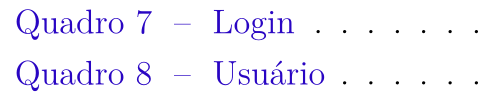
\includegraphics{erros/quadros_login_usuario.png}}
    \fonte{Trecho de um trabalho com o erro (omitida autoria propositadamente).}
\end{figure}



\subsection{Erros em tabelas e quadros}
\label{sub-erros-tabelas}
A \autoref{tabelas-e-quadros} demonstra como devemos formatar corretamente tabelas e quadros (e também indica quando devemos utilizar cada tipo de ilustração), a \autoref{tabela-errada} mostra diversos erros comuns que encontramos em tabelas e quadros, e as Tabelas \ref{tabela-correta-equipamento} e \ref{tabela-correta-servicos} mostram os mesmos dados apresentados de uma forma correta. Uma tabela formatada corretamente permite a leitura e comparação dos dados de forma mais fácil. Observe a lista de erros da \autoref{tabela-errada} :


\begin{itemize}
    \item \errado{formatação de bordas como um quadro e não como tabela};

    \item \errado{títulos sem negrito dificultando a sua leitura e identificação};
    
    \item \errado{não limitar tamanho de coluna que tem dados grandes de forma a estourar o espaço disponível};
    
    \item \errado{números não estão alinhados a direita};
    
    \item \errado{itens sem ordem especifica}, \certo{os itens devem vir em uma ordem lógica ou ordem alfabética};
    
    \item \errado{inconsistência de precisão, em uma célula o valor tem duas casas decimais e em outras não possuem casas decimais};
    
    \item \errado{mistura de dados de situações diferentes (ex: custo único e custo mensal sem normalização)};
    
    \item \errado{repetição do R\$ mesmo tendo ele no título da coluna}.
\end{itemize}

% Essa tabela além dos erros na colocação dos dados também está "estourando" a margem pois não está quebrando o texto um caso muito comum nos documentos que recebemos... 
\begin{table}[thb]
\centering
\ABNTEXfontereduzida
\caption{Valores de equipamentos (formação de forma errada e passando da margem)}
\label{tabela-errada}
\begin{tabular}{|l|c|l|l|}
\hline
Equipamento/Serviço & Valor Unitário R\$ & Quantidade & Valor Total R\$ \\ \hline
Teclado     & R\$60          & 2          & R\$120     \\ \hline
Monitor     & R\$:600          & 2          & R\$ 1200,00     \\ \hline
Internet     & R\$220          & 1          & R\$ 220     \\ \hline
Texto muito muito grande que deveria ser quebrado   & R\$120          & 1          & R\$ 120     \\ \hline
\end{tabular}
	\fonte{Os Autores.}
\end{table}

\begin{table}[]
\centering
\ABNTEXfontereduzida
\caption{Valores de equipamentos - Compra (formatada corretamente)}
\label{tabela-correta-equipamento}
\begin{tabular}{p{5.0cm}rrr}
\hline
\thead{Equipamento} & \thead{Valor\\Unitário\\R\$} & \thead{Quantidade} & \thead{Valor\\Total\\ R\$} \\ \hline
Monitor     & 600,00          & 2          & 1200,00     \\ 
Teclado     & 60,00          & 2          & 120,00     \\ 
Texto muito muito grande que deveria ser quebrado     & 220,00          & 1          & 220,00     \\ 
\hline
\textbf{TOTAL} & & & 1540,00 \\
\hline
\end{tabular}
\fonte{Os autores.}
\end{table}

\begin{table}[]
\centering
\ABNTEXfontereduzida
\caption{Valores de equipamentos - Mensal (formatada corretamente)}
\label{tabela-correta-servicos}
\begin{tabular}{lrrr}
\hline
\thead{Serviço} & \thead{Valor Unitário R\$} & \thead{Quantidade} & \thead{Valor Mensal R\$} \\ \hline
Internet     & 120,00          & 1          & 120,00     \\ \hline
\end{tabular}
\fonte{Os autores.}
\end{table}

Também é necessário cuidado em termos de formatação das ilustrações em termos de consistência e quebras :

\begin{itemize}
    
    \item \errado{quadros que devem representar o mesmo tipo de informação com formatação diferente}, uma maneira simples de garantir a padronização da formatação é utilizar o recurso de criação de comandos no {\LaTeX}, dessa forma todos elementos serão apresentados de forma consistente;

    \item \errado{utilização de \index{longtable}longtable sem necessidade} quebrando um quadro ou tabela que poderia ser apresentado em uma única página, quando o quadro ou tabela for maior que uma página a melhor maneira é quebrar em quadros que agrupem as informações de forma consistente.

\end{itemize}

\todo[inline]{gerar figura demonstrando erro do longtable com tabelas pequenas que ficam quebradas em diferentes páginas}    


Em quadros pequenos detalhes podem fazer uma grande diferença na apresentação de informação, como pode ser observado nos Quadros \ref{quadro-poluido},  \ref{quadro-poluido-limpo-desalinhado} e \ref{quadro-poluido-limpo} :

\begin{itemize}
    \item \errado{O \autoref{quadro-poluido} foi montado com textos que não facilitam a leitura};
    
    \item \errado{O \autoref{quadro-poluido-limpo-desalinhado} teve uma melhora mas sem centralização das informações};

    \item \certo{O \autoref{quadro-poluido-limpo} apresenta a mesma informação do de forma mais limpa e facilitando a leitura}.
\end{itemize}



\begin{quadro}[thb]
\centering
\ABNTEXfontereduzida
\caption{Distribuição de Atividades (poluído, difícil de ler) }
\label{quadro-poluido}
\begin{tabular}{|l|c|c|c|c|}
\hline
\thead{Responsável} & \thead{Atividade 1} & \thead{Atividade 2} & \thead{Atividade 3} & \thead{Atividade 4} \\
\hline
%
Pessoa 1 & SIM         & NÃO         & NÃO         & SIM         \\
\hline
Pessoa 2 & SIM         & NÃO         & SIM         & NÃO         \\
\hline
Pessoa 3 & NÃO         & SIM         & NÃO         & NÃO         \\
\hline
Pessoa 4 & NÃO         & SIM         & SIM         & NÃO        \\
\hline
\end{tabular}
\fonte{Os autores.}
\end{quadro}


\begin{quadro}[thb]
\centering
\ABNTEXfontereduzida
\caption{Distribuição de Atividades (sem centralização)}
\label{quadro-poluido-limpo-desalinhado}
\begin{tabular}{|l|l|l|l|l|}
\hline
\thead{Responsável} & \thead{Atividade 1} & \thead{Atividade 2} & \thead{Atividade 3} & \thead{Atividade 4} \\
\hline
Pessoa 1 & \circlemark       &          &             & \circlemark         \\
\hline
Pessoa 2 & \circlemark       &          & \circlemark      &          \\
\hline
Pessoa 3 &          & \circlemark         &             &          \\
\hline
Pessoa 4 &          & \circlemark         & \circlemark      &         \\
\hline
\end{tabular}
\fonte{Os autores.}
\end{quadro}


\begin{quadro}[thb]
\centering
\ABNTEXfontereduzida
\caption{Distribuição de atividades (de maneira mais clara e simples)}
\label{quadro-poluido-limpo}
\begin{tabular}{|l|c|c|c|c|}
\hline
\thead{Responsável} & \thead{Atividade 1} & \thead{Atividade 2} & \thead{Atividade 3} & \thead{Atividade 4} \\
\hline
Pessoa 1 & \circlemark       &          &             & \circlemark         \\
\hline
Pessoa 2 & \circlemark       &          & \circlemark      &          \\
\hline
Pessoa 3 &          & \circlemark         &             &          \\
\hline
Pessoa 4 &          & \circlemark         & \circlemark      &         \\
\hline
\end{tabular}
\fonte{Os autores.}
\end{quadro}


Utilizar corretamente a área do documento também pode fazer uma grande diferença em termos de espaço. O \autoref{quadro-descritivo-ruim} mostra que se não utilizarmos a área completa de impressão o quadro fica muito grande e difícil de ser posicionado. Os mesmos dados são apresentados no \autoref{quadro-descritivo-melhorado}, utilizando somente o tamanho necessário para os dados e títulos.


\todo[inline]{Completar o texto com mais informações sobre formatação dos quadros}
\begin{quadro}[thb]
\centering
\ABNTEXfontereduzida
\caption{Detalhamento dos itens (ruim)}
\label{quadro-descritivo-ruim}
\begin{tabular}{ | l | p{5.5cm} | l | }
\hline
\thead{Identificador pequeno} & \thead{Descrição} & \thead{Referencia} \\
\hline
XX01 & \lipsum[1]  & ZZ01  \\
\hline
XX02  & bla bla bla & KK02  \\
\hline
XX03 &  bla bla bla & MM03  \\
\hline
\end{tabular}
\fonte{Os autores.}
\end{quadro}


\begin{quadro}[thb]
\centering
\ABNTEXfontereduzida
\caption{Detalhamento dos itens (melhorado)}
\label{quadro-descritivo-melhorado}
\begin{tabular}{ | l | p{12.0cm} | l | }
\hline
\thead{Ident. \\
pequeno} & \thead{Descrição} & \thead{Ref.} \\
\hline
XX01 & \lipsum[1]  & ZZ01  \\
\hline
XX02  & bla bla bla & KK02  \\
\hline
XX03 &  bla bla bla & MM03  \\
\hline
\end{tabular}
\fonte{Os autores.}
\end{quadro}




\subsection{Erros na utilização de referencias}
\label{erros-referencias}

Um trabalho acadêmico deve ser baseado em informações confiáveis, artigos acadêmicos e livros são uma boa fonte de informações confiáveis pois passam por um processo de validação por especialistas antes de sua publicação. Os alunos do \ac{ifsp} tem acesso a diversos livros pela biblioteca online da Editora  Pearson (acessível a partir do \ac{suap}) e também ao serviço de periódicos da \ac{capes} \footnote{\url{http://periodicos.capes.gov.br/}} utilizando a opção \enquote{Acesso CAFE}.

Sempre que possível deve ser utilizada uma referencias primária, ou seja a referencia original da informação, somente quando existir a impossibilidade de acesso a obra original ou a obra original é disponibilizada em uma língua que não seja possível de ler que devemos utilizar as referencias secundárias.

Em alguns casos uma referencia utilizando endereço web pode ser necessária, nesse caso é recomendável manter essas referencias via  Web Archive, de forma a garantir que o leitor tenha acesso ao estado original da referencia utilizada, já que a maioria dos sites normalmente não armazenam histórico de alterações e também alguns sites desaparecem entre a entrega do seu trabalho e a leitura por outras pessoas.

Utilizando o {\LaTeX} parte do processo de tratamento das referencias é simplificado utilizando o padrão bibtex que é disponibilizado em diversas ferramentas, mas a \ac{abnt} possui definições que não são obrigatórias em outros países o que faz com que as referencias precisem de alguns ajustes.


\begin{itemize}
    \erradocerto{utilizar o formato de citação errada em fontes, ver \autoref{referencias}}{Fonte: \cite{alcarde1996}.}{Fonte: \citeonline{alcarde1996}.}

    \erradocerto{Erro na definição de publicações de organizações/empresas (ver definições de NBR6028 no arquivo .bib)}{sem utilizar \textbf{\textit{organization}} \cite{NBR6028:2003-errado}}{utilizando \textbf{\textit{organization}} \cite{NBR6028:2003}}

    \erradocerto{Erro na definição de nomes com acentuação}{...texto \cite{acentuacao-ok}.}{...texto \cite{acentuacao-errada}.}
    
\IfPackageLoaded{biblatex}{%
\explicacaoErro{O erro referente a erro de acentuação só pode ser demonstrado quando o documento foi compilado com \mostraPacoteLaTeX{abntex2cite} e este documento foi compilado com \mostraPacoteLaTeX{biblatex}}
}{}
\end{itemize}



\subsection{Erros em citações indiretas}
\label{erros-citacoes-indiretas}

As citações devem ficar em formato compatível com o texto onde ela estão localizadas. O tipo de citação deve ser escolhido corretamente para isso. O tipo de citação mais utilizado é a citação indireta, onde o o texto é escrito com suas próprias palavras e a referencia indicada.

Utilizar o texto de outra pessoa sem a citação da forma correta é  considerado plágio.

\todo[inline]{informações sobre plágio :  \url{https://dicas.ivanfm.com/aulas/textos/plagio.html}}



O formato deve ser escolhido de acordo com o contexto utilizado :

\begin{itemize}
    \erradoerradocerto{utilizar o formato de citação errada, ver \autoref{referencias}}{de acordo com \cite{alcarde1996} ...}{de acordo com \citeauthor{alcarde1996} ...}{de acordo com \citeonline{alcarde1996}...}

% NBR 10520:2002 ver exemplos em 6.1.5
    \erradoerradocerto{erro ao citar em final do paragrafo, o ponto final fica após a citação }{...texto.\cite{alcione1988} Texto}{\cite{alcione1988} Texto.....}{...texto \cite{alcione1988}. Texto....}


\end{itemize}


\subsection{Erros em citações diretas}
\label{erros-citacoes-diretas}

A \ac{abnt} define formatos específicos para citações diretas (aquelas onde é necessário colocar exatamente o que foi escrito pelo autor referenciado), citações curtas e citações longas (mais de 3 linhas). A citação curta é feita diretamente durante a escrita do texto, mas a citação longa deve ser feita de uma forma especifica. A \autoref{fig_citacao_longa_errada} demonstra a forma errada da citação e a \autoref{fig_citacao_longa_certa} mostra o formato correto para a citação longa.

É importante dar preferencias para citação indireta onde você escreve com suas próprias palavras e indica a fonte da informação. Somente em casos onde o texto original precisa ser utilizado que a citação direta deve ser utilizada.

\begin{figure}[hbt]
    \centering
    \caption{Citação direta longa - incorreta}
    \label{fig_citacao_longa_errada}
\fbox{\begin{minipage}{\textwidth}
Podemos observar que historicamente existem problemas que devem ser tratados: 
    ``\textoFalso{Simulação de Citação}{5}'' \cite{ETAL5}.
\end{minipage}}
\fonte{Os Autores.}
\end{figure}

\begin{figure}[htb]
    \centering
    \caption{Citação direta longa - correta}
    \label{fig_citacao_longa_certa}
    \fbox{\begin{minipage}{\textwidth}
Podemos observar que historicamente existem problemas que devem ser tratados: 
    \begin{citacao}
    \textoFalso{Simulação de Citação}{5} \cite{ETAL5}
    \end{citacao}
\end{minipage}}
\fonte{Os Autores.}
\end{figure}


\subsection{Erros em Apêndices e Anexos}
\label{erros-apendices-e-anexos}

Apesar de parecidos Apêndices e Anexos tem características diferentes. Como Apêndices são colocados documentos adicionais do autor e como Anexos documentos gerados por outras pessoas ou instituições. Mas é necessário cuidado ao escolher o que será colocado nessas áreas do trabalho. Elementos como leis e outros documentos que podem ser facilmente encontrados não devem ser incluídos, mas referenciados (principalmente utilizando a ferramenta \url{https://web.archive.org} que permite salvar a situação de um endereço web em um momento especifico).  


%\newcommand{\video}[2]{\href{#1}{Vídeo: #2}}

% Erros que serão repetidos/reutilizados em mais de um local
\newcommand{\erroArmazenarSenhaAberta}[0]{armazenamento de senhas abertas (ou com criptografia reversível) no banco de dados sem \textit{hash} \cite{password_storage_cheat_sheet}}    



\chapter{Erros comuns em projetos}
\label{erros-projetos}

Nesse capítulo estão apresentados os erros mais comuns que os professores observam nos sistemas desenvolvidos nas disciplinas de projetos. Alguns fazem parte de mais de uma categoria, mas foram listados cada um em uma categoria representada pela seção do documento.

São apresentados alguns problemas de projeto / modelagem e outros específicos do desenvolvimento.

Algumas referencias indicadas nesse capítulo são de publicações e vídeos disponíveis na internet que devem ser lidas / assistidos para correta compreensão do contexto.

O formato desse capítulo não segue exatamente o formato de documento indicado para os trabalhos acadêmicos.

\todo[inline]{Colocar aqui os erros mais comuns nos projetos de software das disciplinas}

\section{Erros relacionados a Arquitetura / Provedor de serviços}

Cada projeto deve buscar uma arquitetura compatível com seus objetivos, tanto em termos de capacidade como em termos de custos. A escolha do provedor de serviços deve ser feita com cuidado, considerando custos, conhecimentos da equipe e funcionalidades oferecidas. As maquinas devem ser dimensionadas corretamente de forma que não existam grandes custos.

Alguns ambientes oferecem serviços de forma gratuita sem cartão de crédito e outros solicitam forma de pagamento. Nos provedores de serviços com custos variáveis é importante fazer acompanhamento diário do uso e dos custos e escolher corretamente os serviços que são contratados. Utilizar os serviços no sistema aberto em vez das opções acadêmicas/gratuitas pode ser mais simples mas resultar em custos indesejados. 

As escolhas dos serviços devem considerar a real necessidade de uso de forma a ter um uso racional dos recursos. Mesmo um serviço disponibilizado de forma gratuita tem um custo para o provedor e consome energia para funcionar. O abuso no uso dos serviços oferecidos pode gerar limitações futuras e consumir recursos energéticos sem necessidade.

Muitos detalhes que devem ser pensados na definição de arquitetura são apresentados por \citeauthoronline{como_fazer_ingresso_com_escalar} no video \citetitle{como_fazer_ingresso_com_escalar}, esses detalhes vão garantir eficiência no uso de recursos e ainda atender corretamente o usuário da aplicação. Apesar desse vídeo apresentar uma situação que não é tão comum os conceitos se aplicam em praticamente em todos os projetos, saber as possibilidades permite que escolhas corretas sejam feitas.


\section{Erros de Processo}

Os processos da aplicação devem ser desenvolvidos de forma que o usuário possa utilizar a aplicação de maneira simples e intuitiva, existem casos onde o processo atual pode ser redefinido e criar ganhos, mas existem casos onde não é possível redefinir o processo real e o sistema deve atender a esse processo.

Muitas vezes o analista e o desenvolvedor não se colocam no papel do usuário para verificar se o que estão desenvolvendo faz sentido para quem vai realmente utilizar a aplicação. 

\begin{itemize}
    \item interface que não trata o processo de forma simples para o usuário (somente \gls{crud} e o usuário precisa saber qual sequencia deve utilizar);
    
    \item muitas bibliotecas e padrões abertos facilitam o desenvolvimento e simplificam a aplicação, normalmente não existe justificativa para \enquote{reinventar a roda}, ex: 
      \begin{itemize}
          \item utilização de \enquote{login social} OAuth;

          \item utilizações de bibliotecas para tratamentos básicos de segurança;
          
          \item utilizações de bibliotecas para validações;
          
          \item utilização de Gravatar para imagem de perfil.
      \end{itemize}
\end{itemize}

\section{Erros de Segurança}

\begin{itemize}
    \item não seguir recomendações de ferramentas de análise estática e \ac{owasp}, um importante ponto de partida é a leitura de \citetitle{owasp_cheat_sheet};

    \item implementação de um processo de recuperação de senha que depende de dados públicos : 
    Caso real que aconteceu com o sistema do \ac{enem} - \citetitle*{medicina_cachaca}  \cite{medicina_cachaca};

    \item implementação de um processo de autenticação que depende somente de dados públicos - Caso real em setembro/2021 onde um e-commerce utiliza somente CPF e e-mail para \enquote{autenticação} e com esses dados era possível ter acesso a endereço, telefone, bandeira e número final de cartão de crédito e dados dos pedidos. O atendimento do e-commerce informou que não era possível utilizar senha, que o concorrente utilizava o mesmo processo e que os clientes não queriam saber de senha. Ao entrar em contato com a empresa desenvolvedora essa disse que a responsabilidade era da loja que contratou o sistema;
    
    \item utilização de um meio de comunicação que não é seguro para envio de validação em etapa adicional : Caso real de invasão de \gls{telegram} a partir da vulnerabilidade da operadora de telefonia - \citetitle*{invasao_telegram} \citeauthor{invasao_telegram};
    
    \item não fazer validação de e-mail, utilizando \textit{tokens} com validade;
    
    \item armazenamento de credenciais de acesso a banco de dados, servidor de e-mail diretamente dentro de arquivos da aplicação e que são colocados no repositório de controle de versão;
    
    \item não solicitar senha na alteração de dados principais do perfil (e-mail, senha etc);
    
    \item não utilização de parâmetros em \ac{sql} de forma a ficar vulnerável a injeção de \ac{sql} - \autoref{fig:exploits_of_a_mom};

    \item \erroArmazenarSenhaAberta .
\end{itemize}

\begin{figure}
    \centering
    \caption{Vulnerabilidades como injeção de SQL}
	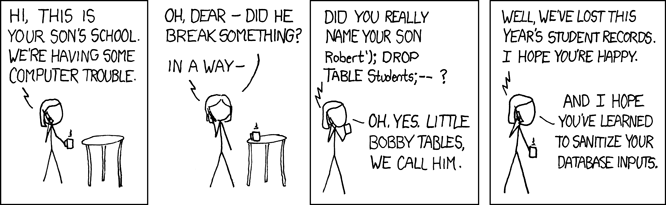
\includegraphics[width=0.95\textwidth]{erros/exploits_of_a_mom.png}
    \fonte{\citeonline{fig_exploits_of_a_mom} / \citeonline{fig_exploits_of_a_mom_explain}.}
    \label{fig:exploits_of_a_mom}
\end{figure}


\section{Erros de modelo de dados}

\begin{itemize}
    \item \erroArmazenarSenhaAberta ;
    
    \item inconsistência na documentação com o método de modelagem utilizado, se a equipe desenvolve a partir de classes utilizando um \ac{orm} que cria as tabelas de forma automática não necessita de um \ac{der}.
    
    \item erro na definição dos modelos apresentados (físico, conceitual, lógico, \ac{der}, \ac{mer}, diagrama de classes);
    
    \item inconsistência entre modelos apresentados (físico, conceitual, lógico, \ac{der}, \ac{mer}, diagrama de classes);

    \item erro na conversão entre modelos;
    
    \item achar que ter um número pequeno de tabelas é mais eficiente que mais tabelas, eficiência tem a ver com modelar corretamente e não com o número de tabelas do banco;
    
    \item dicionário de dados diferente da modelagem apresentada;
    
    \item tipagem de dados incorreta (Ex: um campo para data com tipo VARCHAR);
    
    \item falta de índices adicionais em tabelas do banco de dados, os índices permitem uma busca eficiente sem a leitura completa das tabelas em algumas consultas;
    
    \item falta de teste do modelo definido, muitas vezes não existem campos para armazenamento de informações e também não existem formas de armazenar os dados que se alteram durante o processo e necessitam de histórico;
    
    \item exclusão física de dados que deveriam ser mantidos para histórico;
    
    \item falta de informações para auditoria de processos;
    
    \item erro na escolha de formato de armazenamento de arquivos e imagens (blob ou armazenamento de objetos), cada formato tem vantagens e desvantagens que devem ser considerados de acordo com o contexto da aplicação. Normalmente não faz muito sentido armazenar conteúdos públicos dentro do banco de dados.
    
\end{itemize}

\section{Erros Interface com Usuário}

\begin{itemize}
    \item tradução automática de página via Google tradutor, que acaba gerando falhas de contexto e traduções sem sentido;
    
    \item falta de responsividade em aplicações : web e móvel;
    
    \item não utilizar padrões já existentes para plataforma escolhida;
    
    \item interface complexa para o nível de conhecimento do público alvo da aplicação
    \newline
    \cite{computer_skills}.
    
\end{itemize}

\section{Erros de Validação}

\begin{itemize}
    \item Sistemas de cadastramento que não validam corretamente os dados : falta redigitação de campos importantes como senha;
    
    \item não validar corretamente os campos de acordo com definições existentes (ex e-mail deve seguir \citetitle{rfc5322});
    
    \item falta de validação de e-mail, se o e-mail não for válido o usuário não consegue recuperar a senha (não adianta validar somente o formato, tem que fazer envio com código de validação);
    
    \item falta de sistema seguro para recuperação de senha \cite{forgot_password_cheat_sheet};
    
    \item Limites de senha sem considerar entropia da senha, ex uma senha grande é melhor que uma pequena com diversos tipos de caracteres - \autoref{fig:password_strength};

    \item vulnerabilidade para ataques de injeção - \autoref{fig:exploits_of_a_mom};
    
    \item falta de tratamento no backend, fazendo validações e controle de acesso somente no frontend;
    
\end{itemize}

\begin{figure}
    \centering
    \caption{Boas senhas não devem ser difíceis para o usuário}
	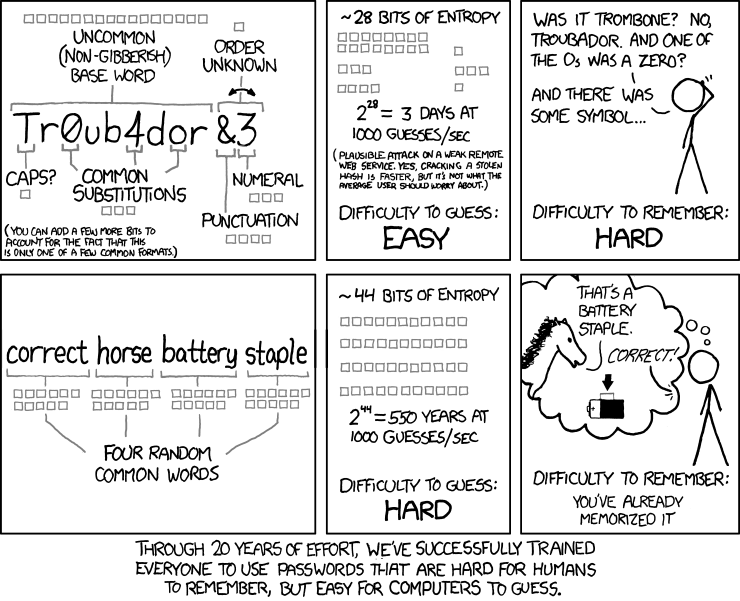
\includegraphics[width=0.95\textwidth]{erros/password_strength.png}
    \fonte{\citeonline{fig_password_strength} / \citeonline{fig_password_strength_explain}.}
    \label{fig:password_strength}
\end{figure}




\section{Erros do processo de teste e apresentação}

\begin{itemize}

    \item testar somente os casos de sucesso sem observar as condições de erro;
    
    \item volume de dados insuficiente para demonstrar o correto funcionamento da aplicação;
    
    \item falta de ordenação nos dados;
    
    \item ordenação sem considerar caracteres de acentuação (ex. Língua deve vir antes de Literatura);
    
% utilizar dados coerentes facilita a apresentação e entendimento da aplicação    
    \item falta de dados consistentes com o contexto da aplicação (escrever teste em um campo pode dificultar posteriormente a analise dos dados).
    
\end{itemize}

\section{Erros de modelagem / análise / projeto}

\begin{itemize}
    \item Casos de uso que não tratam corretamente as ações de usuários, ex recuperação de senha que tem dois passos (solicitar e redefinir senha);
    
    \item definições de casos de uso ou estórias que não detalham claramente o que deve ser feito 
    \newline
    % Instruções exatas como fazer um sanduiche com legendas
    \video{https://www.youtube.com/watch?v=pdhqwbUWf4U}{Como fazer um sanduíche};
    
    \item não analisar corretamente os dados disponíveis para o projeto \cite{boas_perguntas_dados} \cite{guerra-matematica} \cite{ellenberg2015poder} -  \autoref{fig:aviao_wald};
    
    \item desconsiderar o volume de dados e acessos da aplicação ao escolher a arquitetura.
\end{itemize}

\begin{figure}
    \centering
    \caption{Exemplo da análise de \citeonline{wald1980reprint} nos aviões sobreviventes da Segunda Guerra mundial}
	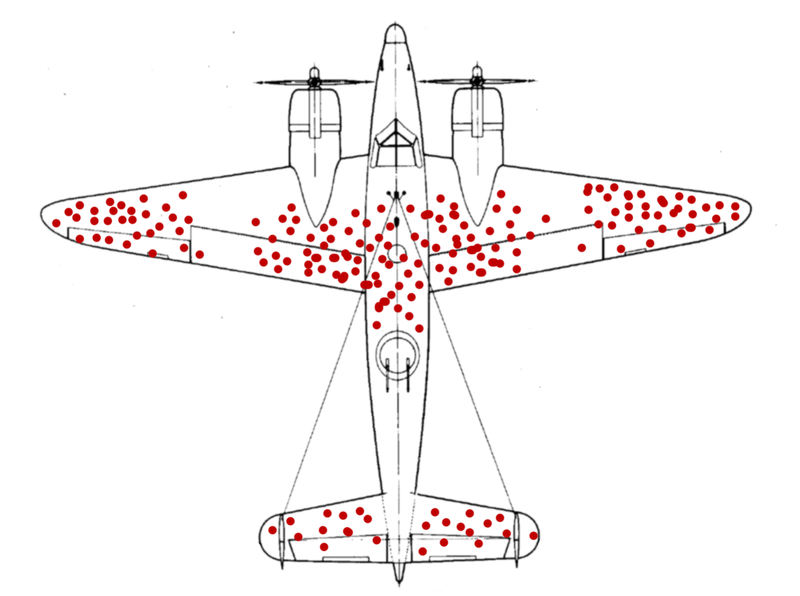
\includegraphics[width=0.8\textwidth]{erros/aviao_wald.png}
    \fonte{\citeonline{fig_aviao_wald}.}
    \label{fig:aviao_wald}
\end{figure}


\section{Erros de planejamento}

\begin{itemize}
    \item Escolher a metodologia X e não utilizar os itens básicos dessa metodologia no desenvolvimento do projeto;
    
    \item escolher \ac{xgh} como metodologia de desenvolvimento \cite{xgh} \cite{xgh-axioms};
    
    \item quem planeja e escolhe a estratégia primeiro tem melhores resultados:
    \begin{itemize}
        \item 
        % Escolha a estratégia correta, corrida sobre tijolos
        \video{https://www.youtube.com/watch?v=4P-i9gCD09s&list=PL69253D27EBEF273E}{Escolha a estratégia correta};
        \item
        % Muito desgate sem planejamento, porquinho buscando cookies sobre geladeira
        \video{https://www.youtube.com/watch?v=LOyX-vgdQGQ&list=PL69253D27EBEF273E}{Muito desgate sem planejamento};
    
        \item % animação : Planejar é Preciso! LEGENDADO
        \video{https://www.youtube.com/watch?v=utLWFdkRm78&list=PL69253D27EBEF273E}{Planejar é Preciso}.    
    \end{itemize}
    
    \item falta de revisão em documentos, aplicação, vídeos;
    
    \item utilizar outras ferramentas e não as obrigatórias das disciplinas, um caso comum é a utilização da ferramenta Postman diretamente (criando a definição manualmente) em vez de utilizar o padrão OpenAPI (swagger) que é obrigatório e que pode ser importado no Postman \cite{postman-openapi};
    
    \item deixar para ultima hora, ex. processos como a criação de documentos no latexdiff, apesar de simples de executar, dependem de preparação de ambiente.
\end{itemize}



\section{Erros de comunicação}

\begin{itemize}
    \item Documentar da melhor maneira para garantir que todos entendam da mesma forma o que deve ser desenvolvido, cuidado com o que escreve:
    \begin{itemize}
        \item \autoref{fig:balanco};
        
        \item \autoref{fig:gabarito-prova};
        
        % Como fazer um sanduiche legendado....
        \item \video{https://www.youtube.com/watch?v=pdhqwbUWf4U&list=PL69253D27EBEF273E}{Como ensinar linguagem de programação para uma criança}.
    \end{itemize}

    \item não acompanhar o e-mail que recebe notificações do \ac{suap}, \gls{moodle};
    
    \item não acompanhar o grupo da disciplina (normalmente no \gls{telegram});
    
    \item falta de comunicação e negociação com os clientes.
\end{itemize}

\todo[inline]{Existem inúmeras versões dessa ilustração \autoref{fig:balanco}, aqui foi utilizada uma publicação como referencia para ilustrar a situação}

\begin{figure}
    \centering
    \caption{A importância da comunicação correta}
	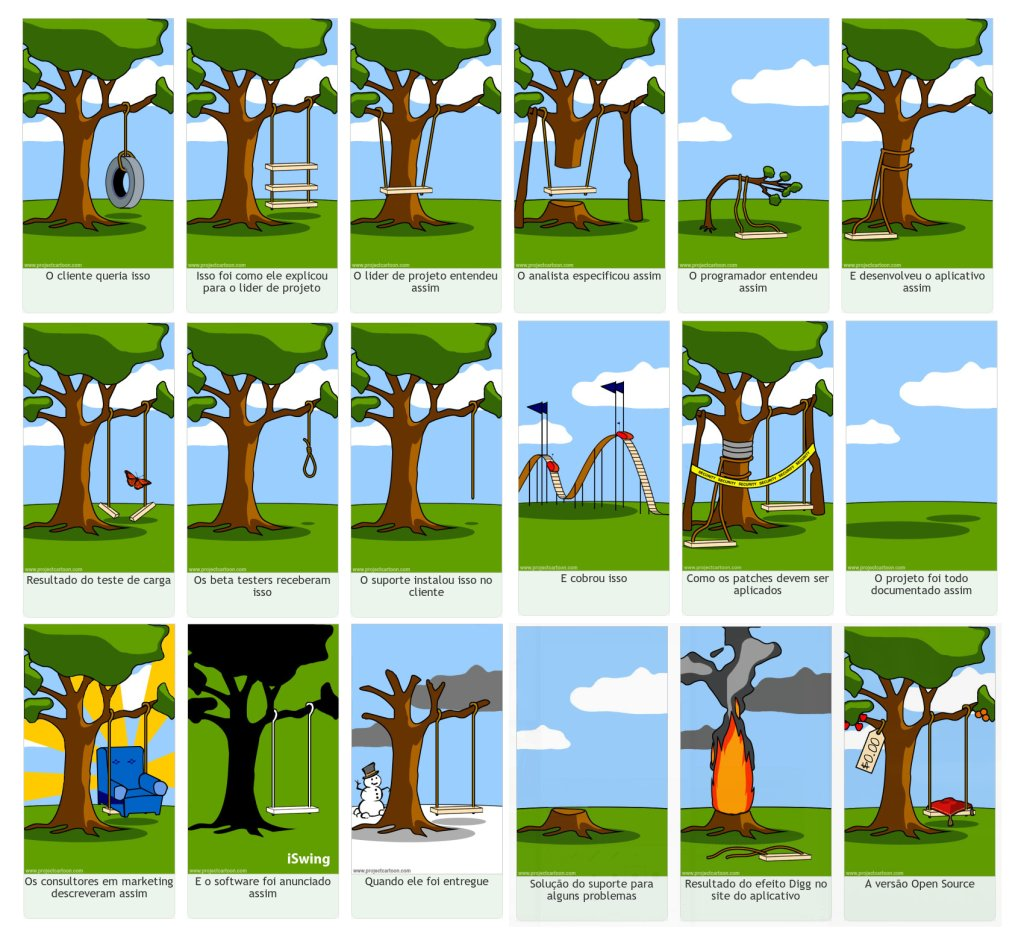
\includegraphics[width=0.95\textwidth]{erros/projeto_balanca_na_arvore.jpg}
    \fonte{\citeonline{engenharia_software_balanca}.}
    \label{fig:balanco}
\end{figure}


\begin{figure}
    \centering
    \caption{A importância da comunicação correta 2}
	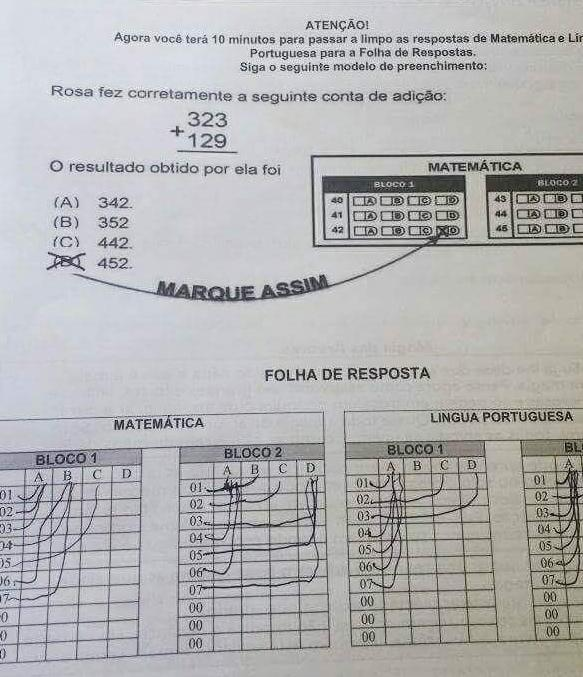
\includegraphics[width=0.95\textwidth]{erros/erro_de_comunicacao_gabarito_prova.jpg}
    \fonte{removida propositalmente.}
    \label{fig:gabarito-prova}
\end{figure}



\section{Erros comportamentais}

Muitos insucessos acontecem devido a comportamentos dos participantes dos projetos, o histórico das disciplinas de projetos demonstraram diversos comportamentos individuais (alguns também acontecem com as equipes) que se evitados permitem melhores resultados:

\begin{itemize}
    \item não escolher os participantes da equipe de acordo com as necessidades do projeto e sim pelas \enquote{amizades} / relações \cite{jackson2019human} \cite{rene_leia_the_human_network} \cite{rene_como_emperrar_a_inovacao};

    \item falta de atenção na leitura dos documentos, regras das disciplinas, mensagens dos professores etc : \autoref{fig:vendo_bolo_cenoura} \cite{atencao_leitura_vendo_bolo_cenoura};
    
    \item medo de errar, para tomar as melhores decisões precisamos de experiencia, e experiencias muitas vezes vem de decisões erradas, mas é importante que essas experiencias aconteçam nos momentos corretos, no inicio e não no final dos projetos \cite{decisions_experience-1} \cite{decisions_experience-2} \autoref{fig:lidar_com_falhas};

    \item não entender o conceito de desenvolvimento de projeto em equipe e responsabilidades: 
    % Diversos videos sobre o trabalho em equipe 
    % Motivacional - Trabalho em equipe - Juntos fazemos mais e melhor!
    \video{https://www.youtube.com/watch?v=twg9SCt76UE&list=PL69253D27EBEF273E}{Trabalho em equipe - Juntos fazemos mais e melhor};
    
    \item não buscar as informações originais que normalmente se encontram em língua inglesa. Muitos documentos da área foram escritos em inglês e possuem traduções com erros técnicos, por isso é importante buscar os documentos originais e não utilizar traduções de terceiros;
    
    \item falta de foco: 
    % A importância de manter o foco!
    % Urso na fila de atendimento....
    \video{https://www.youtube.com/watch?v=6SRTQbBjrFs&list=PL69253D27EBEF273E}{A importância de manter o foco!};
    
    \item focar na tarefa e não no resultado:
    % fazendo trico / cachecol
    \video{https://www.youtube.com/watch?v=J0iv3TqJBV8&list=PL69253D27EBEF273E}{Foco na Tarefa x Foco no Resultado};
    
    \item falta de comprometimento: 
    \autoref{fig:scrum} e 
    \citeonline{meligeni_primeiro_treino};

    \item não acreditar no seu potencial: 
    % Desafio de Gigantes - carregando outro nas costas pelo campo todo...
    \video{https://www.youtube.com/watch?v=7UnyWuu8HK0&list=PL69253D27EBEF273E}{Trecho do filme Desafiando Gigantes - 2006}
    e
    % Rocky Balboa - Motivação Sensacional
    % Outras versões : 
    % https://www.youtube.com/watch?v=JeLYCrE5MrI
    % https://www.youtube.com/watch?v=Rhr6qO7Gmu0
    \video{https://www.youtube.com/watch?v=Qxsyy5H9JTk&list=PL69253D27EBEF273E}{Trecho do filme Rocky Balboa - 2006};
    
    \item medo de sair da zona de conforto:
    % Até a lagosta sente o desconforto do crescimento
    \video{https://www.youtube.com/watch?v=F8VBA89qWpc&list=PL69253D27EBEF273E}{Até a lagosta sente o desconforto do crescimento};
    
    \item falta de motivação, não encarar os desafios, pode ser falta de um \enquote{tubarão} \cite{tubarao_na_vida} \cite{put_a_shark_in_your_tank} \cite{employees_challenge};
    
    \item erro no gerenciamento do tempo e atividades:
    \begin{itemize}
        \item \enquote{macacos no ombro}:
    \waUrl{https://prazercompartilharblog.wordpress.com/2017/09/15/tire-os-macacos-do-meu-ombro/}
    e
    % TIRE O MACACO DO OMBRO
    \video{https://www.youtube.com/watch?v=7alQeDOtiRQ&list=PL69253D27EBEF273E}{TIRE O MACACO DO OMBRO});
    
        \item \video{https://www.youtube.com/watch?v=arj7oStGLkU}{Inside the mind of a master procrastinator} \cite{ted_tim_urban_procastinator}.
    \end{itemize}

    \item deixar para ultima hora o estudo das atividades (latexdiff, statsvn, gource entre outras são ferramentas simples, mas dependem de preparação do ambiente para serem utilizadas);

    \item Não utilizar o conhecimento da equipe para resolver os problemas e fazer as escolhas - \autoref{fig:conhecimento_h2o};
    
    \item Não utilizar os recursos e ferramentas existentes da forma correta - \autoref{fig:uso_recursos_escada_1} e \autoref{fig:uso_recursos_escada_2};

\todo[inline]{Migrar links para referencias e utilizar opções do biblatex}
    \item Não aproveitar os aprendizados de outros alunos que já passaram pelas disciplinas de projetos :
    \begin{itemize}
        \item \waUrlTitle{https://glybif.blogspot.com.br/2016/12/como-ir-bem-em-pds.html}{Como ir bem em PDS? - GLYBIF - 2016};

        \item \waUrlTitle{https://glybif.blogspot.com/2020/04/4-anos-depois-de-fazer-pds.html}{4 anos depois de fazer PDS - GLYBIF - 2020};

        \item \waUrlTitle{https://projetothewalkingpet.blogspot.com/2018/12/dificuldades-e-licoes-aprendidas.html}{Dificuldades e lições aprendidas - The WalkingPet - 2018};

        \item \waUrlTitle{https://projetoa6pgpgrupo101010.blogspot.com/2018/12/o-que-nao-fazer-em-a6pgp-para-que-sofrer.html}{O que NÃO fazer em A6PGP: Para quê sofrer? - Blood 4 Pets - 2018};
        
        \item \waUrlTitle{https://projetoa6pgpgrupo101010.blogspot.com/2018/12/licoes-aprendidas-durante-o-semestre.html}{Lições aprendidas durante o semestre - Blood 4 Pets - 2018};

        \item \waUrlTitle{https://pgppain.blogspot.com/2019/03/19-coisas-que-voce-precisa-saber-sobre.html}{19 coisas que você precisa saber sobre a Prova de Conceito - PGPPain - 2019};

        \item \waUrlTitle{https://pgppain.blogspot.com/2019/03/nos-estamos-atrasados.html}{Nós estamos atrasados - PGPPain - 2019};

        \item \waUrlTitle{https://ginquestapp.wordpress.com/category/dicas-de-sobrevivencia/}{Dicas de Sobrevivência - GinQuest - 2019}.

    \end{itemize}
    
    \item falta de cuidado na comunicação dentro da equipe para garantir o objetivo.
    
\end{itemize}

\begin{figure}
    \centering
    \caption{Erro na interpretação das mensagens ou falta de atenção}
	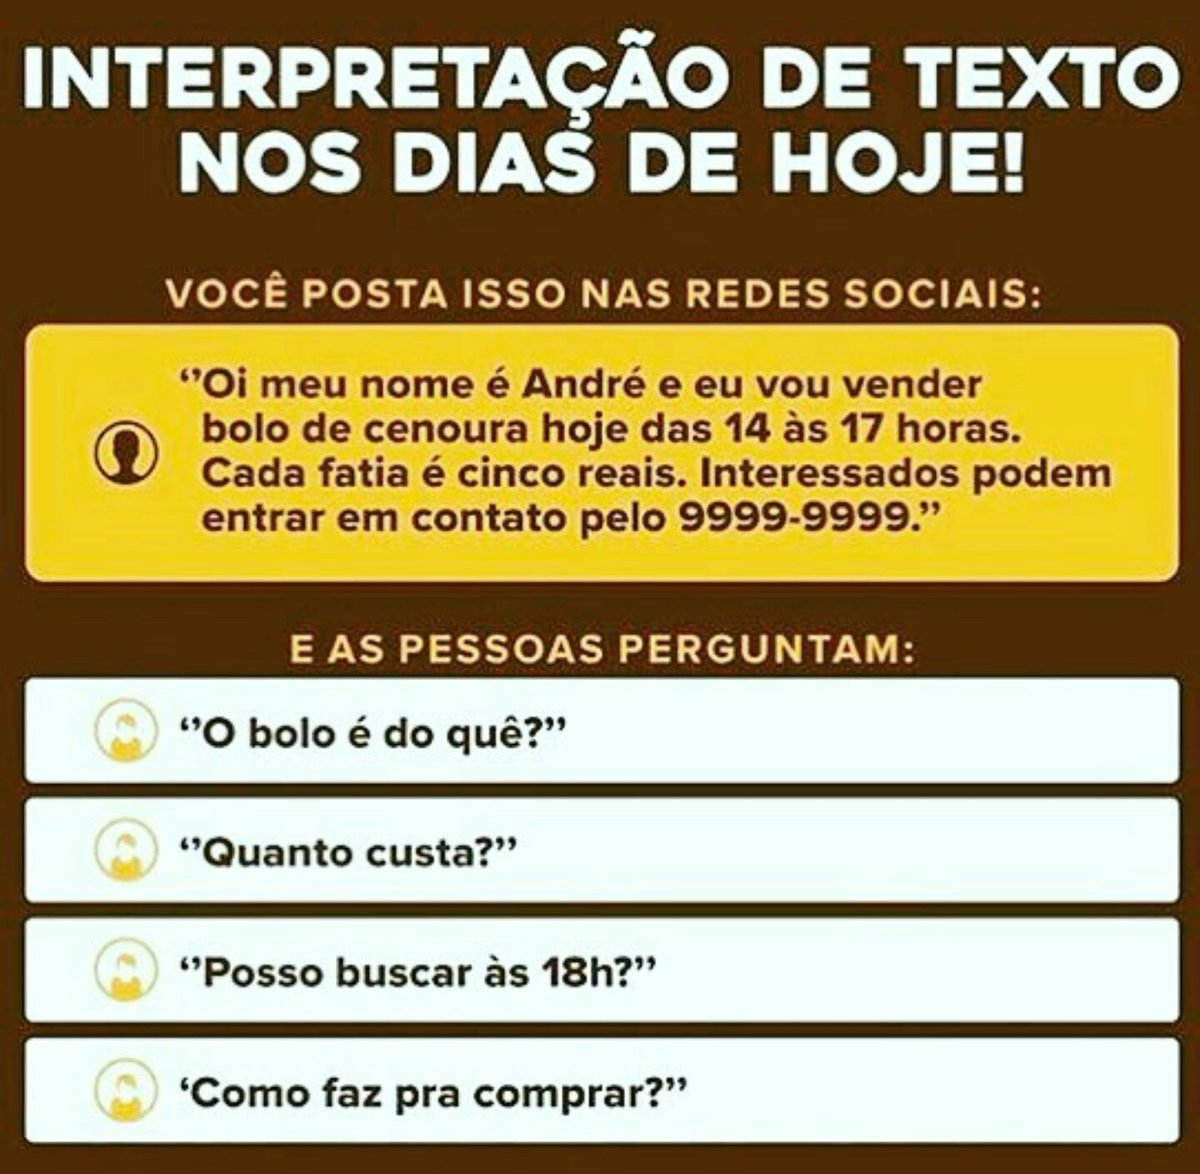
\includegraphics[width=0.95\textwidth]{erros/vendo_bolo_cenoura.jpg}
	\fonte{Autor desconhecido.}
    \label{fig:vendo_bolo_cenoura}
\end{figure}



\begin{figure}
    \centering
    \caption{Comprometimento}
	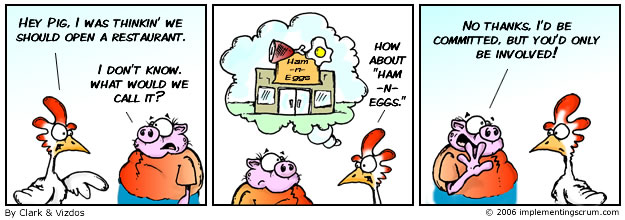
\includegraphics[width=0.95\textwidth]{erros/060911-scrumtoon.jpg}
    \fonte{\citeonline{scrum_cartoon}.}
    \label{fig:scrum}
\end{figure}

\begin{figure}
    \centering
    \caption{Utilizar o conhecimento}
	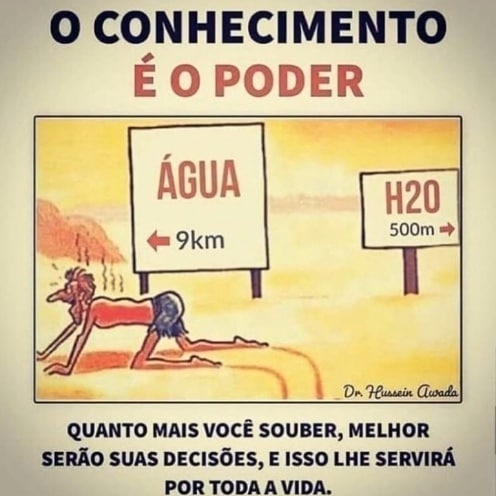
\includegraphics[width=0.7\textwidth]{erros/conhecimento_h2o.jpg}
    \fonte{Hussein Awada, -.}
    \label{fig:conhecimento_h2o}
\end{figure}

\begin{figure}
    \centering
    \caption{Saiba utilizar corretamente seus recursos}
	
\includegraphics[width=0.7\textwidth]{erros/uso_de_recursos_escada_1.jpg}
    \fonte{\citeonline{paulo_maciel_utilizar_recursos}.}
    \label{fig:uso_recursos_escada_1}
\end{figure}

\begin{figure}
    \centering
    \caption{Saiba utilizar corretamente seus recursos - Comparação}
	
\includegraphics[width=0.7\textwidth]{erros/uso_de_recursos_escada_2.jpg}
    \fonte{\citeonline{paulo_maciel_utilizar_recursos_comparado}.}
    \label{fig:uso_recursos_escada_2}
\end{figure}




\begin{figure}
    \centering
    \caption{Aprenda a lidar com suas falhas}
	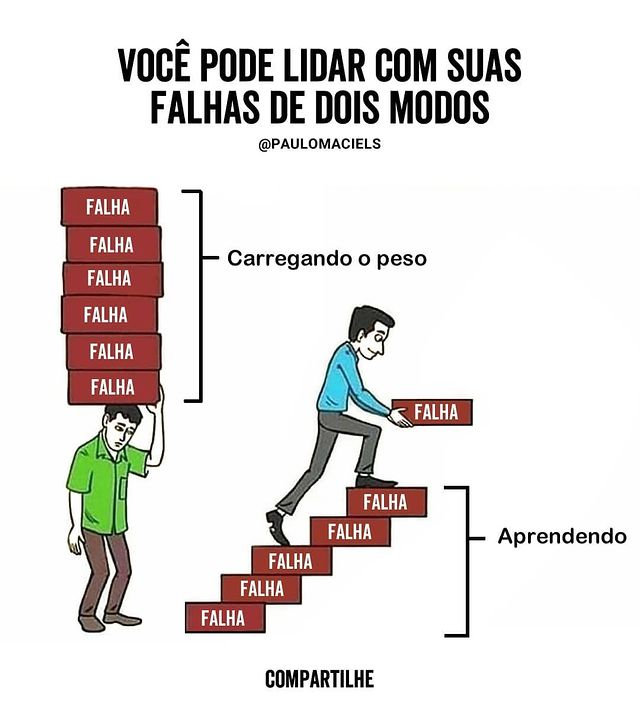
\includegraphics[width=0.7\textwidth]{erros/lidar_com_falhas.jpg}
    \fonte{\citeonline{paulo_maciel_lidar_com_falhas}.}
    \label{fig:lidar_com_falhas}
\end{figure}


%\chapter{Revisão de Textos e apresentações}
\label{revisao-de-textos}

\todo[inline]{fazer as ligações com as seções de erros}

A revisão do documento e da apresentação antes da entrega evita que os erros sejam apresentados no resultado final. Esse capítulo indica alguns procedimentos que evitam esse tipo de ocorrência. É importante lembrar que alguns elementos apresentados nos capítulos anteriores como erros também devem ser verificados para garantir a qualidade do seu trabalho.

\begin{itemize}
    \item Passar corretor ortográfico no documento (o ideal é já utilizar um editor que faça a verificação durante a edição e ir corrigindo durante a edição);

    \item Faça a revisão em cima da versão final em \ac{pdf} com a formatação final;
    
    \item Utilize uma ferramenta de online de anotações no \ac{pdf} \url{https://dicas.ivanfm.com/aulas/textos/anotacoes-em-documentos.html} para facilitar o controle de anotações e histórico disponível para todos de forma online e centralizada;
    
    \item Faça uma leitura em voz alta, isso reduz a sua velocidade de leitura e aumenta a concentração, facilitando a percepção dos erros no texto;
    
    \item Solicite a diversas pessoas que participem da revisão, mesmo as pessoas que não entendem a parte técnica podem ajudar na revisão do texto;
    
    \item Coloque a data no nome do arquivo para facilitar a organização das versões compartilhadas;
    
    \item Para documentos gerados com \LaTeX, limpe todos os temporários / caches e compile do zero para garantir que todos os índices sejam atualizados;
    
    \item Verifique se a numeração das páginas é compatível com o formato de impressão (Frente/Verso ou somente Frente);
    
    \item Caso tenha páginas em A3 e impressão Frente/Verso cuidado para não alterar a posição das páginas na mudança;
    
    \item Verificar lista de siglas, siglas em outras línguas devem ter a tradução para português;

    \item Verificar listas de figuras, quadros e tabelas - \autoref{revisao-listas};

    \item fazer buscas no documento para encontrar os erros mais comuns - \autoref{buscas-documento};
    
    \item Listas de itens devem ser separados ponto e virgula nos itens iniciais e ponto no último item;
    
    \item Listas de itens devem seguir uma ordem coerente (lógica ou alfabética) e não aleatória (por exemplo essa lista segue uma sequencia que considera uma ordem a ser seguida para executar a revisão);
    
    \item Não devem existir espaços em branco no meio dos capítulos, não forçar quebras manualmente;
    
    \item verificar os tempos verbais (a leitura do documento acontece depois do desenvolvimento);
    
    \item Todos itens (capítulos, seções, subseções) devem possuir texto ( ideal que tenha pelo menos três parágrafos ) - ver \autoref{erros-comuns-sub1};

    \item Verificar palavras de outras línguas - ver \autoref{revisao-palavras-estrangeiras};
    
    \item Padronização de nomenclatura : o é \textbf{XYZ} ou \textbf{Xyz} utilizar um único formato em todos locais.
    
\end{itemize}

\section{Verificação das listas de elementos do documento}
\label{revisao-listas}

As listas de ilustrações (figuras, quadros, tabelas etc) e o sumário devem ser verificadas com cuidado :

\begin{itemize}
    \item não devem conter elementos com mesmo titulo, cada elemento deve ter um titulo único;
    
    \item caso existam vários elementos parecidos verifique se o formato de nomes segue um mesmo padrão.
    \todo[inline]{vale criar um exemplo na seção de erros}
    
\end{itemize}

\section{Buscas que podem encontrar problemas no documento}
\label{buscas-documento}

\begin{itemize}
    \item \textbf{??} para encontrar referências quebradas, já que o \LaTeX \space indica com \textbf{??} quando não encontra uma referencia;
    
    \item Buscar por \textbf{Figura}, \textbf{Quadro}, \textbf{Tabela} etc
    
        \begin{itemize}
            \item verificar se os artigos ( feminino / masculino ,  a / o  ) estão corretos;
           
            \item Verificar se tabelas e quadros foram definidos corretamente, repeitando os formatos de cada tipo;
            
            \item verificar se o tipo e o número da ilustração estão como link (autoref);
           
            \item Colunas com valores numéricos em tabelas / quadros devem ser alinhadas à direita;
           
            \item Verificar se toda ilustração foi citada no texto;
           
            \item Verificar se gráfico colorido vai ficar legível na impressão preto e branco;
            
            \item Verificar se as citações e referencias estão como links (no caso do \LaTeX \space utilizando esse modelo ficam em cor azul);
          
            \item Verifique se as referencias do texto para as ilustrações estão na sequencia correta (a \textbf{figura n} deve ser referenciada antes da \textbf{figura n+x}).  
        \end{itemize}
        
    \item Buscar por cada elemento da lista de siglas / abreviações- ver \autoref{buscas-siglas};
    
    \item Buscar por cada elemento do glossário - ver \autoref{buscas-glossario};
            
    \item Buscar por \textbf{"} (aspas), verificar se não está grudada no texto anterior / seguinte;
    
    \item Buscar por \textbf{(} e \textbf{)} (parênteses) para verificar citações - ver \autoref{erros-citacoes-indiretas}
        \begin{itemize}
            \item Verificar se o formato da citação é compatível com o texto / local onde se encontram;
            
            \item Verificar se citações não ficaram grudadas no texto.
        \end{itemize}
            
    \item Buscar por \textbf{[S.l.]} e \textbf{[S.n.]}, vai encontrar referencias incompletas de livros.
\end{itemize}

\section{Revisão de siglas}
\label{buscas-siglas}

As siglas (ex \ac{ifsp}) devem seguir um padrão dentro do documento, buscar por cada elemento na lista de siglas permite determinar se foram definidas corretamente :

\begin{itemize}
    \item Primeira ocorrência deve ter nome por extenso;
    
    \item Primeira ocorrência por extenso não deve aparecer nas listas (figuras, tabelas etc), ao verificar a lista de siglas se o número de página de utilização de sigla for anterior ao da lista de siglas precisa ajustar para utilizar \mostraComandoLaTeX{acs} no título da ilustração;

    \item No documento gerado com \LaTeX \space todas utilizações devem ser links.
\end{itemize}

Mas se durante a leitura do documento encontrar alguma sigla que não esteja indicada com o link essa sigla não foi definida corretamente dentro do documento \LaTeX  \space como uma sigla.

\section{Revisão de glossário}
\label{buscas-glossario}

Como o \LaTeX \space faz a referencia de glossário como um link é importante buscar no documento pelas palavras do glossário e verificar se estão com o link. Também é importante solicitar que os revisores que não fazem parte da escrita do documento anotem os termos que tem dúvidas já que isso é um bom indicador de palavras que devem ser incluídas no glossário.


\section{Revisão de Palavras de outras Línguas}
\label{revisao-palavras-estrangeiras}

De acordo com a \ac{abnt} as palavras estrangeiras devem ser utilizadas com itálico (exceto nomes próprios), mas também deve ser tomado o cuidado já que muitas vezes precisamos incluir um artigo juntamente com a palavra, portanto é necessário verificar  se está utilizando artigo de forma correta :

\begin{itemize}
    \item \textbf{o \textit{sprint}} ou \textbf{a \textit{sprint}} são validos mas deve ser utilizado de forma uniforme em todo o texto e de acordo com a definição utilizada 
    \begin{itemize}
        \item se \textit{sprint} for definido como um período de tempo, ciclo de desenvolvimento deve utilizar o artigo \textbf{o};
        
        \item se a definição é como uma etapa ou fase de desenvolvimento deve utilizar o artigo \textbf{a}.
    \end{itemize}
    
\end{itemize}


\section{Revisão de Apresentações}
\label{revisao-apresentacoes}

Em apresentações alguns detalhes adicionais devem ser considerados como contraste entre os elementos utilizados e se cores forem utilizadas para demonstrar alguma informação se todos podem ver essa informação (considerando que algumas pessoas não conseguem visualizar todas as cores é sempre bom utilizar ícones na representação. Se a apresentação for feita com o uso de um projetor é importante testar antecipadamente para garantir que o projetor consiga apresentar corretamente as cores e resolução utilizadas.







% ---
% Conclusão (outro exemplo de capítulo sem numeração e presente no sumário)
% Dependendo do trabalho desenvolvido ele pode ter uma Conclusão ou Considerações finais
% Para trabalhos de disciplina utilizar Considerações Finais
% ---
\chapter{Considerações Finais}

Esse capítulo tem como intuito descrever o desenvolvimento da aplicação feita pela equipe, demonstrando as dificuldades no decorrer do projeto. Como também informando as lições aprendidas com essa experiência.

\section{Principais Dificuldades}
Desde o início do projeto, foi compreendido pelos componentes que não seria um trabalho fácil, seria necessário auto-disciplina, dedicação  e principalmente, o apoio coletivo da equipe. De maneira inicial, foi difícil, visto que a equipe encontrava-se em níveis diferentes de conhecimento e desenvolvimento. \\
 No início, a dificuldade encontrada, ocorreu quando os integrantes da equipe tinham tempo limitado para o desenvolvimento do projeto. Os integrantes trabalham em tempo integral, fazendo com que, o único tempo disponível seria de noite ou finais de semana. Mesmo reorganizando as funções, cada integrante não teria muito tempo para realizar as funções destinadas a cada um. \\
Imprevistos aconteceram durante a semana, onde interferiu diretamente no projeto. Desse jeito, dois integrantes do grupo saíram, o Kelvin e o Lucas, aumentando a carga de trabalho e a responsabilidade de todos.\\
A segunda dificuldade ocorreu quando os integrantes informaram que teriam conhecimentos básicos com as tecnologias utilizadas, como React Native, PostgreSQL, Expo, etc. Nem todos possuíam uma grande curva de aprendizado e, devido a pouca disponibilidade, isso acabou atrapalhando o desenvolvimento do projeto. Como tentativa de amenizar esse problema, realizamos algumas videochamadas para nos ajudarmos.\\


\section{Lições Aprendidas}
Ao decorrer do projeto, a equipe observou que teria que se comunicar melhor sobre o projeto, para evitar retrabalhos, pois com a falta dessa comunicação fez com que alguns tópicos fossem refeitos como, os Casos de Uso, MER, DER, etc.\\
Os Wireframes passaram a ser refeitos no decorrer do projeto, por conta das correções de funcionalidades do usuário. \\
Após identificar os pontos de melhoria, as mudanças nos padrões de comportamento trouxeram muito mais união à equipe. Observaram-se muitos pontos positivos durante o desenvolvimento, relacionados à empatia, paciência  e esforço de cada integrante durante o trabalho. Desta forma, a equipe teve uma melhora muito grande ao final do projeto. \\


\section{Funcionalidades Futuras}
Por se tratar de um aplicativo de transporte, o projeto tem potencial para ter grandes mudanças no decorrer do tempo e das necessidades que vão aparecer, de melhoria e atualizações que podem abranger leis e normas públicas, como novas funcionalidades para usuários, de modo que o App se torne mais atrativo para os usuário e futuras parcerias. Por exemplo, a inclusão de transporte de Pets usando aviões em viagens nacionais como internacionais.\\
Para o futuro, buscamos ter grande aproveitamento no crescimento do aplicativo para uso não só em território nacional como internacional, gerando assim questões como mais idiomas para o aplicativo, usar servidores externos ou até mesmo parcerias fora do Brasil.\\
Visando o cliente final, é desejado ter uma interface mais simples visando pessoas idosas ou que não possuem grande conhecimento em tecnologia usando aplicativos.\\





% ----------------------------------------------------------
% Glossário
% ----------------------------------------------------------
%
%
\ifdef{\printnoidxglossary}{
    \addcontentsline{toc}{chapter}{GLOSSÁRIO}
    \printnoidxglossary[style=glossario]
    %\printglossaries
}{}
\chapter{Referências}
ABINPET. Mercado Pet Brasil 2021. Disponível em: <http://www.abinpet.org.br/download/abinpet_folder_2021.pdf> Acesso em 14 de Abril de 2022.
INSTITUTO PET BRASIL.Censo Pet: 139,3 milhões de animais de estimação no Brasil.2019.Disponível em: <http://institutopetbrasil.com/imprensa/censo-pet-1393-milhoes-de-animais-de-estimacao-no-brasil/> Acesso em: 14 de Abril de 2022.
GOVERNO FEDERAL DO BRASIL. O Brasil registrou mais de 234 milhões de acessos móveis em 2020. Agência Nacional de Telecomunicações. 2021. Disponível em: <https://www.gov.br/pt-br/noticias/transito-e-transportes/2021/05/brasil-registrou-mais-de-234-milhoes-de-acessos-moveis-em-2020> Acesso em: 14 de Abril de 2022.
HEROKU. Heroku Pricing. 2020. Disponível em: <https://www.heroku.com/pricing#app-types-header>.Acesso em: 14 abr. 2022.
RIBEIRO, A. F. de A. Cães Domesticados e os benefícios da interação. Revista Brasileira de Direito Animal, Salvador, v. 6, n. 8, 2014. DOI: 10.9771/rbda.v6i8.11062. Disponível em: https://periodicos.ufba.br/index.php/RBDA/article/view/11062. Acesso em: 14 abr. 2022.
SILVA, N. A.; MARISCO, G. A RELAÇÃO DE ANIMAIS DOMÉSTICOS NA EDUCAÇÃO E SAÚDE. Interfaces Científicas - Saúde e Ambiente, [S. l.], v. 7, n. 1, p. 71–78, 2018. DOI: 10.17564/2316-3798.2018v7n1p71-78. Disponível em: https://periodicos.set.edu.br/saude/article/view/5491. Acesso em: 14 abr. 2022.
SOUZA, A. S. de. Direitos dos animais domésticos: análise comparativa dos estatutos de proteção. Revista de Direito Econômico e Socioambiental. v. 5, n. 1, p. 110–132, 2014. Disponível em: <https://periodicos.pucpr.br/direitoeconomico/article/view/6242>. Acesso em: 14 abr. 2022.
GOOGLE PLAY CONSOLE. Disponível em: <https://play.google.com/console/u/0/signup>.Acesso em: 16 abr. 2022.
APPLE DEVELOPER PROGRAM.Isenção da taxa de assinatura no Apple Developer Program
. Disponível em: <https://play.google.com/console/u/0/signup>.Acesso em: 16 abr. 2022.
Docker. Docker Pricing. 2022. Disponível em: <https://www.docker.com/pricing/>.Acesso em: 16 abr. 2022.
GREGOL, R. E. W. Recursos de escalabilidade e alta disponibilidade para aplicações web.Repositório de Outras Coleções Abertas, p. 17–18, 2011.
ENDEAVOR. Quão longe sua ideia pode ir? Descubra avaliando a escalabilidade dela. 2015. Disponível em: <https://endeavor.org.br/estrategia-e-gestao/escalabilidade/>.Acesso em: 17 abr. 2022.
GOOGLE DEVELOPERS. Disponível em: <https://developer.android.com/docs/quality-guidelines/core-app-quality?hl=pt-br#sc>.Acesso em: 18 abr. 2022.
BRASIL. Lei Geral de Proteção de Dados (2018). 2018. Disponível em: <http://web.archive.org/web/20200915225322/http://www.planalto.gov.br/ccivil_03/_ato2015-2018/2018/lei/L13709.htm>. Acesso em: 18 abr. 2022.
 MARTIN FOWLER.Continuous Integration. 2001.Disponível em: <https://martinfowler.com/articles/continuousIntegration.html>.Acesso em: 18 abr. 2022.
PESSANHA, L.; PORTILHO, F. Comportamentos e padrões de consumo familiar em torno dos “pets”. IV ENEC - Encontro Nacional de Estudos do Consumo, 2008.
GRAF, C. T. O comportamento do consumidor no mercado pet e a relação entre os cães e as pessoas. Universidade Regional do Noroeste do Estado do Rio Grande do Sul, 2016.
CHEN, A.; HUNG, K.; PENG, N. A cluster analysis examination of pet owners ’consumption values and behavior –segmenting owners strategically. Journal of Targeting, Measurement and Analysis for Marketing, v. 20, n. 2, p. 117–132, 2012.
Silvaet.al.Petshow.2021.Disponível em:<https://svn.spo.ifsp.edu.br/svn/a6pgp/S202001-PI/HYVE/Documentos/5-EntregaFina>.Acesso em: 01 mai. 2022.
PRODEST.O uso de aplicativos na sociedade.Disponível em:
<https://prodest.es.gov.br/o-uso-de-aplicativos-na-sociedade#:~:text=Os\%20aplicativos\%20fazem\%20cada\%20vez,op\%C3\%A7\%C3\%B5es\%20de\%20lazer\%20com\%20facilidade.> Acesso em: 03 mai. 2022.
CARVALHO, J. O. F. D. O papel da interação humano-computador na inclusão digital. Transformação, V. 15, n. spe, p. 75-89. Campinas, Dezembro, 2003 .Disponível em: <http://www.scielo.br/scielo.php?script=sci_arttext&pid=S0103-37862003000500004&lng=en&nrm=iso>. Acesso em: 03 mai. 2022.
GLOBOESPORTE.COM. Uso de aplicativos de saúde deve aumentar nos
próximos anos, segundo pesquisa. Grupo Globo. Rio de Janeiro.2019. Disponível
em:<https://globoesporte.globo.com/eu-atleta/noticia/uso-de-aplicativos-de-saude-deve-aumentar-nos-proximos-anos-segundo-pesquisa.ghtml> .  Acesso em: 03 mai. 2022
BRITO, S. Quem usa mais o smartphone: Brasil ou Estados Unidos? Revista Veja digital. Editora Abril. Janeiro de 2021. Disponível em: 
<https://veja.abril.com.br/tecnologia/quem-usa-mais-o-smartphone-brasil-ou-estados-unidos/> . Acesso em: 03 mai. 2022.
SANTOS, A. Brasil, segundo país onde o mercado de aplicativos mais cresce.Terra.2020. Disponível em:<https://www.terra.com.br/noticias/dino/brasil-segundo-pais-onde-o-mercado-de-aplicativos-mais-cresce,1fd9d38aa995ad8ca1243f6c58080f79u2ee8tfj.html#:~:text=Os\%\%20realizados\%20pela\%20empresa,m\%C3\%A9dio\%20real\%20de\%2030\%20apps.&text=Houve\%20um\%20aumento\%20de\%2030,aplicativos\%20do\%20Google\%2C\%20em\%202020> .  Acesso em: 03 mai. 2022.
INSTITUTO PET BRASIL. Censo Pet: 139,3 milhões de animais de estimação no Brasil. 2019. Disponível em: <http://institutopetbrasil.com/imprensa/censo-pet-1393-milhoes-de-animais-de-estimacao-no-brasil/>. Acesso em: 19 mai. 2022.
PUGA, E. F. e. M. G. S. Banco de dados: Implementação em SQL, PL/SQL e Oracle 11g. 1. ed. São Paulo: Pearson Universidades, 2013. Acesso em: 21 mai. 2022.
IBM. Arquitetura de três camadas. 2020. Disponível em: 
<https://www.ibm.com/br-pt/cloud/learn/three-tier-architecture#toc-benefcios--jxGrdA7u>. Acesso em: 22 mai. 2022.
https://www.w3schools.com/js/js_conventions.asp

% ----------------------------------------------------------
% Apêndices
% Documentos gerados pelo próprio autor
% ----------------------------------------------------------

% ---
% Inicia os apêndices
% ---
\begin{apendicesenv}

% Imprime uma página indicando o início dos apêndices
\partapendices

% ----------------------------------------------------------
\chapter{QUESTÃO DE PESQUISA}
% ----------------------------------------------------------

\subsection{Como os animais são transportados ?}
\label{p1}
\subsection{Como solicitar uma viagem ?}
\label{p2}
\subsection{Como será a higienização do carro?}
\label{p3}
\subsection{O aplicativo irá permitir quantos animais no carro ?}
\label{p4}
\subsection{O aplicativo terá agendamentos ?}
\label{p5}
\subsection{Será possível, que o animal viaje sem o seu dono ?}
\label{p6}
\subsection{Teremos parcerias ?}
\label{p7}
\subsection{Como serão os métodos de pagamentos e como esse valor será cobrado ?}
\label{p8}
\subsection{Como será a comunicação entre o passageiro e o motorista ?}
\label{p9}
\subsection{Como será o método de contratação do motorista ?}
\label{p10}
\subsection{Como será o método de avaliação do motorista ?}
\label{p11}
\subsection{Como será o benefício comum e o premium ?}
\label{p12}
\subsection{Como será o histórico de corridas ?}
\label{p13}
\subsection{Quais animais serão permitidos ?}
\label{p14}
\subsection{Será cobrado alguma taxa extra aos passageiros, para os condutores conseguirem realizar a manutenção no carro a cada viagem ?}
\label{p15}
\subsection{Como será definida a rota de transporte ?}
\label{p16}
\subsection{Como será o chat durante a corrida ?}
\label{p17}
\subsection{Como funcionará o sistema de pontos fidelidade ?}
\label{p18}
\subsection{Como vai funcionar a compra de descontos (Sistemas de pontos)  ?}\label{p19}

\section{Respostas }\\
\subsection{Resposta da pergunta \ref{p1}}
No Carrara Pets, para garantir a segurança e o conforto aos animais, cães usam um cinto de segurança especial que prende no gancho da coleira, e os gatos são transportados dentro de uma caixa específica. Os veículos são higienizados ao final de cada viagem. Caso o pet realize a viagem sozinho, a plataforma envia um SMS automático ao usuário que a corrida foi finalizada, mas também é possível acompanhar o percurso em tempo real por meio do aplicativo. Com o aplicativo, é possível acompanhar a viagem em tempo real, e o pagamento é feito pelo aplicativo.

\subsection{Resposta da pergunta \ref{p2}}
Para solicitar uma corrida, basta abrir o aplicativo e informar os locais de encontro e de destino. O usuário pode acompanhar o trajeto em tempo real, e também consegue realizar o agendamento de corridas. O pagamento pode ser feito com cartão de crédito, a um preço fixo. Com o objetivo de garantir um bom atendimento, é possível visualizar a avaliação dos motoristas, feita por outros usuários da plataforma.

\subsection{Resposta da pergunta \ref{p3}}
Todos os veículos estarão equipados com Kit de proteção que inclui guia, cinto peitoral e focinheira para cães. No caso dos gatos, conectamos a sua caixa de transporte própria ao nosso sistema de segurança. A higiene do veículo também é bastante cuidadosa. Os bancos possuem uma capa protetora de assento, que são aspiradas ao final de cada corrida e recebem uma solução fungicida (combate fungos), viricida (inibe a proliferação de um vírus num processo infeccioso) e bactericida (antibióticos que destroem bactérias) de uso veterinário. É um processo muito importante, pois evita disseminação de doenças entre os animais e humanos também, além de deixar o carro limpo para a próxima corrida.

\subsection{Resposta da pergunta \ref{p4}}
No aplicativo iremos possuir um campo específico para informar a quantidade de pets que irão viajar no veículo e os portes dos animais. 
\textbf{Regras:} 
\begin{itemize}
    \item 1 animal - porte grande, médio ou pequeno.
    \item 2 animais - porte grande e um médio 
    \item 3 animais - porte médio e pequeno 
    \item 4 animais - porte pequeno.
\end{itemize} 

\subsection{Resposta da pergunta \ref{p5}}
Sim. Você contará com a comodidade de agendamento prévio de corridas. Funciona do seguinte modo: você seleciona o dia, a hora e o local para o nosso motorista ir buscar o seu pet e você no local solicitado.

\subsection{Resposta da pergunta \ref{p6}}
Sim. Você poderá realizar o despacho do seu pet desacompanhado. Você não vai precisar acompanhá-lo na viagem se não puder ou quiser, basta ter um responsável para entregar o animal ao motorista no local de origem e outro para receber no local de destino. 
\textit{Pontos Negativos com o serviço de transportes de passageiros ou públicos para deslocar com o seu pet:}
\begin{enumerate}
    \item Insegurança - a falta de equipamentos de segurança para prender corretamente o seu pet ao cinto de segurança e a falta de conhecimento do condutos podem causar acidentes.
    \item Desrespeito às normas de trânsito - O código de trânsito brasileiro (CTB) estabelece normas para o transporte dos animais, motoristas que não possuem treinamentos específicos, podem desconhecê-las e acabam transportando o seu cão de forma errada. 
    \item Motorista despreparados - o motorista não tem experiência e nem treinamento para fazer o transporte dos pet. Além disso, podem ficar irritados se o animal fizer sujeira no carro. 
    \item Falta de equipamentos - os veículos comuns não possuem os acessórios de segurança e higiene para pet.
\end{enumerate}

\subsection{Resposta da pergunta \ref{p7}}
Sim. Iremos ter parcerias com estabelecimentos de pet, como Pet Shop, veterinário, Banho e Tosa. Caso a pessoa seja dono ou gestor de um estabelecimento, poderá entrar em contato conosco e pedir os nossos serviços de transporte de animais domésticos à sua empresa.

\subsection{Resposta da pergunta \ref{p8}}
O app permite cadastrar métodos como cartão de crédito ou dinheiro, para que o passageiro possa escolher a melhor maneira de pagar suas corridas.

\subsection{Resposta da pergunta \ref{p9}}
O método de comunicação entre o passageiro e o motorista será através de um chat, onde os dois indivíduos podem se comunicar entre possíveis atrasos, localizações, consultas de veterinários, comportamento do animal.

\subsection{Resposta da pergunta \ref{p10}}
A contratação de um motorista parceiro, será realizada através do próprio aplicativo em uma aba específica para motoristas parceiros “Seja Parceiro”. O processo de cadastro será feito em três etapas, a primeira que seria o pré-cadastro, será preenchido as informações do motorista como Nome, CPF, CNH, telefone, e-mail, idade, endereço, placa e modelo do veículo, se tem pet ou não e uma carta respondendo a seguinte pergunta “Por que deverá ser aceito ?”. Na segunda etapa teremos uma entrevista com um psicólogo e um teste psicanalítico e psicotécnico, e por fim a etapa de confirmação de cadastro, onde o candidato irá receber um email com o resultado.

\subsection{Resposta da pergunta \ref{p11}}
A avaliação do motorista será solicitada ao final de toda corrida, no app do nosso cliente, em formato de pop-up no seguinte modelo : 
\\
    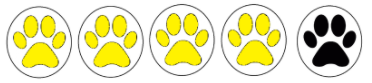
\includegraphics{exemplos/diagramas/star.PNG}
\\
Onde irá de uma “patinha” a cinco “patinhas”.
Obs: Avaliações de uma “patinhas” a duas “patinhas”, após a avaliação será apresentado um campo de texto para incluir observação de um possível problema ou feedback.

\subsection{Resposta da pergunta \ref{p12}}
\textbf{Benefício Comum:}
\begin{itemize}
    \item Apenas transportes.
\end{itemize} 
\textbf{Benefícios para o Premium:}
\begin{itemize}
    \item Aumento no ganho de pontos.
    \item Descontos adquiridos por meio do sistema de pontos, serão dobrados.
    \item Prioridade em motoristas bem avaliados.
\end{itemize}

\subsection{Resposta da pergunta \ref{p13}}
O histórico de corridas será apresentado no ícone “
    
\includegraphics[scale = 0.65]{{exemplos/diagramas/hist.PNG}}
” dentro do aplicativo, e será  composto pelas vinte últimas corridas do cliente. Podendo ter acesso às seguintes informações das corridas : Local de partida, local de destino, rota percorrida, valor da corrida, pet transportado, nome do motorista, modelo e placa do veículo, gastos adicionais (caso tiver), método de pagamento e observações da corrida.

\subsection{Resposta da pergunta \ref{p14}}
Vamos ter uma regra bastante rígida em relação aos pets que poderão ser transportados, onde aceitaremos o cadastro e transporte de somente animais domésticos. Quaisquer tentativas de transporte de animais silvestres serão repudiadas com sujeição a punições.

\subsection{Resposta da pergunta \ref{p15}}
\textbf{Caso tenha a taxa:} 
O nosso aplicativo deixará claro que animais a serviço - como cães-guia, por exemplo - estão isentos de cobrança da taxa, como estipula leis estaduais e federais.

\subsection{Resposta da pergunta \ref{p16}}
O processo de definição será por meio de grafos e informações de trânsito ao vivo, utilizando o ponto de partida e traçando a rota até o ponto de destino, podendo adicionar paradas adicionais.

\subsection{Resposta da pergunta \ref{p17}}
O aplicativo irá contar com um chat durante todas as corridas, onde o motorista e o usuário poderá trocar informações sobre possíveis consultas e detalhes do passeio com o pet, também será possível adicionar documentos (Comprovantes/Diagnósticos) ao chat.

\subsection{Resposta da pergunta \ref{p18}}
Teremos como métodos de fidelidade com o usuário o sistema de pontos, onde ao final de todas as corridas nossos usuários receberão pontos conforme a distância da corrida. O cálculo dos pontos será feito da seguinte forma (distância da viagem em metros) / 10, já para usuários premium o cálculo será ((distância da viagem em metros) / 10) + ((distância da viagem em metros) * 0.04) 
Ex (usuário comum): Viagem de 2,6 km, o usuário receberá 260 pontos.
Ex (usuário premium): Viagem de 2,6km, o usuário receberá 364 pontos.
Esses pontos poderão ser trocados em descontos para viagens futuras.

\subsection{Resposta da pergunta \ref{p19}}
Os valores dos descontos serão :\\
5\% de desconto - 600 pontos.\\
10\% de desconto - 1000 pontos.\\
30\% de desconto - 2800 pontos.\\
50\% de desconto - 4500 pontos.

% ----------------------------------------------------------
\chapter{SPRINTS}
% ----------------------------------------------------------
Essa seção contém o conteúdo desenvolvido durante todas as nossas Sprint(LINK AQUI), separados por onze períodos de uma semana cada reunião. Cara Sprint teve em média duas horas, visando respeitar a disponibilidade dos integrantes do grupo.\\

\begin{figure}
    \centering
    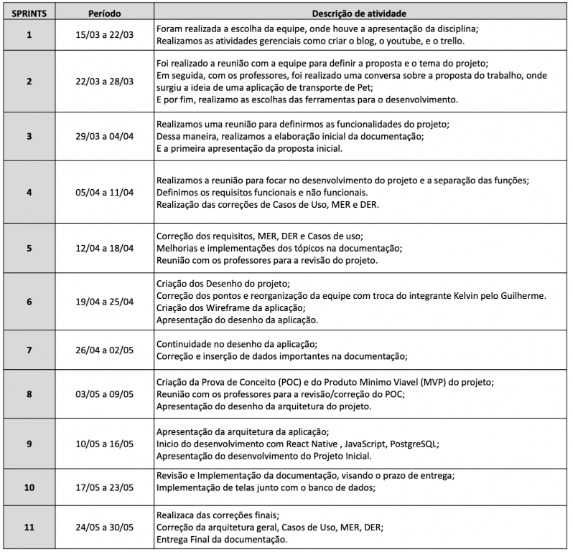
\includegraphics{exemplos/diagramas/Sprints de 11 semanas realizada pela equipe..jpeg}
    \caption{Sprints de 11 semanas realizada pela equipe.}
    \label{fig:Sprints de 11 semanas realizada pela equipe.}
    \fonte {Os Autores}
\end{figure}
% ----------------------------------------------------------
%WIREFRAME
\chapter{Wireframe}
\begin{center}
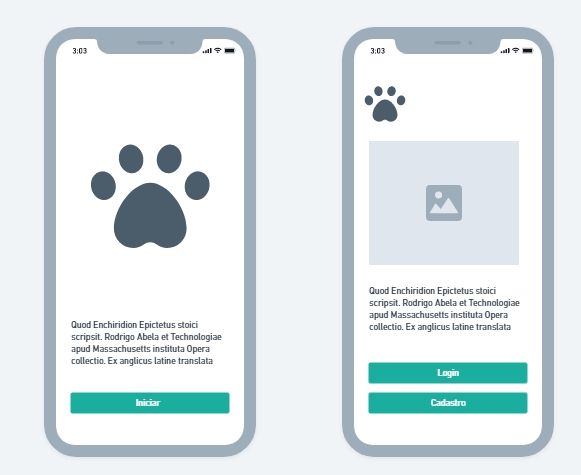
\includegraphics[width=230]{exemplos/Wireframe/Wireframe1.PNG}
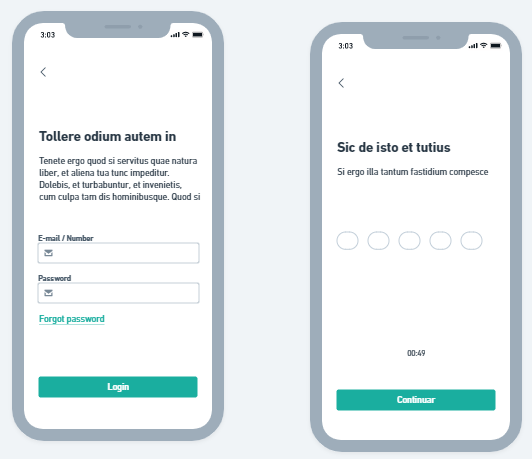
\includegraphics[width=220]{exemplos/Wireframe/Wireframe2.PNG}
\\
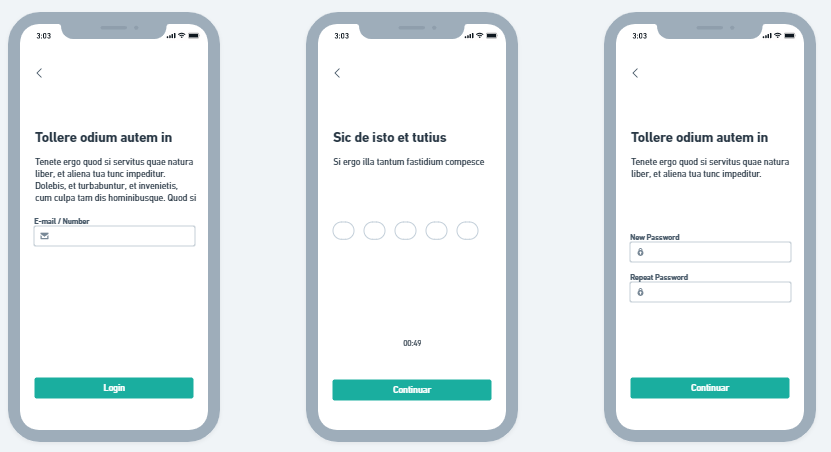
\includegraphics[width=250]{exemplos/Wireframe/Wireframe3.PNG}
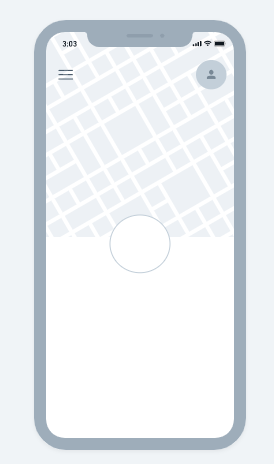
\includegraphics[width=100]{exemplos/Wireframe/Wireframe4.PNG}
\\
\includegraphics[width=250]{exemplos/Wireframe/Wireframe5.PNG}
\\
\includegraphics[width=250]{exemplos/Wireframe/Wireframe6.PNG}
\\
\includegraphics[width=250]{exemplos/Wireframe/Wireframe7.PNG}
\includegraphics[width=100]{exemplos/Wireframe/Wireframe7_1.PNG}
\\
\includegraphics[width=250]{exemplos/Wireframe/Wireframe8.PNG}
\\
\includegraphics[width=200]{exemplos/Wireframe/Wireframe9.PNG}
\includegraphics[width=200]{exemplos/Wireframe/Wireframe10.PNG}
\includegraphics[width=200]{exemplos/Wireframe/Wireframe11.PNG}
\\
\includegraphics[width=200]{exemplos/Wireframe/Wireframe12.PNG}
\includegraphics[width=80]{exemplos/Wireframe/Wireframe13.PNG}
\includegraphics[width=80]{exemplos/Wireframe/Wireframe14.PNG}
\\
\includegraphics[width=80]{exemplos/Wireframe/Wireframe15.PNG}
\end{center}

% ----------------------------------------------------------
\chapter{HISTÓRIA DE USUÁRIO }
% ----------------------------------------------------------


%REQUISITOS 
\chapter{Requisitos funcionais e não funcionais}

\section{Requisitos funcionais}
\begin{quadro}[thb]
\ABNTEXfontereduzida
\caption{Requisitos Funcionais}
\label{quadro-poluido-limpo-desalinhado}
\begin{tabular}{|l|p{2cm}|l|l|l|p{6cm}|}
\hline
\thead{RF}&\thead{Requisitos\\Funcionais} & \thead{Essencial} & \thead{Importante} & \thead{Desejável} & \thead{Descrição}\\
\hline
RF001&Permitir cadastro de usuários&\circlemark& & & O sistema tem que conceder o cadastro do usuário;\\
\hline
RF002&Permitir cadastro de usuários com conta Google&\circlemark& & & A aplicação deverá permitir que o usuário se cadastre usando a conta Google.\\
\hline
RF003&Permitir cadastro dos Pets&\circlemark& & & O sistema carece que o usuário realize o cadastro do pet (cachorro ou gato).\\
\hline
RF004&Permitir o cadastro do motorista&\circlemark& & & O app deverá aceitar o cadastro do motorista;\\
\hline
RF005&Validar e-mail&\circlemark& & & A aplicação precisa validar se o e-mail informado está correto, enviando um e-mail para o tipo usuário que está solicitando o cadastro. No máximo em 10 segundos.\\
\hline
RF006&Validar celular&\circlemark& & & A aplicação deve enviar um sms validando o número do celular do cliente cadastrado e do motorista no máximo em 10 segundos.\\
\hline
RF007&Realizar o login &\circlemark& & & O sistema deverá permitir o usuário efetuar login;\\
\hline
RF008&Escolher modalidade&\circlemark& & & Quando o cliente acessar o aplicativo o cliente escolher a modalidade comum ou premium, sendo a modalidade comum somente transporte de levar até um local específico e a premium disponibiliza serviços como: transporte e cuidado em parque, acompanhamento no veterinário e etc.\\
\hline
RF009&Quantidade de pets&\circlemark& & & A aplicação deverá solicitar que o cliente informe a quantidade de pets que irá ser transportado;\\
\hline
RF010&Escolher forma de pagamento&\circlemark& & & O cliente define a forma de pagamento como: cartão de crédito com cobrança na hora ou dinheiro depositado previamente na conta.\\
\hline
\end{tabular}
\fonte{Os autores.}
\end{quadro}

\newpage
\begin{quadro}[thb]
\ABNTEXfontereduzida
\begin{tabular}{|l|p{2cm}|l|l|l|p{6cm}|}
\hline
\thead{RF}&\thead{Requisitos\\Funcionais} & \thead{Essencial} & \thead{Importante} & \thead{Desejável} & \thead{Descrição}\\
\hline
RF011&Calcular viagem&\circlemark& & & A aplicação deverá informar ao cliente o valor da viagem antes do mesmo iniciar a viagem, levando em consideração a quantidade de pets, distância e modalidade (serviços da modalidade premium);\\
\hline
RF012&Informar tempo estimado da chegada do veículo&\circlemark& & & Através de um cálculo utilizando distância entre o passageiro e o motorista, o sistema deverá estimar um tempo de chegada. \\
\hline
RF013&Solicitar Transporte &\circlemark& & & O sistema deverá possibilitar a um usuário com perfil passageiro informar um local de origem e destino, para posteriormente fazer uma solicitação de transporte. \\
\hline
RF014&Acompanhar o pet no mapa&\circlemark& & & Tanto os passageiros como motoristas deverão poder acompanhar a posição do usuário que estiverem envolvidos na viagem.\\
\hline
RF015&Conversar com o motorista&\circlemark& & & A aplicação precisa disponibilizar  um chat para a comunicação entre o cliente e o motorista;\\
\hline
RF016&Agendar viagem& &\circlemark& & Descrição: A aplicação deverá disponibilizar a disponibilidade do motorista para o cliente, caso o mesmo deseje agendar uma nova viagem previamente.\\
\hline
RF017&Permitir confirmação da viagem&\circlemark& & & Toda viagem necessita ser confirmada tanto pelos passageiros como motoristas. \\
\hline
RF018&Finalizar viagem&\circlemark& & & A aplicação só liberará a opção de finalizar a viagem ao motorista a 1 metro do final do trajeto;\\
\hline
RF019&Permitir cancelamento da viagem&\circlemark& & & O cancelamento só será permitido caso houver um incidente pelo motorista. O sistema mostrará uma tela informando os possíveis motivos para o cancelamento.\\
\hline
RF20&Realizar avaliação da viagem&\circlemark& & & Ao término de cada viagem o passageiro irá receber uma mensagem no celular para estar avaliando a experiência da viagem e do serviço feito pelo motorista. \\
\hline
\end{tabular}
\fonte{Os autores.}
\end{quadro}
\\

%-----------------------------------------------%
\newpage
\\
\section{Requisitos não funcionais}
\begin{quadro}[thb]
\ABNTEXfontereduzida
\caption{Requisitos não funcionais}
\label{quadro-poluido-limpo-desalinhado}
\begin{tabular}{|l|p{2cm}|l|l|l|p{6cm}|}
\hline
\thead{RNF}&\thead{Requisitos\\Funcionais} & \thead{Essencial} & \thead{Importante} & \thead{Desejável} & \thead{Descrição}\\
\hline
RNF001&Interface com boa usabilidade&\circlemark& & & A aplicação deve ser intuitiva, de modo que possa ser de fácil entendimento  a todas as pessoas que acessarem o aplicativo.\\
\hline
RNF002&Resposta rápida do servidor&\circlemark& & & O software tem que fazer as consultas, histórico de viagens e a autenticação em menos de 1 segundo no lado do servidor.\\
\hline
RNF003&Verificar senha&\circlemark& & & O aplicativo necessita validar se a senha é composta por letras,caracteres especiais e número.\\
\hline
RNF004&Viagem acompanhada com o dono& &\circlemark& & O cliente deve informar via aplicativo para o motorista se irá acompanhar o seu pet. (haverá um botão no app) .\\
\hline
RNF005&Exibir senha& &\circlemark& & O aplicativo deve disponibilizar a opção de visualizar a senha.\\
\hline
RNF006&Disponibilidade do aplicativo&\circlemark& & & A aplicação deve estar disponível 99,99\% do tempo para os usuários, sete dias por semana e 24 horas por dia.\\
\hline
RNF007&Restringir a quantidade de  pets&\circlemark& & & O sistema deve informar a quantidade máxima de pets que o motorista pode transportar, tendo o máximo de 4 pets. \\
\hline
\end{tabular}
\fonte{Os autores.}
\end{quadro}


% ----------------------------------------------------------
\chapter{REGRA DE NEGÓCIOS}
% ----------------------------------------------------------


\end{apendicesenv}
% ---





% ----------------------------------------------------------
% Anexos
% Documentos gerados por outros autores
% ----------------------------------------------------------

% ---
% Inicia os anexos
% ---
\begin{anexosenv}
\anexos
% Imprime uma página indicando o início dos anexos
\partanexos

% ---
\chapter{Manual todonotes(parcial)}
\label{manual-todonotes}
% ---
\index{pdf}
% se pages = "-"  fica com arquivo completo
\includepdf[pages=1-3,scale=0.8,frame=true,pagecommand={}]{anexos/todonotes.pdf}

% ---
% Para incluir sem gerar a quebra de página inicial no anexo
\includepdf[pages=1,scale=0.7,frame=true,pagecommand=\chapter{Manual pdfpages(parcial)}\label{manual-pdfpages}]{anexos/pdfpages.pdf}
\includepdf[pages=2-3,scale=0.8,frame=true,pagecommand={}]{anexos/pdfpages.pdf}

% ---
\chapter{Manual acronym(parcial)}
\index{pdf}
% somente algumas páginas para exemplo sem borda
\includepdf[pages=1-3,frame=false,pagecommand={}]{anexos/acronym.pdf}



\includepdf[frame=true,scale=0.7,pagecommand=\chapter{Referência Rápida pifont}\label{pifont-quickref}]{anexos/pifont.pdf}


\end{anexosenv}



%---------------------------------------------------------------------
% INDICE REMISSIVO - Quando necessário 
% As palavras indexadas devem ser definidas com \index{} no texto
%---------------------------------------------------------------------
\phantompart
\printindex

%---------------------------------------------------------------------

\end{document}